\documentclass[final,openany,oneside]{hcmuitthesis}
\let\cleardoublepage\clearpage
% Config reference source file
\addbibresource{references/chapter2.bib}
\addbibresource{references/chapter3.bib}
\addbibresource{references/chapter5.bib}
\usepackage{graphicx}
\usepackage{adjustbox}
\usepackage{multirow}
\usepackage{pdfpages}
\usepackage{subcaption}
\usepackage[normalem]{ulem}

\usepackage{longtable}
\usepackage{float}

\newcolumntype{L}[1]{>{\raggedright\arraybackslash}p{#1}}

\useunder{\uline}{\ul}{}
% =========== Thay đổi thông tin tại phần này ===========
\upperuniname{ĐẠI HỌC QUỐC GIA THÀNH PHỐ HỒ CHÍ MINH}
\uniname{TRƯỜNG ĐẠI HỌC CÔNG NGHỆ THÔNG TIN}
\deptname{KHOA KHOA HỌC VÀ KỸ THUẬT THÔNG TIN}
\stumajor{CỬ NHÂN NGÀNH CÔNG NGHỆ THÔNG TIN}
\title{NGHIÊN CỨU PHƯƠNG PHÁP HỌC SÂU TRONG BÀI TOÁN DỰ ĐOÁN KẾT QUẢ HOÀN THÀNH KHÓA HỌC CỦA NGƯỜI HỌC TRÊN NỀN TẢNG MOOCS}
\titleen{RESEARCH ON DEEP LEARNING METHODS FOR PREDICTING LEARNER COURSE COMPLETION OUTCOMES ON MOOC PLATFORMS}
\supervisor{GIẢNG VIÊN HƯỚNG DẪN}
\supervisorname{ThS. NGUYỄN THỊ ANH THƯ}
\stuname{NGUYỄN VIẾT KHA \\
            NGUYỄN HOÀI PHƯƠNG}
\stunamewithid{NGUYỄN VIẾT KHA - 21520949\\
                NGUYỄN HOÀI PHƯƠNG - 21521308}
\reporttype{KHÓA LUẬN TỐT NGHIỆP}   
\instruction{GIẢNG VIÊN HƯỚNG DẪN}
\reportplace{TP. HỒ CHÍ MINH, NĂM }

% =========== Hết phần thay đổi thông tin ===========

% \newglossaryentry{ssl}{
%     name={SSL},
%     description={Secure Sockets Layer}
% }

% \newglossaryentry{api}{
%     name={API},
%     description={Application Programming Interface}
% }

\newglossaryentry{MOOCs}{
    name = {MOOCs},
    description = {Các khóa học trực tuyến mở}
}

\newglossaryentry{HINs}{
    name = {HINs},
    description = {Các mạng thông tin không đồng nhất}
}
\newglossaryentry{RNNs}{
    name = {RNNs},
    description = {Recurrent Neural Networks}
}

\makeglossaries
% Begin thesis
\setcounter{secnumdepth}{3}
\begin{document}

\coverpage%
\secondcoverpage%

% Begin above main thesis
\frontmatter
% \chapter*{\centering\Large{Thông tin hội đồng chấm khóa luận tốt nghiệp}}
\addcontentsline{toc}{chapter}{Thông tin hội đồng chấm khóa luận tốt nghiệp}
Hội đồng chấm khóa luận tốt nghiệp, thành lập theo Quyết định số 476/QĐĐHCNTT ngày 02 tháng 07 năm 2024 của Hiệu trưởng Trường Đại học Công nghệ Thông tin.
\begin{center}
    \begin{tabular}{ p{.5\textwidth} p{.3\textwidth}} 
        1. TS. Dương Việt Hằng    & Chủ tịch \\
        2. TS. Võ Nguyễn Lê Duy & Ủy viên \\ 
        3. ThS. Huỳnh Thị Thanh Thương    & Thư ký \\ 
    \end{tabular} 
\end{center}%
\chapter*{\centering\Large{Lời cảm ơn}}
\addcontentsline{toc}{chapter}{Lời cảm ơn}


% \indent Trong thời gian thực hiện khoá luận tốt nghiệp, tác giả may mắn nhận được sự giúp đỡ quý báu, hỗ trợ nhiệt tình từ rất nhiều thầy cô, anh chị, bạn vè và người thân. Trang đầu tiên này tác giả xin phép được bày tỏ những lời cảm ơn sâu sắc đến tất cả những người đã đồng hành, hỗ trợ tác giả trong khoảng thời gian vừa qua. \\

% \indent Đầu  tiên, tác giả xin gửi tri ân sâu sắc đến Trường Đại học Công nghệ Thông tin, đặc biệt là khoa Khoa học máy tính đã tạo điều kiện, môi trường học tập tươi trẻ, thoải mái, chất lượng cùng quý thầy cô luôn tạo điều kiện thuận lợi, tận tình trong quá trình học tập, nghiên cứu. Chính những kiến thức quý báu đã được truyền thụ trong suốt thời gian học tập tại trường  đã giúp tác giả nghiên cứu, thử nghiệm và hoàn thành khoá luận tôt nghiệp này. \\
% \indent Như ngọn hải đăng soi sáng con đường, thầy cô là người dẫn dắt chúng ta vượt qua những khó khăn, thử thách trong quá trình nghiên cứu. tác giả xin đặc biệt tri ân ThS. Nguyễn Thị Anh Thư, người đã tận tâm đã truyền cảm hứng, dìu dắt và hỗ trợ không chỉ về kiến thức chuyên môn mà còn về phương pháp nghiên cứu. Nhờ những kinh nghiệm quý giá mà cô truyền đạt, đã giúp tác giả hoàn thành khoá luận tốt nghiệp và sẽ luôn là hành trang quý giá theo tác giả suốt chặng đường làm việc sau này. 
% \\
% \indent Cuối cùng, tác giả xin bày tỏ lòng biết ơn chân thành đến bạn bè, gia đình và những người thân yêu, những người luôn ủng hộ, động viên và tạo động lực cho tác giả trong suốt quá trình học tập và nghiên cứu. \\
% \indent Mặc dù đã cố gắng hoàn thiện khoá luận tốt nghiệp  một cách chu đáo nhất, nhưng không thể tránh khỏi những thiếu sót và hạn chế. tác giả mong nhận được sự góp ý quý báu từ quý thầy cô và các bạn đọc để hoàn thiện hơn nữa bài luận văn của mình. \\


 Khóa luận tốt nghiệp này là một chặng đường của sự nỗ lực, tìm tòi và cũng là sự hội tụ của rất nhiều hỗ trợ quý báu. Những thành quả ngày hôm nay, chúng tôi không thể không ghi nhận và bày tỏ lòng biết ơn sâu sắc.

Trọng tâm của chặng đường này là sự đồng hành và khai mở tri thức từ cô ThS. Nguyễn Thị Anh Thư. Chúng tôi vô cùng may mắn khi được cô định hình tư duy nghiên cứu, cung cấp một la bàn định hướng rõ ràng và kiên nhẫn giải đáp mọi vướng mắc. Những kiến thức chuyên sâu cùng phương pháp tiếp cận vấn đề mà cô truyền đạt chính là chìa khóa cho đề tài này.

Bên cạnh sự dìu dắt về học thuật, chúng tôi cũng sẽ không thể đi đến đích nếu thiếu đi điểm tựa tinh thần và hỗ trợ từ quý thầy cô, nhà trường. Những lời động viên và niềm tin mà mọi người dành cho chính là sức mạnh giúp chúng tôi vượt qua những thử thách.

% Sự tận tâm và niềm say mê mà cô thể hiện trong giảng dạy đã trở thành động lực mạnh mẽ, khuyến khích chúng tôi phát triển không ngừng về mặt học thuật cũng như rèn luyện các kỹ năng thiết yếu như làm việc nhóm và tư duy phản biện. Những chia sẻ của cô đã mang đến những góc nhìn mới mẻ, thúc đẩy chúng tôi tiếp tục đào sâu nghiên cứu.

% Ngoài ra, chúng tôi xin bày tỏ lòng biết ơn chân thành tới nhà trường, quý thầy cô và bạn bè, những người đã tạo điều kiện tối ưu để chúng tôi hoàn thành khóa luận. Chúng tôi trân trọng những giá trị kiến thức và kinh nghiệm mà nhà trường đã trang bị, là yếu tố then chốt giúp chúng tôi hoàn thành tốt đề tài này.



\begin{flushright}
\textit {TP. Hồ Chí Minh, ngày 17 tháng 06 năm 2025} \\
\textit {Nguyễn Viết Kha \\
            Nguyễn Hoài Phương}
\end{flushright}


\tableofcontents
\clearpage
\listoffigures
\clearpage
\listoftables
\clearpage

\mainthesis

% Main chapter in thesis
% \chapter{Giới thiệu}
% \label{chap:chap1-introduce}

% Tại chương này, tác giả giới thiệu cấu trúc thư mục của dự án, giải thích các cài đặt, một số lưu ý trong quá trình sử dụng. Chương này cũng như báo cáo này không giới thiệu các cú pháp cơ bản như gõ phương trình, tạo bảng đơn giản, chèn hình ảnh.

% \section{Cấu trúc thư mục}

% \indent Hình \ref{fig:chap1-project-directory} mô tả cấu trúc thư mục của dự án. Thư mục \textbf{chapters} lưu các thành phần văn bản chính của dự án. Trong thư mục này chia làm ba thư mục, \textbf{\textit{back}} tương ứng với các phụ lục phía sau báo cáo.

% \begin{figure}
%     \centering
%     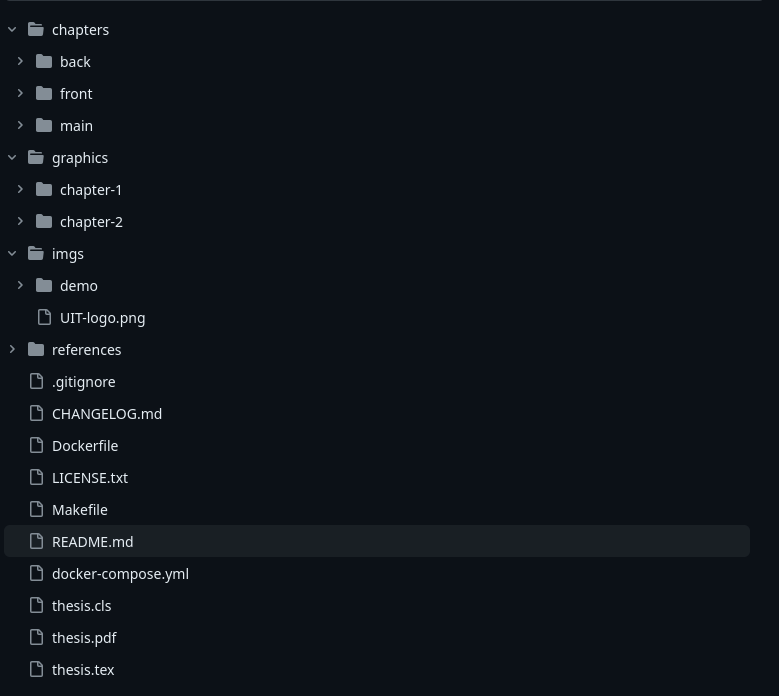
\includegraphics[scale=0.5]{chapter1/chap1-project-directory.png}
%     \caption{Cấu trúc thư mục của dự án}
%     \label{fig:chap1-project-directory}
% \end{figure}


% Thư mục \textbf{\textit{front}} tương ứng với các trang thông tin hội đồng chấm tốt nghiệp, lời cảm ơn, danh mục từ viết tắt... Thư mục \textbf{\textit{main}} chứa các chương của báo cáo. Báo cáo đánh số thứ tự riêng cho phần \textit{\textbf{front}}, trong khi phần các chương chính và phần phụ lục được đánh số giống nhau. Báo cáo đánh số trang bắt đầu từ trang tóm tắt, chữ số Ả-rập, bắt đầu bằng 1.

% Thư mục \textbf{\textit{graphics}} chứa hình ảnh được chèn vào báo cáo. Tương ứng với mỗi chương sẽ có 1 thư mục hình ảnh của chương đó.

% Thư mục \textbf{\textit{imgs}} là thư mục chứa hình ảnh của dự án, nó bao gồm các logo, watermark hoặc hình ảnh phục vụ cho document trên github. Hình chèn vào báo cáo không được lưu trong thư mục này.

% Thư mục \textbf{\textit{references}} chứa các file chỉ mục tài liệu tham khảo. Tương tự như mỗi chapter một file .tex, nó cũng có riêng một file .bib để chỉ rõ các tài liệu tham khảo nào được sử dụng trong chuong nào.

% File \textbf{\textit{thesis.cls}} là file quy định các câu lệnh, mức chỉ mục đánh số hình ảnh, bảng biểu, phần, chương. Quy định header và footer, trang  bìa.... Chi tiết xem trong file. Hãy chắc chắn rằng bạn hiểu rõ tất cả nếu muốn thay đổi gì trong file này.

% File \textbf{\textit{thesis.tex}} là file quy định cấu trúc báo cáo, chương nào trước, chương nào sau, quy định thư mục hình ảnh chèn trong báo cáo. Nó quy định thông tin người báo cáo thông qua các câu lệnh được quy định trong file .cls. 

% \section{Thay đổi các biến khi sử dụng}

% Hai bìa của luận văn được tự động tạo bởi latex. Vì vậy, có các biến được quy định để đảm nhiệm nó. Các biến cần thay đổi được đặt tại thư mục gốc, tập tin \textit{thesis.tex}, được thể hiện trong hình \ref{fig:chap1-information-variable}.

% \begin{figure}
%     \centering
%     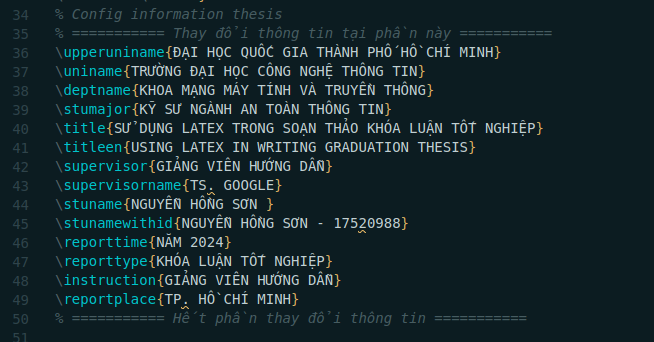
\includegraphics[scale=0.7]{chapter1/chap1-information-variable.png}
%     \caption{Phần thay đổi thông tin trang bìa}
%     \label{fig:chap1-information-variable}
% \end{figure}

% Các phần tiếp theo, quy định các nội dung được thêm vào báo cáo chính. Nếu một tập tin xuất hiện trong thư mục chapters nhưng không được khai báo bằng lệnh \textit{include} thì cũng không xuất hiện trong báo cáo. Vậy nên các chương mới bắt buộc phải được khai báo trong \textit{thesis.tex}. Các phần tài liêu tham khảo cũng được hiểu tương tự.

\chapter{Tổng quan}
\label{chap:chap1}
\section{Giới thiệu}
Công nghệ số chính là động lực cốt lõi, tạo ra một cú hích cho sự ra đời và phát triển thần tốc của các khóa học trực tuyến mở (MOOCs). Các nền tảng này đang từng bước định hình lại toàn cảnh giáo dục hiện đại thông qua tính linh hoạt, sự tiện lợi và khả năng tiếp cận không giới hạn. Làn sóng giáo dục trực tuyến này đang tạo ra một cuộc dịch chuyển trong tiêu chuẩn giáo dục toàn cầu, khẳng định vị thế của nó như một phương thức học tập ngày càng chủ đạo.

Tuy nhiên, tỷ lệ người học bỏ cuộc ở các khóa học MOOCs vẫn ở mức rất cao. Hiện tượng này không chỉ chứng tỏ các giới hạn của hệ thống mà sâu xa hơn, nó cho thấy sự thiếu kết nối hiệu quả giữa nội dung khóa học và người học. Sở dĩ có thực trạng này là do sự tác động từ hai nhóm nguyên nhân chính. Về phía nền tảng, cấu trúc học liệu đôi khi còn cồng kềnh, gây quá tải và môi trường học tập thiếu tính tương tác, hấp dẫn. Về phía người học, rào cản đến từ sự thiếu hụt kỹ năng học tập tự chủ, động lực không bền vững và thiếu một định hướng học tập rõ ràng. Trước thực trạng trên, việc đề ra các giải pháp nhằm hạ thấp tỷ lệ bỏ học là vô cùng cấp thiết.

Trong bối cảnh đó, việc phát triển các mô hình có khả năng dự đoán chính xác nguy cơ bỏ học của sinh viên được xem là một chiến lược can thiệp sớm đầy tiềm năng. Bằng việc nhận diện sớm các dấu hiệu hành vi bất thường, hệ thống có thể hỗ trợ cá nhân hóa lộ trình học, điều chỉnh phương pháp dạy, hoặc tăng cường mức độ tương tác. Mặc dù vậy, tồn tại không ít rào cản đáng kể về mặt kỹ thuật, cụ thể là:
\begin{enumerate}
    \item \textbf{Khối lượng dữ liệu khổng lồ và đa dạng của MOOCCubeX:} Dữ liệu được lấy từ các nền tảng MOOCs rất lớn, trong đó thông tin về khóa học, hồ sơ người dùng, lịch sử học tập, tương tác với nội dung và với những người học khác. Bên cạnh đó, dữ liệu có tính chất đa dạng: từ dữ liệu có cấu trúc, bán cấu trúc và không cấu trúc. Trước những đặc tính này, yêu cầu cốt lõi đặt ra là khả năng xử lý đồng thời nhiều định dạng dữ liệu khác nhau với tốc độ cao và độ chính xác tuyệt đối cùng với khối lượng dữ liệu lớn. Hệ thống cần sở hữu nền tảng mở rộng linh hoạt (scalable) để thích ứng với tốc độ sinh dữ liệu, cùng cơ chế tích hợp liền mạch cho phép đồng bộ đa nguồn thời gian thực. 

    \item \textbf{Tính không hoàn chỉnh và thiếu đồng nhất của dữ liệu:} Trong môi trường MOOC, việc người học bỏ dở khóa học giữa chừng, không hoàn thành bài kiểm tra, hoặc bỏ qua các nội dung học tập dẫn đến tình trạng dữ liệu bị phân mảnh và thiếu hụt nghiêm trọng. Thêm vào đó, nguyên nhân từ những bất cập trong quy trình thu thập và lưu trữ cũng là lý do. Sự thiếu hụt dữ liệu ảnh hưởng trực tiếp đến tính toàn vẹn và đồng nhất của bộ dữ liệu.
\end{enumerate}

Xuất phát từ những thách thức trên, nghiên cứu này đề xuất và phát triển các mô hình học sâu cho bài toán dự đoán kết quả hoàn thành khóa học của người học trên MOOCs. Cụ thể, nghiên cứu nhằm đạt được hai mục tiêu sau:
\begin{enumerate}
    \item Giải quyết thách thức dữ liệu lớn và không đầy đủ trên MOOCs: Mục tiêu này tập trung vào việc xử lý dữ liệu lớn, không đầy đủ thông qua việc tích hợp các kỹ thuật xử lý tiền kỳ như làm sạch, chuẩn hóa và đặc biệt là điền khuyết dữ liệu. Khóa luận đề xuất một giải pháp tiên tiến để suy diễn dữ liệu thiếu bằng GCN, cho phép khai thác hiệu quả cấu trúc quan hệ tiềm ẩn giữa các thực thể học tập (ví dụ: sinh viên, bài giảng, tương tác).
    
    \item Dự đoán kết quả hoàn thành khóa học trên MOOCs: Ứng dụng các mô hình học sâu nhằm khai thác hiệu quả dữ liệu học tập phong phú trong MOOCs, từ hành vi truy cập, lịch sử học tập đến mức độ tương tác với nội dung. Khóa luận này sử dụng 4 mô hình học sâu bao gồm: RNN, GRU, 4-layer stacked LSTM, BiLSTM.
\end{enumerate}
Chúng tôi mong muốn với những mục tiêu trên, khóa luận sẽ đem lại ý nghĩa trong việc nâng cao tỷ lệ duy trì học tập, giảm thiểu tình trạng bỏ học. Qua đó, giúp người học khai thác tối đa tiềm năng của các nền tảng MOOCs và mở rộng cơ hội tiếp cận tri thức.


% Trong bối cảnh hiện đại, giáo dục đã có cách mạng lớn đó là hệ thống giáo dục trực tuyến hiện đại. Hệ thống giáo dục hiện đại chứng kiến sự ra đời và phát triển mạnh mẽ của các nền tảng học trực tuyến mở (MOOC), mở ra vô vàn cơ hội tiếp cận tri thức cho mọi đối tượng đến từ mọi nơi trên thế giới thông qua giảng dạy trực tuyến. Để thực hiện trên quy mô lớn này, các hệ thống giáo dục này luôn có kho tàng khổng lồ các khoá học phong phú, đa dạng để đáp ứng cho nhiều đối tượng người học. Do đó, người học thường xuyên gặp khó khăn trong việc xác định, chọn lựa môn học phù hợp với mong muốn và năng lực của bản thân. Để giải quyết thực trạng này, việc nghiên cứu và xây dựng một hệ thống khuyến nghị môn học hiệu quả cho các nền tảng MOOC là hết sức cần thiết để giải quyết các thực trạng sau:

% Trong bối cảnh giáo dục hiện đại, hệ thống khuyến nghị đã chứng minh được giá trị của mình bằng cách cung cấp các gợi ý phù hợp cho các cơ sở giáo dục, giáo viên và học sinh. Đặc biệt, với sự bùng nổ của các nền tảng MOOC, việc xây dựng một hệ thống khuyến nghị môn học hiệu quả trở thành một nhu cầu cấp thiết.

% Nhằm giải quyết các thách thức lớn nêu trên và khai thác hiệu quả dữ liệu Big Data từ các nền tảng MOOC, tác giả đề xuất đề tài "Nghiên cứu phương pháp cải tiến hệ thống khuyến nghị môn học dựa trên dữ liệu lớn từ các nền tảng MOOC" với hai mục tiêu chính:
% \begin{enumerate}
%     \item Tập trung giải quyết các thách thức từ dữ liệu lớn từ MOOC. Xử lý và khai thác dữ liệu hiệu quả, mô hình hoá các tương tác của người dùng để thu được dữ liệu có ích để nắm bắt được sở thích, tính cá nhân hoá của người dùng.
%     \item Xây dựng hệ thống khuyến nghị hiện đại, tận dụng dữ liệu lớn từ MOOC để đề xuất môn học phù hợp với từng người dùng.
% \end{enumerate}

\section{Bài toán nghiên cứu}
Với những ưu điểm về tính linh hoạt, tiện lợi và khả năng tiếp cận trên quy mô lớn, các nền tảng MOOCs đã khẳng định vị thế mạnh mẽ. Vượt ra ngoài chức năng là một không gian học tập độc lập, MOOCs hiện nay còn được tích hợp sâu rộng vào giáo dục bậc đại học, hình thành nên các mô hình học tập kết hợp (Blended Learning - BL) năng động, đáp ứng hiệu quả nhu cầu đa dạng của người học trong thời đại số \cite{de2021use}.

Hew và cộng sự (2014) \cite{hew2014students} đã chỉ ra ba nhóm động lực chính của người học. Thứ nhất là nhu cầu trau dồi tri thức, bao gồm việc khám phá các lĩnh vực mới hoặc đào sâu chuyên môn. Thứ hai là mong muốn chinh phục các thử thách cá nhân và kiểm chứng năng lực bản thân. Thứ ba là mục tiêu thu thập các chứng chỉ nhằm phục vụ cho việc học tập lên cao hoặc phát triển sự nghiệp. Sự đa dạng trong các động cơ này cho thấy tiềm năng to lớn của MOOCs trong việc đáp ứng một phổ rộng các mục tiêu giáo dục cá nhân.

Một đặc điểm ưu việt khác của MOOCs so với giáo dục truyền thống là khả năng thu thập và phân tích dữ liệu học tập ở quy mô lớn. Ví dụ thời lượng tương tác với video bài giảng, tiến độ hoàn thành bài tập, mức độ tham gia diễn đàn và kết quả cuối kỳ đều được ghi nhận. Nguồn dữ liệu lớn (big data) này mở ra cơ hội để nhận diện các xu hướng học tập, giúp phát hiện sớm các dấu hiệu có nguy cơ bỏ học, từ đó có các biện pháp can thiệp kịp thời.

Một trong những rào cản lớn khiến người học chùn bước là khó khăn khi tương tác trong một ngôn ngữ khác biệt, đặc biệt đối với những người học đến từ các nước không sử dụng tiếng Anh. Khi tương tác với người học khác trong môi trường trực tuyến toàn cầu, những rào cản này có thể làm tăng sự khó khăn trong giao tiếp, trao đổi ý tưởng và tiếp thu kiến thức \cite{ma2023leveraging}.

Thực tế cho thấy, chỉ khoảng 10\% số người đăng ký hoặc thậm chí ít hơn hoàn thành các khóa học phổ biến \cite{hew2014students}. Nhiều nguyên nhân đã được chỉ ra, bao gồm: thiếu động lực học tập bền vững, thiếu kiến thức nền tảng cần thiết để theo kịp nội dung, sự không tập trung vào diễn đàn tương tác, khó hiểu bài giảng khi thiếu hỗ trợ kịp thời, yêu cầu khóa học mơ hồ, và đặc biệt là không đủ thời gian do các ưu tiên khác trong cuộc sống, dẫn đến tình trạng trì hoãn và cuối cùng là bỏ cuộc.

Chính vì đó, trong thời gian qua, các nhà nghiên cứu xem xét một cách toàn diện nhiều yếu tố, từ đặc điểm cụ thể của từng khóa học, trường đại học, nền tảng công nghệ cung cấp MOOC, cho đến hồ sơ và đặc điểm cá nhân của người học. Mục tiêu cuối cùng là tìm ra những yếu tố chính dẫn đến quyết định hoàn thành hay bỏ dở khóa học của người học. Việc xác định sớm kết quả hoàn thành khóa học và có cơ chế can thiệp kịp thời để giảm thiểu nguy cơ tiềm ẩn đã được chứng minh là những giải pháp then chốt giúp giải quyết thách thức này.\cite{baneres2023early, andres2018studying}.
\begin{figure}[H]
    \centering
    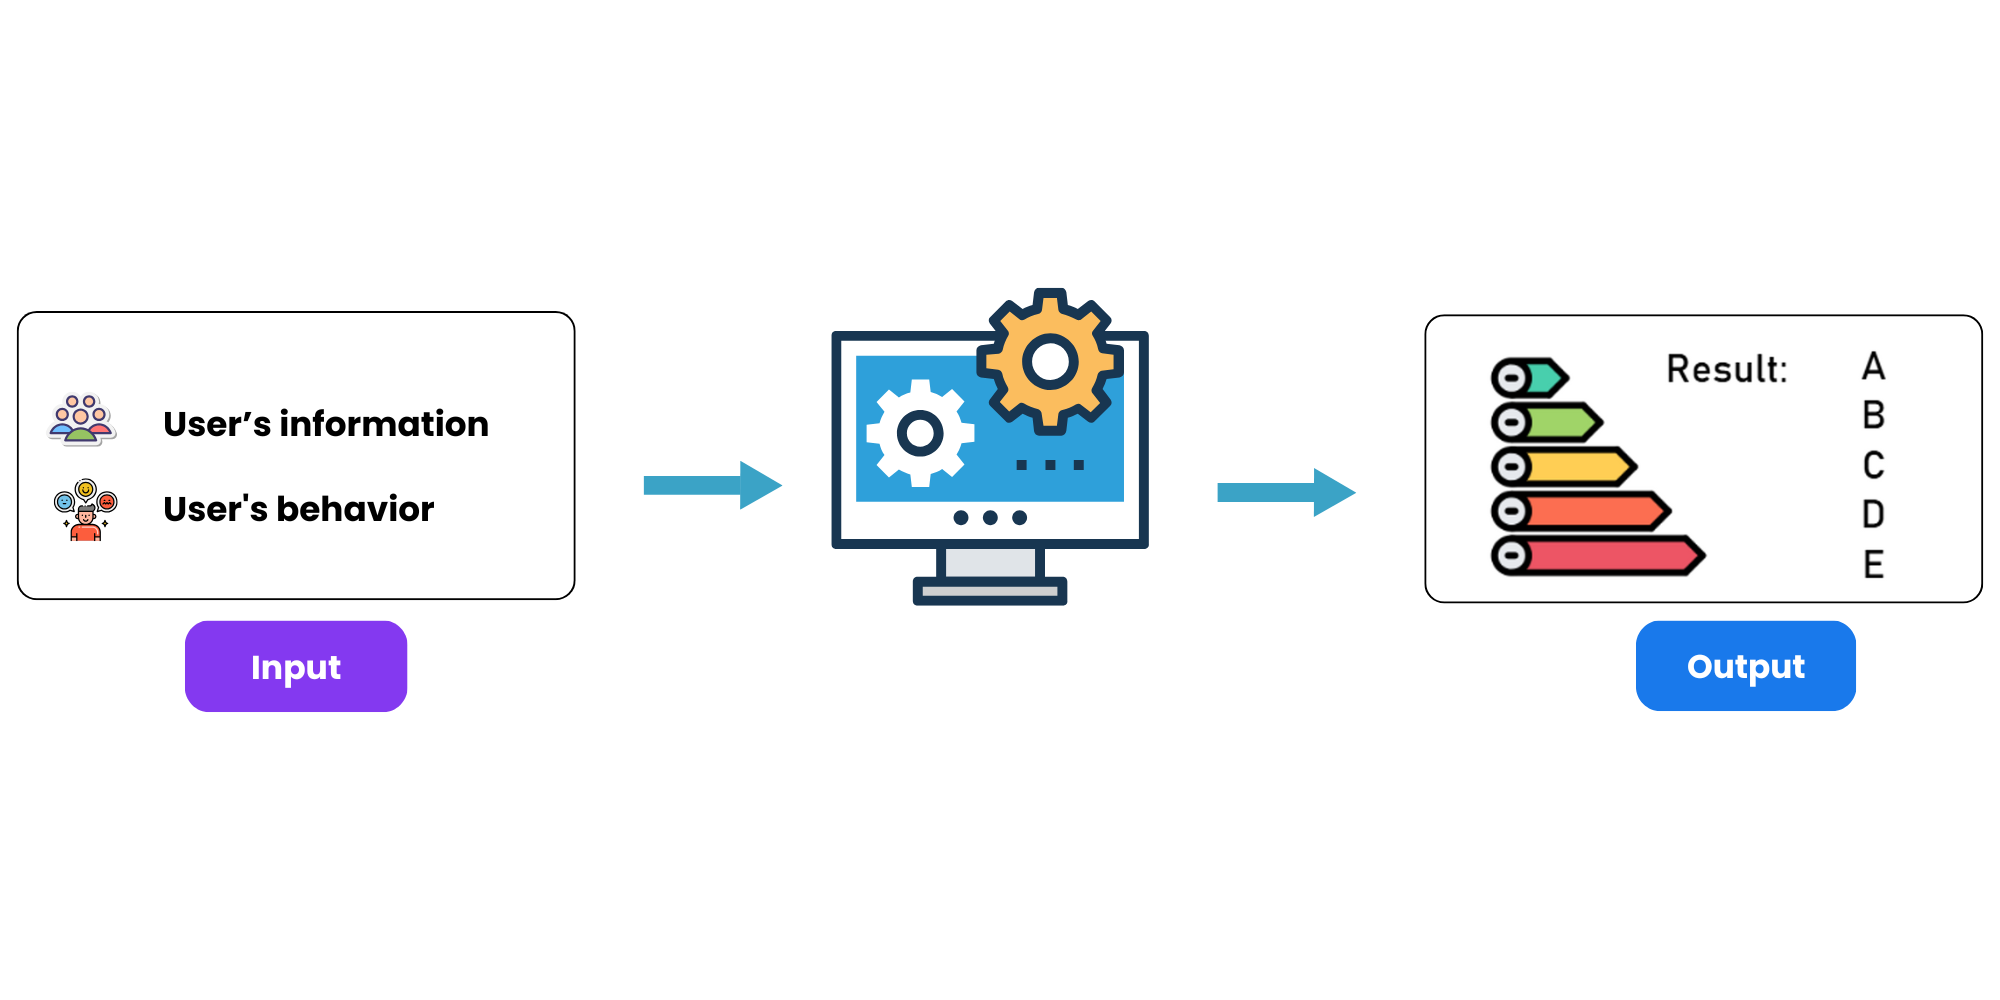
\includegraphics[width = 0.8\textwidth]{imgs/input-output.png}
    \caption{Minh hoạ input và output của bài toán.}
    \label{fig:input_output}
\end{figure}

Bài toán mà chúng tôi đặt ra là dự đoán kết quả hoàn thành khóa học và đưa ra cảnh báo sớm trên các nền tảng MOOCs dựa trên dữ liệu học tập của học viên. Cụ thể như sau:

\begin{itemize}
    \item \textbf{Input:} Dữ liệu học tập của học viên, bao gồm hành vi học tập (thời gian học, số bài tập đã hoàn thành, điểm số), đặc điểm cá nhân, thông tin khóa học, thời gian hoàn thành bài tập và hành vi tương tác (số lần bình luận, phản hồi trên diễn đàn).

    \item \textbf{Output:} Dự đoán kết quả hoàn thành khóa học của người học phân loại theo 5 cấp độ (A: Xuất sắc, B: Giỏi, C: Đạt yêu cầu, D: Không đạt, E: Chưa hoàn thành).
\end{itemize}
Nguồn dữ liệu từ nền tảng MOOC thường có tỷ lệ dữ liệu bị khuyết rất cao, thậm chí lên đến hơn 60\%. Tình trạng này gây trở ngại trong việc xử lý và nắm bắt hành vi người học, song song đó còn làm giảm đáng kể hiệu suất mô hình học sâu, vốn rất nhạy cảm với sự thiếu hụt dữ liệu.

Để giải quyết thách thức về dữ liệu thiếu, khóa luận này triển khai Mạng đồ thị tích chập (GCN) như một phương pháp cốt lõi để suy diễn và bổ sung các giá trị khuyết. Cách tiếp cận này vượt trội hơn so với các kỹ thuật truyền thống vốn xử lý từng điểm dữ liệu một cách độc lập. Thay vào đó, GCN cho phép khai thác cấu trúc quan hệ phức tạp giữa các thực thể như sinh viên, hoạt động học tập và đặc điểm khóa học, từ đó đưa ra các dự đoán về giá trị thiếu một cách thông minh và chuẩn xác hơn. Việc áp dụng GCN mang lại lợi ích kép: vừa nâng cao chất lượng dữ liệu đầu vào, vừa tạo tiền đề thuận lợi để cải thiện hiệu suất dự báo của các mô hình học sâu. Khi dữ liệu được xử lý một cách toàn diện, các pipeline học sâu có thể "học" được hành vi người dùng hiệu quả hơn, dẫn đến khả năng dự báo chính xác về kết quả học tập, mức độ gắn kết và nguy cơ bỏ học.

% Cấu trúc của các phần còn lại trong khóa luận được tổ chức như sau. Đầu tiên, chúng tôi sẽ đi sâu vào việc phân tích nền tảng lý thuyết và các công trình liên quan đến bài toán dự đoán kết quả học tập. Tiếp theo, một chương riêng sẽ trình bày chi tiết quá trình thực nghiệm và kết quả đánh giá, nhằm chứng minh hiệu quả vượt trội của phương pháp GCN trong bối cảnh dữ liệu MOOCs. Cuối cùng, phần kết luận sẽ tóm lược những đóng góp chính của nghiên cứu và đề xuất các hướng phát triển trong tương lai.

\section{Mục tiêu}

 Phương pháp GCN-I được kỳ vọng sẽ cải thiện chất lượng dữ liệu đầu vào, từ đó cải thiện đáng kể độ chính xác của mô hình. Bằng cách xử lý hiệu quả các giá trị thiếu hụt, mô hình có thể tận dụng tối đa thông tin sẵn có, giúp dự đoán trở nên tin cậy và chính xác hơn.

Các mục tiêu cụ thể của khóa luận được triển khai qua bốn giai đoạn chính như sau:
\begin{enumerate}
    \item \textbf{Khảo sát các phương pháp hiện tại}: Giai đoạn đầu sẽ thực hiện một tổng quan lý thuyết sâu rộng về các công trình hiện có. Trọng tâm là phân tích các pipeline học sâu và các phương pháp điền khuyết dữ liệu đã được áp dụng trên nền tảng MOOCs. Quá trình này giúp hiểu rõ đặc điểm cấu trúc, nguyên lý hoạt động, điểm mạnh và thiếu sót của mô hình. Việc phân tích sâu sắc các phương pháp hiện tại không chỉ làm rõ các phương pháp hiện có và là nền tảng cho nghiên cứu, mà còn giúp xác định khoảng trống nghiên cứu và tiếp cận bài toán theo cách đúng đắn và phù hợp.
    \item \textbf{Khai phá và phân tích đặc trưng dữ liệu MOOCs}: Giai đoạn này khai thác và phân tích chuyên sâu bộ dữ liệu quy mô lớn từ nền tảng MOOCs. Quy trình bao gồm các bước thu thập, tiền xử lý và phân tích, nhằm trích xuất những thông tin cốt lõi liên quan đến hành vi người học. Mục tiêu là nhận diện các đặc trưng nổi bật và các xu hướng học tập tiềm ẩn, từ đó đề xuất các phương pháp xử lý và phân tích dữ liệu hiệu quả, có định hướng rõ ràng.

    \item \textbf{Đề xuất và triển khai phương pháp cải thiện dữ liệu}: Dựa trên các đặc điểm dữ liệu và tổng hợp từ các công trình đi trước, khóa luận đề xuất GCN-I, một phương pháp điền khuyết dữ liệu dựa trên đồ thị. Phương pháp này tận dụng khả năng lan truyền thông tin giữa các nút lân cận trong cấu trúc đồ thị để suy luận và điền vào các giá trị bị thiếu một cách chuẩn xác.

    \item \textbf{Thiết kế kịch bản thực nghiệm và đánh giá hiệu năng}: Giai đoạn cuối cùng của khóa luận tập trung vào việc xây dựng và thực thi các kịch bản thực nghiệm để kiểm chứng và định lượng hiệu quả của phương pháp đã đề xuất. Quá trình đánh giá sẽ được tiến hành trên cả hai khía cạnh: chất lượng dữ liệu sau khi xử lý và hiệu suất của mô hình dự đoán. Các kết quả thu được không chỉ nhằm định lượng mức độ cải thiện về độ chính xác và khả năng khái quát hóa, mà còn góp phần khẳng định giá trị và tiềm năng ứng dụng thực tiễn của GCN-I trong bối cảnh dữ liệu lớn và thưa thớt.
\end{enumerate}
\section{Phạm vi và đối tượng nghiên cứu}
% \subsection{Bộ dữ liệu MOOCCubeX}
Đề tài nghiên cứu tập trung vào việc cải thiện chất lượng dữ liệu nhằm nâng cao kết quả dự đoán của các mô hình học sâu trong bài toán dự đoán kết quả hoàn thành khóa học của người học trên nền tảng MOOCs. Nghiên cứu tích hợp hệ thống nhãn đánh giá toàn diện và ứng dụng các thư viện, công cụ hàng đầu như scikit-learn, TensorFlow, Keras và PyTorch. Chúng tôi sử dụng bộ dữ liệu được cung cấp từ XueTangX - nền tảng học tập trực tuyến của Trung Quốc trong giai đoạn 2019-2020.

Đối tượng nghiên cứu là người học tham gia học tập trên nền tảng MOOCs, dữ liệu thu thập bao gồm thông tin nhân khẩu học vả hành vi học tập. Tập dữ liệu tổng hợp quy mô lớn với 4.216 khóa học, 230.263 video giảng dạy, 358.265 bài tập, 637.572 khái niệm học tập chi tiết cùng hơn 296 triệu bản ghi hành vi thô từ 3.330.294 người học.

\section{Cấu trúc báo cáo khóa luận}
Cấu trúc của khóa luận bao gồm 7 chương chính, được trình bày như sau:

\begin{itemize}
\item \textbf{Chương \ref{chap:chap1} - Tổng quan:} Trình bày bối cảnh, mục tiêu, phạm vi, đối tượng nghiên cứu và cấu trúc khóa luận.
\item \textbf{Chương \ref{chap:chap2} - Các công trình nghiên cứu liên quan:} Tổng hợp các công trình tiêu biểu về mạng nơ-ron đồ thị và học sâu.
 \item \textbf{Chương \ref{chap:chap3} - Cơ sở lý thuyết:} Cung cấp kiến thức nền về học sâu, GCN và các phương pháp làm giàu dữ liệu.
\item \textbf{Chương \ref{chap:chap4} - GCN-I: Phương pháp suy diễn giá trị khuyết:} Giới thiệu, bộ dữ liệu thực nghiệm và trình bày phương pháp đề xuất.
\item \textbf{Chương \ref{chap:chap5} - Thực nghiệm và đánh giá:} Mô tả quá trình thực nghiệm, chỉ số đánh giá và kết quả thực nghiệm.
\item \textbf{Chương \ref{chap:chap6} - SmartEduTrack:} Giới thiệu hệ thống hỗ trợ theo dõi học tập thông minh nhằm phục vụ quản lý giáo dục.
\item \textbf{Chương \ref{chap:chap7} - Kết luận và hướng phát triển:} Tổng kết những đóng góp chính và đề xuất các hướng nghiên cứu trong tương lai.
 \item \textbf{Tài liệu tham khảo:} Danh mục các công trình đã được trích dẫn trong khóa luận.
\end{itemize}
 
 % Nghiên cứu này sẽ sử dụng dữ liệu từ các nền tảng MOOCs thực tế như Coursera\footnote{https://www.coursera.org/}, edX\footnote{https://www.edx.org/}, XuetangX\footnote{https://www.xuetangx.com/},... để đảm bảo tính thực tiễn khi đánh giá.
% \subsection{Các kiến trúc dữ liệu lớn}
% Khoá luận tập khảo sát và ứng dụng các kiến trúc dữ liệu lớn hiện đại. Các kiến trúc này được xây dựng trên nền tảng của nhiều công nghệ và thành phần khác nhau, kết hợp chặt chẽ để giải quyết các thách thức đặc thù của dữ liệu lớn. Việc thiết kế kiến trúc dữ liệu lớn đòi hỏi sự cân nhắc kỹ lưỡng về hiệu năng, khả năng mở rộng, tính linh hoạt và bảo mật. Các thành phần phổ biến của một kiến trúc dữ liệu lớn bao gồm nguồn dữ liệu, hệ thống lưu trữ, xử lý dữ liệu theo lô và theo luồng, kho dữ liệu phân tích, phân tích và báo cáo, và điều phối. 
 
%  Một số kiến trúc dữ liệu lớn phổ biến hiện nay có thể kể đến như Data Warehouse, Data Lake và Data Lakehouse.
    
% \subsection{Mô hình khuyến nghị}
% nghiên cứu sẽ tập trung vào phát triển và cải tiến các mô hình khuyến nghị môn học. Đây là những thuật toán học máy hoặc học sâu phức tạp, có khả năng dự đoán sở thích và mức độ phù hợp của người dùng với các khóa học khác nhau, dựa trên dữ liệu về người dùng, khóa học và tương tác của họ. Các mô hình này thường được phân loại theo phương pháp tiếp cận, bao gồm lọc cộng tác, lọc dựa trên nội dung và các phương pháp kết hợp. 

% Nghiên cứu này tập trung vào các mô hình khuyến nghị tuần tự như SASRec\cite{sasrec} và BERT4Rec\cite{bert} đồng thời cũng đánh giá với các mô hình cổ điển như BPR\cite{bpr} và NCF\cite{ncf}.

\chapter{Công trình nghiên cứu liên quan}
\label{chap:chap2}
\section{Graph neural networks}

\begin{figure}
    \centering
    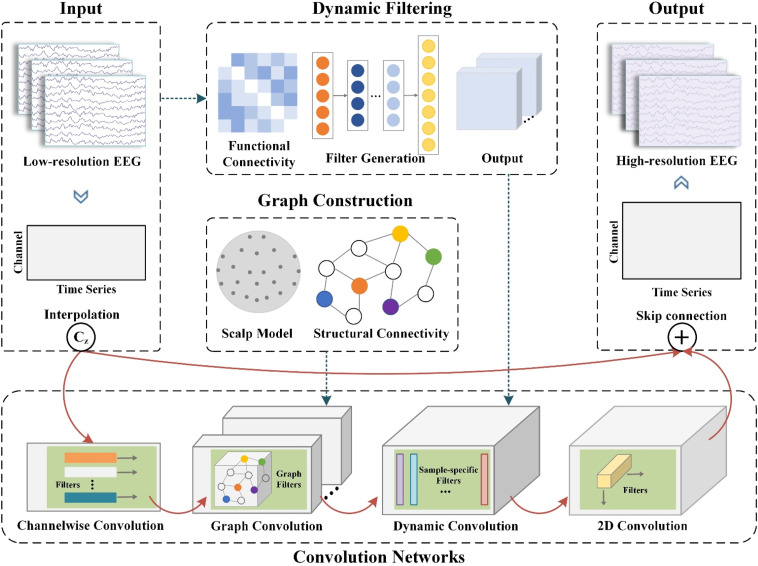
\includegraphics[width = 0.8\textwidth]{imgs/graph-convolutional-networks.jpg}
    \caption{Minh hoạ cấu trúc graph convolutional networks}
    \label{fig:CF_CBF}
\end{figure}
Mạng đồ thị (Graph Networks) là một khái niệm trong lĩnh vực trí tuệ nhân tạo và học máy. Các thực thể riêng lẻ trong mạng đồ thị không chỉ được xem xét độc lập, mà mối quan hệ giữa chúng còn được coi trọng không kém bản thân các thực thể đó. Theo Battaglia và cộng sự (2018) \cite{battaglia2018relational}, các thực thể chính là các nút (nodes), và những mối liên kết tương tác giữa chúng là các cạnh (edges). Cấu trúc này cho phép chúng ta nắm bắt được sự phụ thuộc lẫn nhau và các tương tác phức tạp, điều mà các mô hình truyền thống thường bỏ qua.

Một hiện thực tiêu biểu và đang phát triển mạnh mẽ của cách tiếp cận này là Mạng Nơ-ron Đồ thị (Graph Neural Networks - GNNs). GNNs thực chất được sử dụng chủ yếu cho dữ liệu có cấu trúc dạng đồ thị. Sức mạnh cốt lõi của GNNs nằm ở khả năng truyền tải và kết hợp thông tin giữa các nút nhờ vào các mối liên kết trên đồ thị. Quá trình này giúp GNNs học được những biểu diễn dữ liệu vô cùng phong phú và có ý nghĩa cấu trúc tổng thể của toàn bộ đồ thị. Nhờ vậy, GNNs được sử dụng để phân tích các mối quan hệ trong mạng xã hội, dự đoán hành vi người dùng hoặc xây dựng các hệ thống khuyến nghị cá nhân hóa \cite{wu2022graph, gao2022hetinf, min2021stgsn}.

Bên cạnh các ứng dụng đã được khẳng định trong phân tích mạng xã hội và hệ thống khuyến nghị, một hướng ứng dụng khác của GNNs, đặc biệt là trong bối cảnh dữ liệu thực tế, là bù đắp (imputation) các giá trị khuyết trong dữ liệu đồ thị. GNNs có thể khai thác toàn bộ cấu trúc đồ thị, đây là một điểm nổi bật và vượt trội. Thay vì chỉ xử lý từng điểm dữ liệu một cách độc lập hoặc cục bộ, GNNs tích hợp thông tin từ cấu trúc tổng thể của đồ thị. Điều này cho phép GNNs suy diễn và điền các giá trị thiếu với độ chính xác cao hơn hẳn, bởi vì chúng không chỉ dựa vào dữ liệu có sẵn mà còn tính đến các mối quan hệ giữa các thực thể. Nhờ vậy, GNNs có khả năng tích hợp thông tin, đồng thời học được các biểu diễn tiềm ẩn phản ánh sâu sắc cấu trúc nội tại của dữ liệu.

Tiềm năng của các phương pháp dựa trên GNNs đã được chứng thực qua nhiều nghiên cứu thực tiễn. Một minh chứng tiêu biểu là công trình của Spinelli và cộng sự (2020) \cite{spinelli2020missing}, trong đó các tác giả đã cho thấy hiệu quả của việc áp dụng GCNs – một biến thể phổ biến của GNNs – để xử lý dữ liệu thiếu trong các lĩnh vực phức tạp như ô nhiễm môi trường, y tế và khoa học vật lý. Những kết quả tích cực này tạo ra một cơ sở khoa học vững chắc, gợi mở tiềm năng ứng dụng GCNs vào lĩnh vực giáo dục, đặc biệt là để cải thiện chất lượng dữ liệu cho các khóa học trực tuyến mở (MOOCs).

Tóm lại, năng lực vượt trội của GNNs trong phân tích mạng xã hội và các lĩnh vực khác đã được làm rõ. Năng lực này càng trở nên nổi bật khi GNNs thể hiện lợi thế vượt trội, đặc biệt đối với bộ dữ liệu thưa thớt. Khả năng đặc biệt này đã giúp cho GNNs trở nên phù hợp với bài toán của các khóa học trực tuyến mở (MOOCs). Trong môi trường MOOC, việc thu thập dữ liệu hành vi người học thường gặp phải nhiều gián đoạn, dẫn đến dữ liệu không đầy đủ. GNNs mang đến một giải pháp tiềm năng để biến những bộ dữ liệu tưởng chừng "khuyết tật" này thành nguồn tài nguyên giá trị, từ đó giúp các mô hình học sâu đưa ra những phân tích và dự đoán chính xác hơn.


% % Trong nghiên cứu này, các mô hình khuyến nghị được đề cập đều được xây dựng dựa trên kiến trúc Transformer, một mạng nơ-ron sâu đã tạo nên bước đột phá trong lĩnh vực xử lý ngôn ngữ tự nhiên (NLP) \cite{transformer}. Kể từ ngày được công bố, Transformer đã dần trở thành một chuẩn mực trong nhiều lĩnh vực khác nhau, trong đó có các hệ thống khuyến nghị. Nhờ vào khả năng vượt trội trong việc nắm bắt các mối quan hệ phức tạp trong dữ liệu với cốt lõi là cơ chế attention, đặc biệt là self-attention, cho phép Transformer xử lý thông tin một cách song song và hiệu quả, không bị giới hạn bởi các ràng buộc tuần tự như trong các mô hình \gls{RNNs} truyền thống. Điều này giúp Transformer có thể hiểu rõ hơn về ngữ cảnh và ý nghĩa của dữ liệu, từ đó đưa ra các dự đoán và gợi ý chính xác hơn. 
% % % \begin{figure}[t]
% % %     \centering
% % %     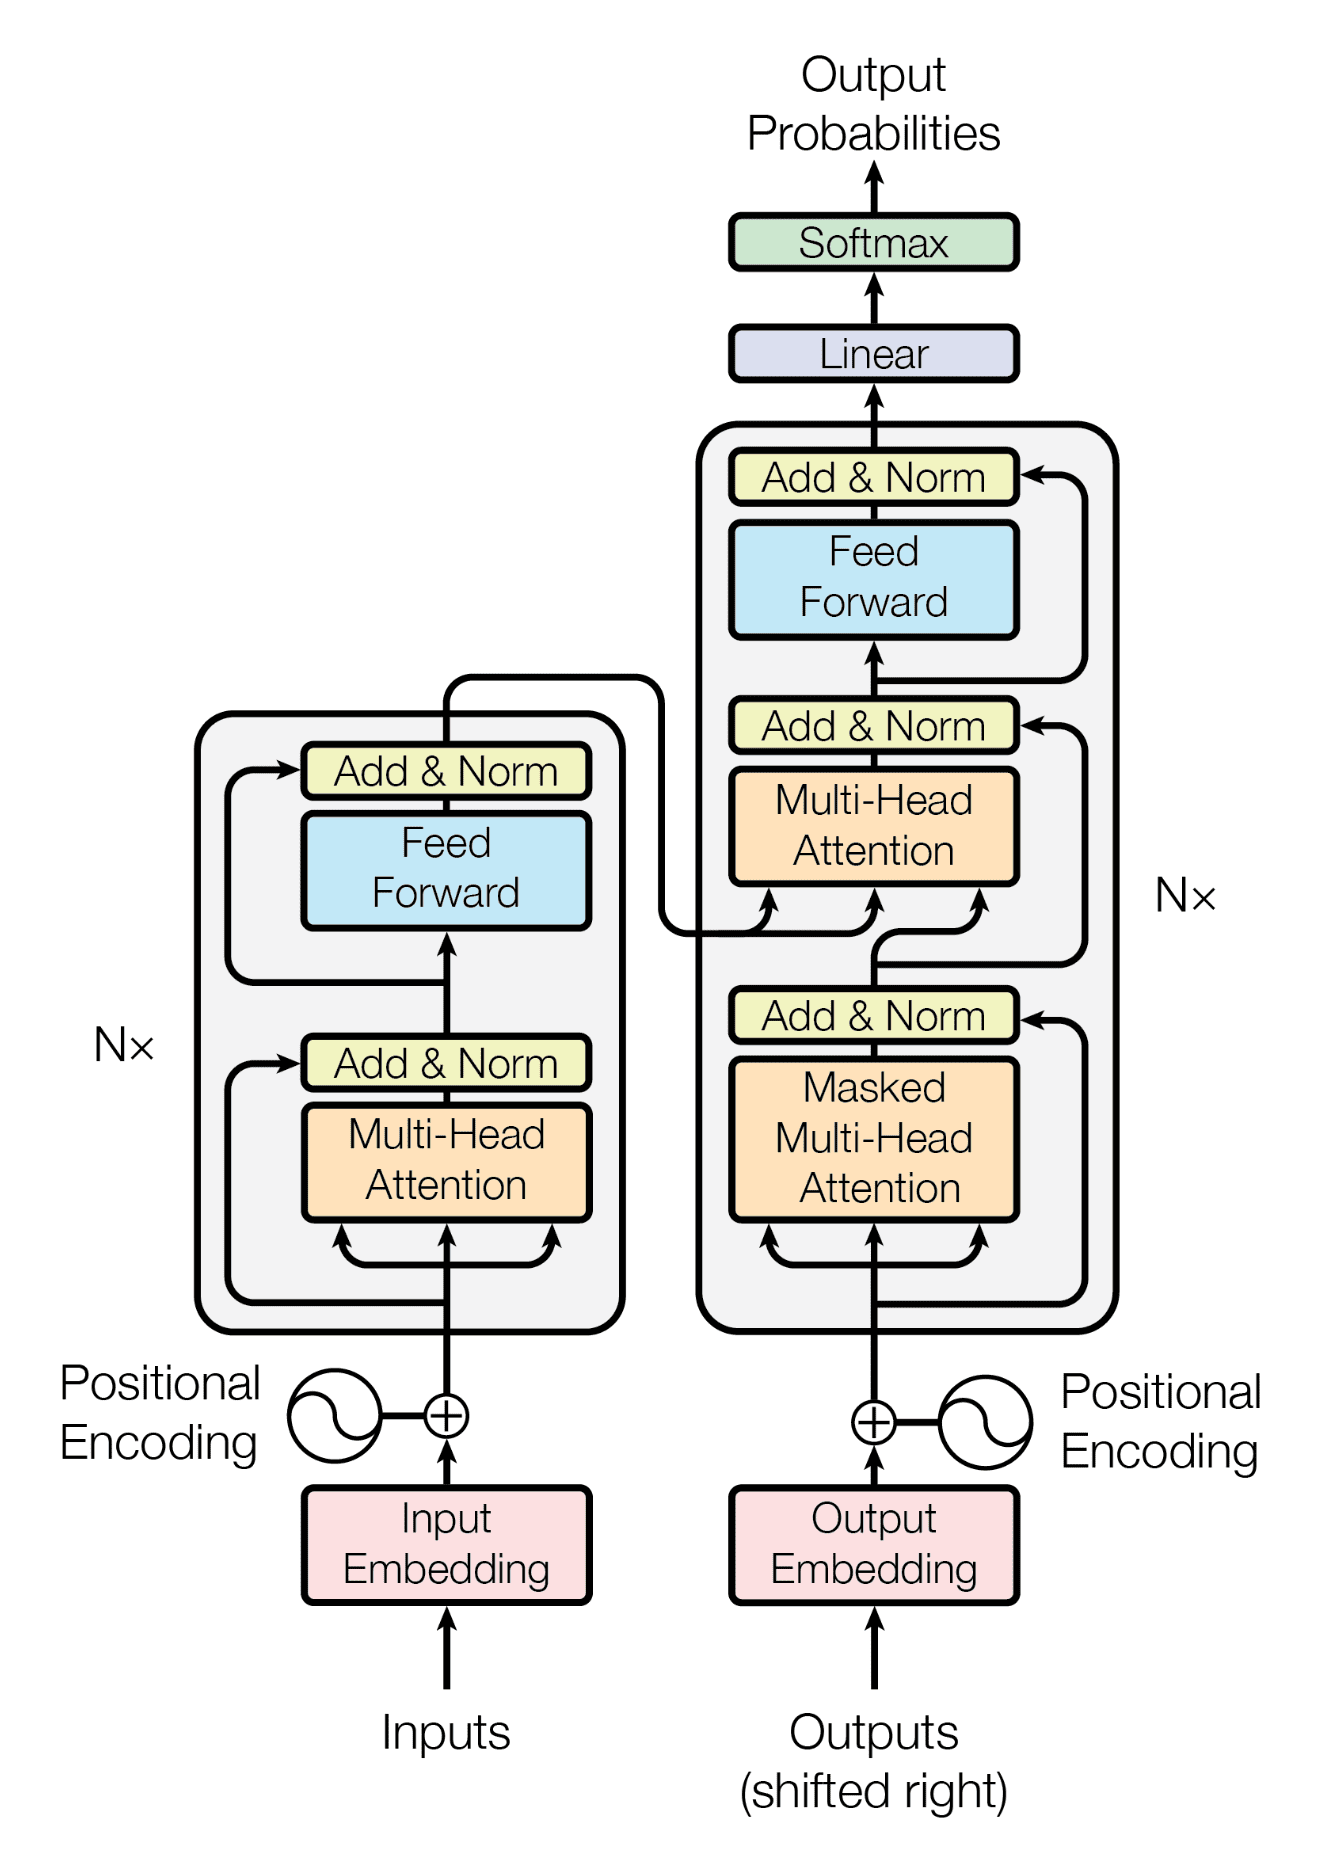
\includegraphics[width = 0.5\textwidth]{imgs/attention_research_1.png}
% % %     \caption{Kiến trúc Transformer}
% % %     \label{fig:transformer}
% % % \end{figure}
% % Như hình \ref{fig:transformer}, Transformer gồm hai thành phần chính: Encoder và Decoder. Tuy nhiên, trong nhiều ứng dụng như hệ thống khuyến nghị, chỉ thành phần Encoder được sử dụng.
% % \subsubsection{Encoder}
% % Encoder của Transformer bao gồm một số lớp lặp lại, mỗi lớp bao gồm hai thành phần chính:
% % \begin{itemize}
% %     \item \textbf{Cơ chế Multi-Head và Self-Attention:} Là cốt lõi của Transformer. Cơ chế này cho phép mỗi phần tử trong chuỗi đầu vào tự đánh giá mức độ quan trọng của mình so với các phần tử khác, từ đó xác định mối liên hệ và ảnh hưởng lẫn nhau. Nhờ vậy, Transformer có khả năng nắm bắt đồng thời nhiều loại quan hệ khác nhau, từ gần đến xa, giúp mô hình hiểu rõ hơn về cấu trúc và ngữ nghĩa của dữ liệu.
% %     \item \textbf{Feed-Forward Neural Network:} Sau khi áp dụng self-attention, kết quả đầu ra được đưa đến một mạng nơ-ron chuyển tiếp. Mạng này gồm hai lớp nơ-ron với hàm kích hoạt phi tuyến, đóng vai trò như một bộ lọc giúp học được các đặc trưng phức tạp và trừu tượng từ dữ liệu.
% % \end{itemize}
% % Mỗi lớp trong Encoder cũng có các cơ chế chuẩn hóa và cơ chế dropout để cải thiện tính ổn định và giảm thiểu hiện tượng overfitting.

% % \subsubsection{Decoder}
% % Mặc dù không thường xuyên suất hiện trong các hệ thống khuyến nghị, nhưng thành phần Decoder của Transformer cũng bao gồm các lớp multi-head attention và feed-forward tương tự như trong Encoder. Điểm khác biệt chính nằm ở cơ chế attention đặc biệt của Decoder, cho phép nó tương tác với đầu ra của Encoder. Nhờ đó, Decoder có thể tổng hợp thông tin từ cả dữ liệu đầu vào và ngữ cảnh hiện tại, từ đó đưa ra những dự đoán chính xác và phù hợp hơn.

% % \subsubsection{Self-Attention và Multi-Head Attention}
% % Cơ chế self-attention là một trong những yếu tố cốt lõi làm nên sức mạnh của Transformer. Nó cho phép mô hình tự động tập trung vào những phần quan trọng của dữ liệu đầu vào bằng cách tính toán một bộ trọng số thể hiện mức độ liên quan giữa các phần tử trong chuỗi. Công thức cho self-attention bao gồm ba ma trận: \textbf{Query (Q)}, \textbf{Key (K)}, và \textbf{Value (V)}. Kết quả đầu ra của self-attention được tính bằng công thức:

% % \[ \text{Attention}(Q, K, V) = \text{softmax} \left( \frac{QK^T}{\sqrt{d_k}} \right) V \]

% % Trong đó, \( d_k \) là kích thước của các vector key. Để nâng cao khả năng học hỏi và biểu diễn của mô hình, thay vì chỉ thực hiện một phép tính self-attention duy nhất, multi-head attention được sử dụng để thực hiện nhiều phép tính song song với các ma trận Q, K, V khác nhau, sau đó kết hợp các kết quả lại. Điều này cho phép mô hình học hỏi các mối quan hệ từ nhiều góc độ khác nhau, tăng cường khả năng tổng quát hóa và biểu diễn phong phú hơn cho dữ liệu.

% % \subsubsection{Ứng dụng của Transformer trong Hệ thống Khuyến nghị}
% % Các hệ thống khuyến nghị hiện đại phải đối mặt với yêu cầu xử lý khối lượng dữ liệu khổng lồ và phức tạp, đồng thời phải có khả năng học hỏi từ những mối quan hệ đa chiều giữa người dùng và sản phẩm. Với khả năng xử lý hiệu quả cả dữ liệu tuần tự và không tuần tự, Transformer đã được ứng dụng rộng rãi để nâng cao hiệu suất và độ chính xác của các hệ thống khuyến nghị. 

% % \begin{itemize}
% %     \item \textbf{Collaborative Filtering with Transformers}: Một ví dụ điển hình là việc ứng dụng Transformer trong lọc cộng tác (collaborative filtering), một phương pháp phổ biến trong khuyến nghị. Nghiên cứu \cite{lightgcn} đã giới thiệu mô hình LightGCN, một biến thể của Graph Convolutional Networks (GCNs) sử dụng cơ chế attention để mô hình hóa mối quan hệ giữa người dùng và sản phẩm. LightGCN tận dụng khả năng của Transformer trong việc học hỏi các mối quan hệ phức tạp từ dữ liệu, qua đó cải thiện hiệu quả của hệ thống khuyến nghị.
% %     \item \textbf{Session-Based Recommendation}: Bằng cơ chế self-attention, Transformer có thể nắm bắt các phụ thuộc dài hạn và ngắn hạn trong dữ liệu hành vi của người dùng trong một phiên làm việc. Nghiên cứu của Quadrana và cộng sự trong \cite{session_based} đã ứng dụng thành công Transformer để xử lý các phiên làm việc, cho thấy mô hình này có khả năng học hỏi các đặc điểm hành vi phức tạp của người dùng hiệu quả hơn so với các mô hình truyền thống như RNN hay LSTM
    
% %     \item \textbf{Sequential Recommendation}:Ngoài ra, Transformer còn được ứng dụng trong khuyến nghị tuần tự (sequential recommendation), nơi hệ thống dự đoán hành động tiếp theo của người dùng dựa trên chuỗi hành động trước đó. Mô hình SASRec \cite{sasrec} là một minh chứng rõ nét cho việc sử dụng Transformer trong lĩnh vực này. SASRec sử dụng cơ chế self-attention để xác định các mối liên hệ quan trọng giữa các hành động trong quá khứ của người dùng mà không cần đến các cơ chế tuần tự như RNN hay LSTM, từ đó cải thiện đáng kể hiệu suất và độ chính xác của hệ thống khuyến nghị.

% % \end{itemize}
% % Những lợi ích và ứng dụng kể trên chứng minh Transformer đã mang lại nhiều bước tiến đáng kể để cải thiện hiệu suất của các mô hình khuyến nghị. Khoá luận sẽ tận dụng các mô hình dựa trên kiến trúc Transformer để xây dựng một hệ thống khuyến nghị môn học cải tiến cho MOOCs.

% % \subsection{Mô hình khuyến nghị}

% % Với sự tiến bộ của khoa học công nghệ hiện nay, số lượng người người dùng sử dụng các dịch vụ trực tuyến ngày càng tăng nhanh. Điều này dẫn đến sự bùng nổ dữ liệu ở các nền tảng cung cấp dịch vụ, đối mặt với sự khổng lồ về mặt thông tin này, hệ thống khuyến nghị đã trở thành một thành phần quan trọng trong nhiều ứng dụng như thương mại điện tử, dịch vụ truyền thông và các nền tảng giáo dục trực tuyến\cite{b11}. 

% % Trước tiên, chúng ta thảo luận qua về các hệ thống khuyến nghị truyền thống:  Collaborative Filtering (Lọc cộng tác) và Content-based Filtering (Lọc dựa trên nội dung) 
% % \begin{figure}
% %     \centering
% %     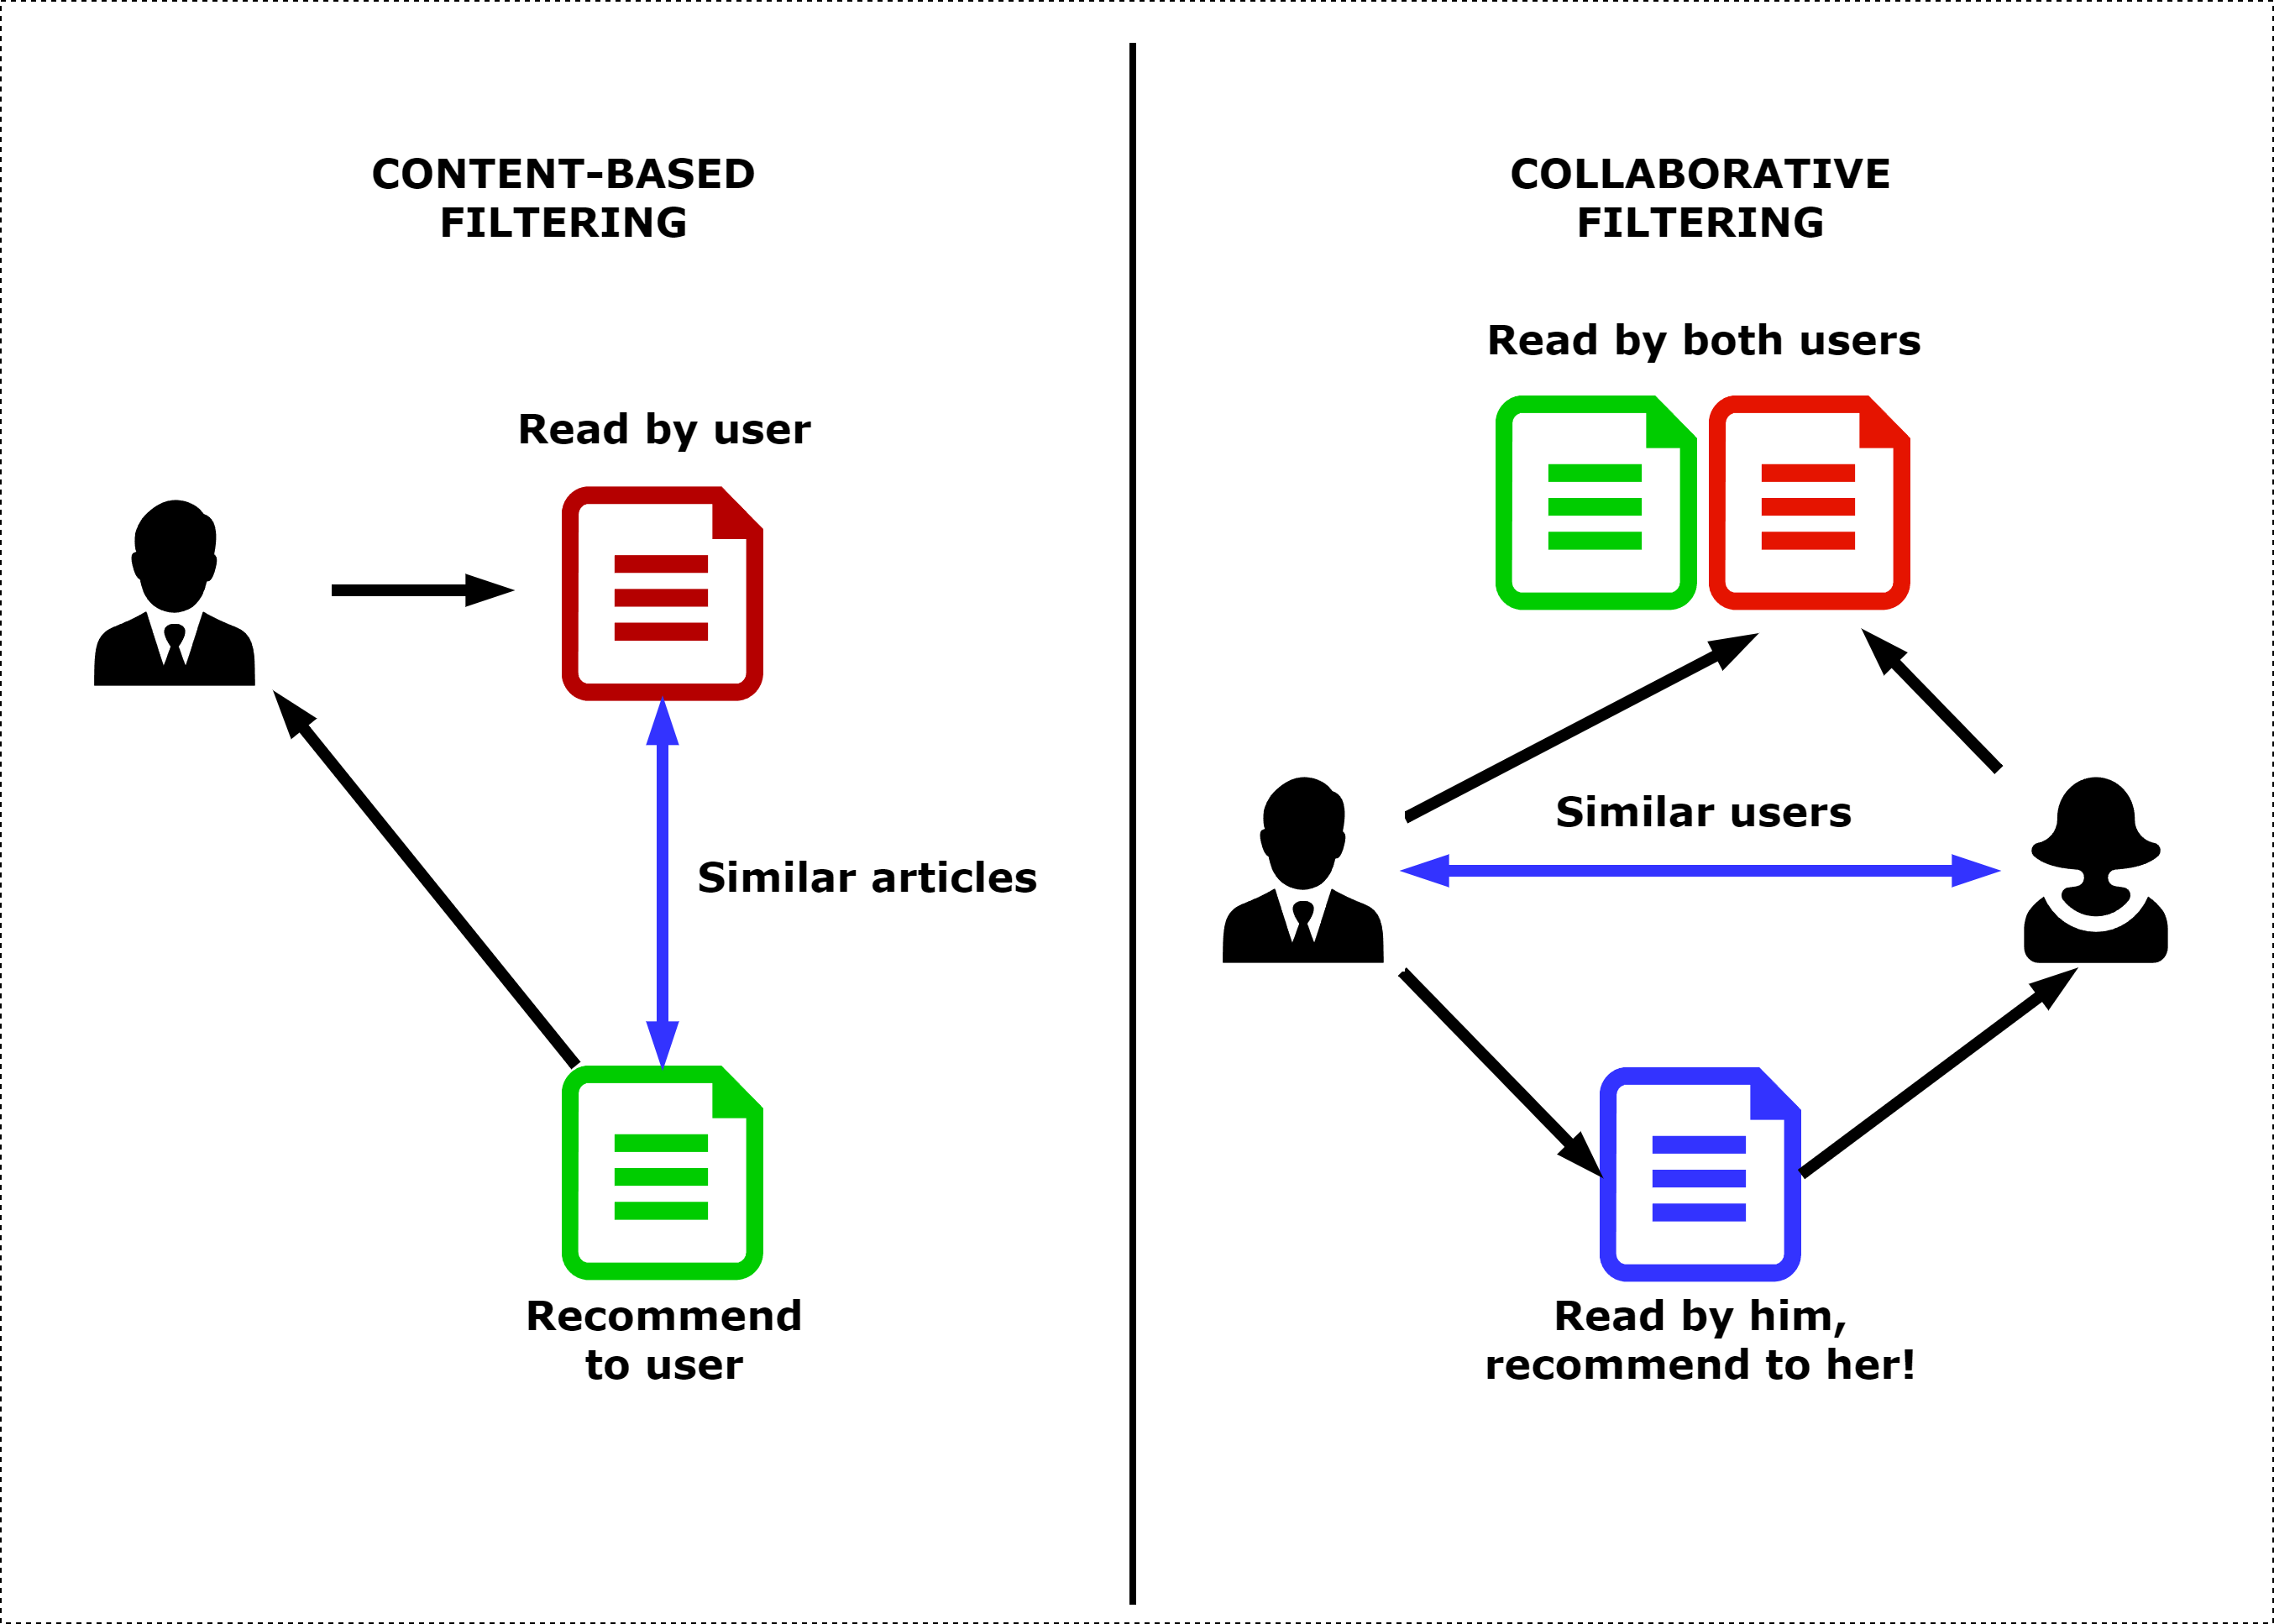
\includegraphics[width = 0.8\textwidth]{imgs/CF_CBF.png}
% %     \caption{Minh hoạ Lọc dựa trên nội dung và Lọc cộng tác}
% %     \label{fig:CF_CBF}
% % \end{figure}
% % \subsubsection{Lọc cộng tác}
% % Lọc cộng tác (Collaborative Filtering - CF) là một kỹ thuật phổ biến trong các hệ thống khuyến nghị, hoạt động dựa trên nguyên tắc "những người cùng sở thích sẽ có xu hướng thích những thứ tương tự nhau" (minh họa trong hình \ref{fig:CF_CBF}) \cite{cf2,cf3}. CF có thể được chia thành hai loại chính: dựa trên bộ nhớ (Memory-based) và dựa trên mô hình (Model-based).

% % \begin{enumerate}
% %     \item Lọc cộng tác dựa trên bộ nhớ (Memory-based): Phương pháp này tập trung vào việc tìm kiếm sự tương đồng giữa người dùng hoặc giữa các mục để đưa ra khuyến nghị. Ví dụ, trong kỹ thuật Lọc cộng tác người dùng-người dùng, hệ thống sẽ gợi ý các mục dựa trên những gì mà những người dùng có sở thích tương tự đã yêu thích hoặc đánh giá cao \cite{ncf1, ncf3}.
% %     \item Lọc cộng tác dựa trên mô hình (Model-based): Khác với phương pháp dựa trên bộ nhớ, cách tiếp cận này xây dựng một mô hình từ dữ liệu người dùng để dự đoán sở thích của họ. Một ví dụ điển hình là Phân tích ma trận (Matrix Factorization), một kỹ thuật phân tích dữ liệu đánh giá thành các yếu tố tiềm ẩn, đại diện cho sở thích của người dùng và đặc điểm của mục \cite{ncf2, ncf4}.
% % \end{enumerate}
% % \subsubsection{Lọc dựa trên nội dung}
% % Lọc Dựa trên nội dung (Content-based Filtering - CB) là một kỹ thuật khuyến nghị tập trung vào việc phân tích các đặc điểm nội tại của từng mục và sở thích của người dùng để đưa ra các đề xuất phù hợp. Điểm mấu chốt của phương pháp này nằm ở giả định rằng nếu người dùng yêu thích một mục cụ thể, họ cũng có xu hướng quan tâm đến những mục khác có nội dung tương đồng (như trong hình \ref{fig:CF_CBF}) \cite{cbf1,cbf2}. Ví dụ, nếu một người thường xuyên đọc các bài báo về học sâu, hệ thống có thể gợi ý cho họ những bài viết khác liên quan đến lĩnh vực này \cite{cbf, cbf1, cbf2}.


% % \subsubsection{Khuyến nghị tuần tự}
% % Gần đây, với sự tiến bộ trong các phương pháp học máy và học sâu, các hệ thống khuyến nghị tuần tự (Sequential Recommender Systems) đã nổi lên như một xu hướng mới, mang lại nhiều lợi ích và khả năng cải thiện trải nghiệm người dùng một cách đáng kể. Các mô hình khuyến nghị trong tuần tự tập trung vào thứ tự và ngữ cảnh của sản phẩm mà người dùng đã tương tác. Khoá luận này sẽ tập trung sử dụng mô hình khuyến nghị tuần tự đề xây dựng phương pháp đề xuất. Với hai mô hình cơ sở nổi bật được tập trung nghiên cứu là Self-Attentive Sequential Recommendation (SASRec) và Bidirectional Encoder Representations from Transformers for Recommendation (BERT4Rec).
% % \begin{figure}
% %     \centering
% %     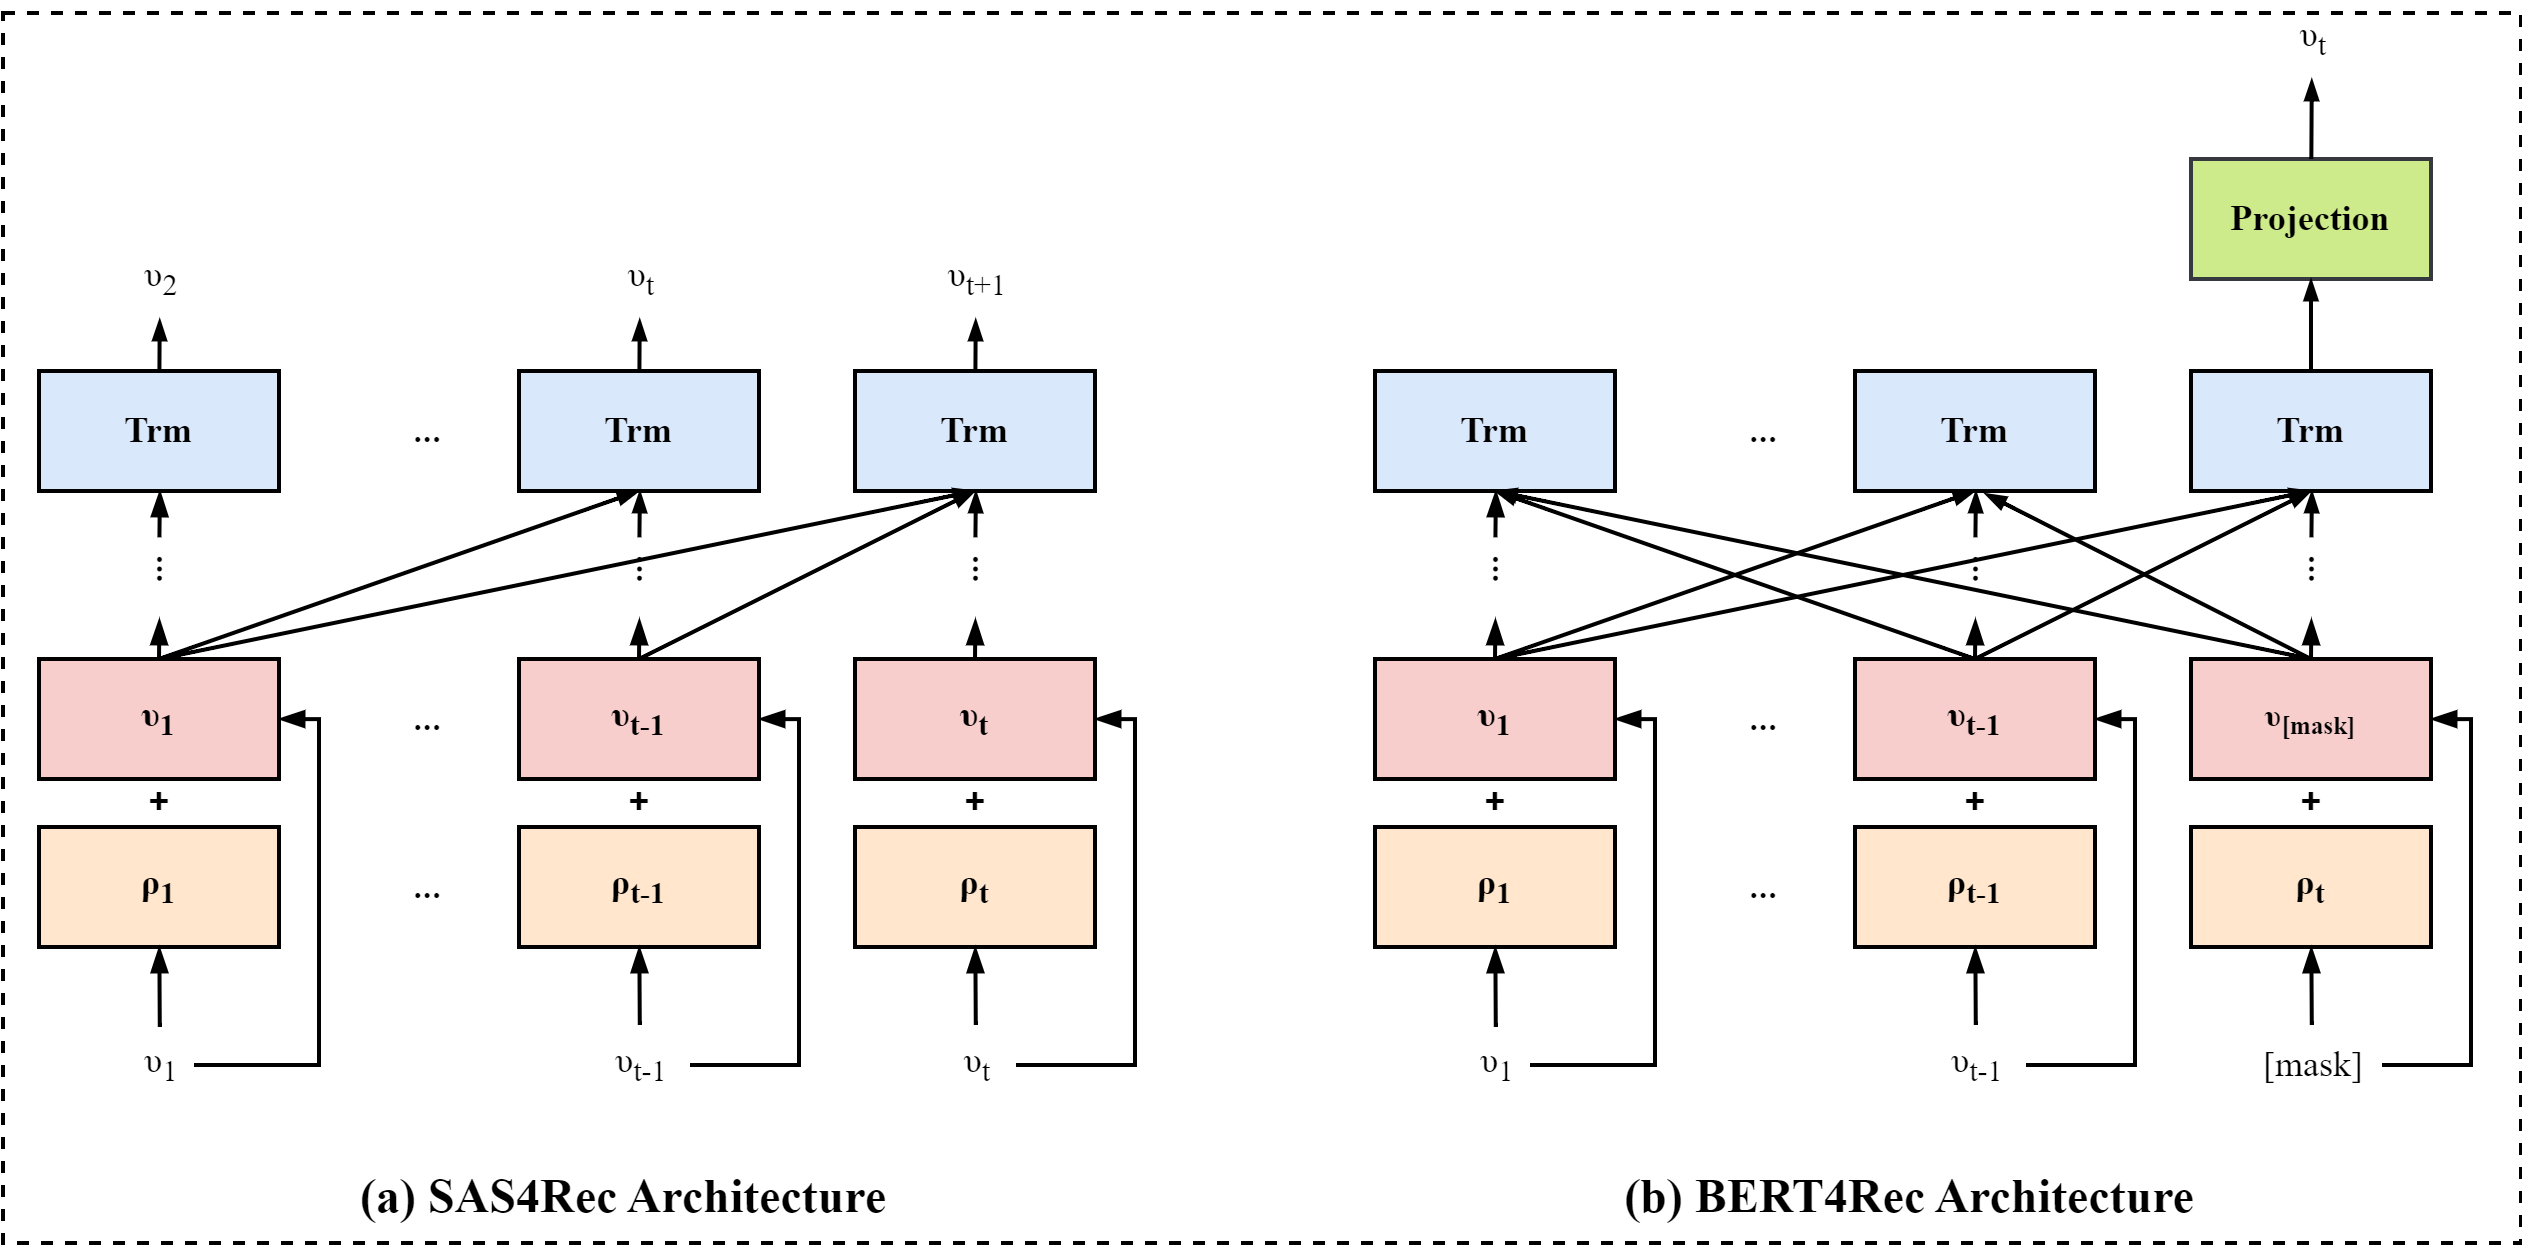
\includegraphics[width = \textwidth]{imgs/bert_sas_1.png}
% %     \caption{Kiến trúc của SASRec và BERT4Rec}
% %     \label{fig:bert_sas}
% % \end{figure}

% % \subsubsection{SASRec}
% % Được giới thiệu trong nghiên cứu \cite{sasrec}, SASRec là một trong những mô hình đầu tiên ứng dụng thành công Transformer vào bài toán khuyến nghị tuần tự. Như mô tả ở hình \ref{fig:bert_sas}a, điểm đặc biệt của SASRec nằm ở việc sử dụng cơ chế self-attention để nắm bắt các mối quan hệ phức tạp giữa các mục trong lịch sử tương tác của người dùng. Nhờ đó, mô hình có thể học được các biểu diễn phong phú và có ý nghĩa của từng mục, giúp dự đoán chính xác về mục tiếp theo mà người dùng có thể quan tâm. SASRec đã chứng minh được hiệu quả vượt trội so với các mô hình truyền thống như RNN và LSTM trong nhiều bài toán khuyến nghị tuần tự.
% % \subsubsection{BERT4Rec}
% % Được lấy cảm hứng từ mô hình BERT (Bidirectional Encoder Representations from Transformers), BERT4Rec được công bố trong nghiên cứu \cite{bert} với nhiệm vụ tận dụng khả năng của Transformer trong lĩnh vực hệ thống khuyến nghị. Khác với SASRec, ý tưởng chính của BERT4Rec là khai thác thông tin từ cả hai hướng (trước và sau) của chuỗi tương tác để xây dựng biểu diễn ngữ cảnh (như hình \ref{fig:bert_sas}b, cho phép mô hình nắm bắt được cả thông tin ngữ cảnh trước và sau của mỗi mục, từ đó hiểu rõ hơn về mối quan hệ giữa các mục và đưa ra các dự đoán chính xác hơn. BERT4Rec đã đạt được những kết quả ấn tượng trên nhiều tập dữ liệu, khẳng định vị thế của mình như một trong những mô hình hàng đầu trong lĩnh vực này.
% \subsubsection{Tổng kết}
% Tóm lại, các hệ thống khuyến nghị tuần tự đóng vai trò quan trọng trong việc mang đến trải nghiệm cá nhân hóa cho người dùng. Tuy nhiên, các mô hình này thường chỉ tập trung vào thông tin từ chuỗi hành vi của người dùng mà chưa tập trung vào việc khai thác thông tin đa chiều về các khóa học. Để giải quyết hạn chế này, nghiên cứu này đề xuất tích hợp HINs với BERT4Rec. Bằng cách khai thác các biểu diễn thực thể đa dạng thông qua HINs, mô hình kết hợp được cả đặc điểm nội dung và đặc điểm cấu trúc của các thực thể trong dữ liệu MOOCs. Sự tích hợp này hứa hẹn sẽ nâng cao đáng kể khả năng gợi ý các khái niệm kiến thức, nhờ vào việc tận dụng thông tin toàn diện từ nhiều nguồn khác nhau.

% \subsection{Các ứng dụng của lấy mẫu tiêu cực}
% Lấy mẫu tiêu cực (negative sampling) là một kỹ thuật lấy mẫu dữ liệu quan trọng, đặc biệt hiệu quả trong việc xử lý các tập dữ liệu mất cân bằng thường gặp trong các mô hình học máy như mạng nơ-ron và nhúng từ \cite{neg_1,neg_2}. Kỹ thuật này hoạt động bằng cách chọn lọc một tập hợp con các mẫu tiêu cực từ một phân phối xác định trước, thường sử dụng chiến lược lấy mẫu ngẫu nhiên. Tuy nhiên, việc lấy mẫu ngẫu nhiên không phải lúc nào cũng là lựa chọn tối ưu cho mọi nhiệm vụ. Trong lĩnh vực nhúng từ (như Word2Vec), negative sampling đã chứng minh được hiệu quả vượt trội trong việc giảm thiểu đáng kể khối lượng tính toán. Thay vì cập nhật trọng số dựa trên toàn bộ từ vựng, kỹ thuật này tập trung vào một tập hợp nhỏ các từ tiêu cực được lựa chọn cẩn thận, giúp tăng tốc độ huấn luyện và khả năng ứng dụng của mô hình nhúng từ, ngay cả với những bộ từ vựng lớn.

% Negative sampling có ứng dụng rộng rãi trong nhiều lĩnh vực, từ học máy, thị giác máy tính, xử lý ngôn ngữ tự nhiên đến khai thác dữ liệu và hệ thống gợi ý \cite{neg_1}. Có nhiều phương pháp negative sampling khác nhau, bao gồm static negative, hard negative và các phương pháp dựa trên GAN, mỗi phương pháp đều có ưu nhược điểm riêng. 
% Khoá luận này đề xuất một chiến lược lấy mẫu ngẫu nhiên mới với thông tin được tổng hợp bởi HINs. Nghiên cứu sẽ thực nghiệm để hiểu rõ tầm ảnh hưởng của việc áp dụng các chiến lược lấy mẫu ngẫu nhiên khác nhau khi xây dựng hệ thống khuyến nghị khoá học. Kết quả đánh giá sẽ cho thấy được rằng việc áp dụng chiến lược lấy mẫu ngẫu nhiên mà khoá luận đề xuất là tốt hơn so với các chiến lược được sử dụng trong các nghiên cứu trước đây như \cite{bert, sasrec, gru_ori}.

% \subsection{Mạng thông tin không đồng nhất}
% Mạng thông tin không đồng nhất (HINs) đã thu hút sự quan tâm lớn từ cộng đồng nghiên cứu do khả năng biểu diễn dữ liệu phong phú và đa dạng từ nhiều nguồn thông tin khác nhau. Các HINs không chỉ lưu trữ các loại đối tượng và liên kết khác nhau mà còn hỗ trợ các ứng dụng phân tích dữ liệu phức tạp, từ việc khai thác tri thức đến dự đoán và khuyến nghị. HINs là các mạng trong đó tồn tại nhiều loại đối tượng và liên kết, khác biệt với các mạng đồng nhất truyền thống nơi chỉ có một loại đối tượng và một loại liên kết duy nhất \cite{rlt_hin}. Cho phép HINs mô hình hóa mối quan hệ phức tạp giữa các thực thể khác nhau và hỗ trợ các ứng dụng trong nhiều lĩnh vực như mạng xã hội, khoa học dữ liệu, và y học. Khác với các mạng đồng nhất, nơi mà tất cả các đối tượng và liên kết đều cùng loại, HINs cung cấp một cấu trúc phong phú hơn, cho phép biểu diễn mối quan hệ phức tạp giữa các loại thực thể khác nhau \cite{rlt_hin2}. Các mạng đồng nhất thường không thể hiện được đầy đủ sự đa dạng và ngữ cảnh của dữ liệu, dẫn đến việc mất mát thông tin quan trọng khi mô hình hóa các hệ thống phức tạp.

% \subsubsection{Ưu điểm}
% \begin{itemize}
%     \item Biểu diễn thông tin phong phú: HINs có khả năng biểu diễn thông tin một cách chi tiết và đa dạng từ nhiều loại đối tượng và mối liên kết khác nhau, giúp cung cấp ngữ cảnh đầy đủ và chính xác hơn \cite{rlt_hin}.
    
%     \item Nâng cao khả năng phân tích: Khả năng khai thác các mối quan hệ đa dạng và gián tiếp giữa các đối tượng giúp HINs tăng cường khả năng phân tích và khai thác tri thức từ dữ liệu \cite{rlt_hin2}.
    
%     \item Cải thiện độ chính xác của khuyến nghị: Bằng cách tận dụng thông tin từ nhiều nguồn và mối quan hệ khác nhau, HINs giúp cải thiện đáng kể hiệu suất của các hệ thống khuyến nghị \cite{rlt_hin3}.
% \end{itemize}
% \subsubsection{Thách thức}
% \begin{itemize}
%     \item Độ phức tạp: Việc xây dựng và quản lý HINs đòi hỏi nhiều công sức và kỹ thuật hơn so với các mạng đồng nhất, do tính chất đa dạng và phức tạp của dữ liệu \cite{rlt_hin3}. Các phương pháp đặc biệt cần được phát triển để xử lý và khai thác hiệu quả dữ liệu từ HINs.
    
%     \item Khả năng mở rộng: Khả năng mở rộng của các mô hình HINs là một thách thức đáng kể do sự đa dạng và phức tạp của dữ liệu \cite{rlt_hin5}. Việc áp dụng HINs cho các tập dữ liệu lớn đòi hỏi các giải pháp tối ưu hóa và xử lý phân tán để đảm bảo hiệu suất và khả năng đáp ứng của mô hình.
% \end{itemize}

% HINs đại diện cho một bước tiến quan trọng trong việc khai thác và phân tích dữ liệu phức tạp. Nhờ khả năng biểu diễn và khai thác thông tin từ nhiều loại đối tượng và mối quan hệ, HINs đã mở ra nhiều cơ hội mới cho các ứng dụng phân tích dữ liệu và hệ thống khuyến nghị, đồng thời đặt ra những thách thức mới về mặt kỹ thuật và mô hình hóa.





% % Hệ thống gợi ý tuần tự trong MOOCs có khả năng xử lý hành vi theo thời gian của người dùng, tuy nhiên khả năng nắm bắt ngữ cảnh đa dạng còn hạn chế. Ngữ cảnh này bao gồm các khóa học, cấu trúc kiến thức, mối quan hệ tiền quyết, hồ sơ học viên và các thực thể liên quan khác. Để giải quyết vấn đề này, nghiên cứu gần đây đã tập trung vào việc áp dụng Mạng thông tin không đồng nhất (HIN) cho hệ thống gợi ý MOOCs.

% % HIN là loại mạng chứa nhiều loại nút và cạnh khác nhau, biểu diễn các mối quan hệ phức tạp trong dữ liệu. Chúng nắm bắt ý nghĩa sâu sắc của các đối tượng được cấu trúc và các kết nối trong mạng, cho phép phân tích và khai thác dữ liệu phức tạp hơn, cung cấp cái nhìn toàn diện về các cấu trúc và mối quan hệ ẩn giữ các thực thể\cite{hin_1}. Mặc dù HIN mang lại nhiều tiềm năng, việc áp dụng nó vào hệ thống gợi ý thực tiễn đặt ra nhiều thách thức. Một trong những thách thức chính là sự thưa thớt dữ liệu, nơi số lượng cạnh giữa các thực thể có thể không đủ để học các biểu diễn mạnh mẽ. Ngoài ra, việc thiết kế các phương pháp hiệu quả để tích hợp các nguồn dữ liệu đa dạng và các mối quan hệ phức tạp trong HINs có thể đòi hỏi tài nguyên tính toán đáng kể \cite{hin_2, hin_3, hin_4}.

% % Mô hình Heterogeneous Embedding for Recommendation (\textbf{HERec}) \cite{hin_5} đã cho thấy tiềm năng trong việc giải quyết những hạn chế này. HERec sử dụng các kỹ thuật nhúng để học các biểu diễn vector học viên, khóa học và các thực thể khác trong HINs. Biểu diễn mối quan hệ tự nhiên giữa các thực thể dựa trên kết nối của chúng trong mạng, cho phép HERec mô hình hóa hiệu quả các tương tác phức tạp giữa học viên, khóa học, khái niệm kiến thức và các khía cạnh quan trọng khác trong hệ sinh thái MOOCs. Cụ thể, HERec tận dụng các kỹ thuật dựa trên meta-path để khám phá các đường dẫn khác nhau trong HIN kết nối học viên với khóa học. Bằng cách xem xét những đường dẫn đa dạng này, HERec có thể nắm bắt được ngữ cảnh xung quanh các tương tác giữa học viên và khóa học, giúp cho các gợi ý được cá nhân hóa và phù hợp hơn cho người học.

% % Sự xuất hiện của mạng không đồng nhất và mô hình \textbf{HERec} đại diện cho một bước tiến đáng kể trong các hệ thống gợi ý MOOCs. Bằng cách nắm bắt mạng lưới phức tạp của các mối quan hệ trong hệ sinh thái MOOCs, HINs cung cấp một ngữ cảnh phong phú hơn để hiểu hành vi của người dùng. Kết hợp với hiệu quả của HERec trong việc học các biểu diễn có ý nghĩa từ mạng này, nó mở ra con đường phát triển các hệ thống gợi ý cá nhân hóa và tinh vi hơn cho các nền tảng MOOCs.

\section{Deep learning}

Sự trỗi dậy của học sâu (deep learning) trong những năm gần đây đã mở ra những hướng tiếp cận mới để khai thác tri thức từ các bộ dữ liệu lớn. Trong lĩnh vực giáo dục, Mạng nơ-ron nhân tạo (ANN) là một trong những kiến trúc nền tảng được ứng dụng rộng rãi nhất để phân tích hành vi người học. Với cấu trúc nhiều lớp mô phỏng não bộ, ANN thể hiện khả năng xử lý hiệu quả dữ liệu quy mô lớn. Các ứng dụng của nó rất đa dạng, từ việc dự báo kết quả học tập, xác định các hành vi bất thường có thể dẫn đến việc bỏ học, cho đến gợi ý các lộ trình học tập được cá nhân hóa \cite{waheed2020predicting, coelho2017deep}.

Bên cạnh ANN, các kiến trúc sâu hơn như Mạng Nơ-ron Sâu (DNNs) và đặc biệt là các mô hình lai ghép như CNN-LSTM đã chứng tỏ được hiệu quả vượt trội trong giai đoạn 2019-2023. Các kỹ thuật như Mạng tích chập (CNN) và Mạng bộ nhớ dài-ngắn (LSTM) khi được kết hợp có khả năng xử lý hiệu quả các dữ liệu giáo dục vốn có tính đa chiều và phi tuyến tính. Nhiều nghiên cứu trong giai đoạn này đã báo cáo độ chính xác trên 90\%, qua đó củng cố mạnh mẽ niềm tin về tiềm năng của học sâu trong việc dự đoán hành vi và kết quả học tập \cite{albreiki2021systematic}.

Sức mạnh kiến trúc lai CNN-LSTM nằm ở sự tổng hợp của hai năng lực bổ trợ cho nhau: Năng lực xử lý thông tin không gian của CNN và thông tin thời gian của LSTM. Nhờ đó, mô hình này có thể phân tích hiệu quả các dữ liệu học tập chứa cả yếu tố không gian (ví dụ: các loại tương tác khác nhau) và yếu tố thời gian (trình tự và thời điểm của các hành động đó). Điều này hữu ích cho các nhiệm vụ như dự báo điểm số, nhận diện nguy cơ bỏ học và hỗ trợ các quyết định sư phạm \cite{aljaloud2022deep}.

Để xử lý hiệu quả hơn nữa dữ liệu dạng chuỗi thời gian vốn rất phổ biến trong giáo dục trực tuyến, kiến trúc LSTM xếp chồng nhiều lớp (stacked LSTM), chẳng hạn như mô hình 4 lớp, đã được đề xuất. Việc xếp chồng các lớp LSTM cho phép mô hình học được các biểu diễn trừu tượng ở mức độ cao hơn, từ đó nắm bắt được các mẫu hành vi phức tạp và dài hạn qua nhiều phiên học. Do vậy, kiến trúc này tỏ ra rất hiệu quả trong việc phân tích quá trình học tập và dự báo các kết quả trong tương lai \cite{kukkar2023prediction, ren2023prediction}.

Một bước tiến xa hơn trong việc phân tích dữ liệu tuần tự là việc áp dụng LSTM hai chiều (BiLSTM), một kiến trúc có khả năng khai thác thông tin từ cả quá khứ và tương lai của chuỗi. Khi được tích hợp với cơ chế chú ý (attention mechanism), BiLSTM càng cho thấy ưu thế vượt trội. Cơ chế chú ý giúp mô hình tập trung vào những thời điểm hoặc hành vi quan trọng nhất trong chuỗi, những yếu tố có ảnh hưởng quyết định đến kết quả cuối cùng. Sự kết hợp này đã mang lại độ chính xác cao hơn đáng kể trong việc phân tích hành vi, mở đường cho việc thiết kế các hệ thống cảnh báo sớm và hỗ trợ học tập thông minh \cite{yousafzai2021student}.

Tóm lại, bức tranh ứng dụng học sâu trong lĩnh vực khai phá dữ liệu giáo dục rất đa dạng và không ngừng phát triển. Các kiến trúc từ ANN, DNN, CNN-LSTM, stacked LSTM, cho đến BiLSTM với cơ chế chú ý, đã tạo thành một bộ công cụ mạnh mẽ. Chúng không những là các công cụ dự đoán hiệu quả mà còn là phương tiện để khám phá bản chất phức tạp, đa chiều của hành vi học tập trong kỷ nguyên số.

% Một trong những mô hình học sâu đã nổi lên và khá nổi tiếng trong nghiên cứu hành vi người học là mạng nơ-ron nhân tạo (Artificial Neural Networks – ANN). Cơ chế ANNs khá giống cơ chế hoạt động của não bộ con người nhờ các lớp nơ-ron nhân tạo, thường bao gồm ba lớp cơ bản: lớp đầu vào, lớp ẩn và lớp đầu ra. ANNs có khả năng xử lý dữ liệu lớn và có hiệu quả trong việc dự đoán kết quả học tập, phát hiện hành vi bất thường của các học viên có nguy cơ không hoàn thành khóa học và gợi ý những lộ trình học tập tối ưu hóa cho từng cá nhân \cite{waheed2020predicting, coelho2017deep}.

% Bên cạnh ANNs, Deep Neural Networks – DNNs và các kiến trúc kết hợp như CNN-LSTM cũng được áp dụng rộng rãi trong bài toán giáo dục, đặc biệt trong giai đoạn 2019-2023. Sức mạnh của các kỹ thuật như mạng tích chập (Convolutional Neural Networks – CNNs), mạng ghi nhớ dài hạn (Long Short-Term Memory – LSTM) và các mô hình kết hợp để xử lý dữ liệu giáo dục có tính chất đa chiều và phi tuyến đã được nghiên cứu rất nhiều trong khoảng thời gian này. Những mô hình này thường đạt được độ chính xác rất cao, trong nhiều trường hợp vượt mốc 90\%, góp phần củng cố niềm tin vào khả năng áp dụng học sâu trong dự đoán học lực và hành vi học tập \cite{albreiki2021systematic}.

% Mô hình CNN-LSTM là sự kết hợp giữa khả năng trích xuất đặc trưng không gian của CNN và khả năng ghi nhớ tuần tự của LSTM. CNN-LSTM xử lý dữ liệu học tập có cả yếu tố không gian (chẳng hạn như các loại hành vi học tập khác nhau) và yếu tố thời gian (thứ tự và thời điểm thực hiện hành vi) rất hiệu quả. Chính vì đó, nó phục vụ cho các nhiệm vụ như dự đoán điểm số, xác định nguy cơ bỏ học và hỗ trợ ra quyết định giảng dạy \cite{aljaloud2022deep}.

% Đặc biệt, kiến trúc LSTM xếp chồng nhiều lớp (stacked LSTM), tiêu biểu là mô hình 4-layer-stacked, được thiết kế để khai thác dạng dữ liệu chuỗi thời gian thường phổ biến trong các hệ thống học tập trực tuyến. Việc xếp chồng nhiều lớp LSTM giúp mô hình có thể học được các đặc trưng trừu tượng hơn, đại diện cho mối liên hệ phức tạp giữa các hành vi học tập kéo dài qua nhiều phiên học.\cite{kukkar2023prediction, ren2023prediction}.

% Không dừng lại ở đó, các mô hình học sâu tiên tiến hơn như LSTM hai chiều (Bidirectional LSTM – BiLSTM) được quan tâm nhiều hơn nhờ khả năng khai thác thông tin từ cả quá khứ lẫn tương lai trong chuỗi thời gian. Khi kết hợp với cơ chế chú ý (attention mechanism), BiLSTM cho thấy ưu thế trong việc trích xuất biểu diễn từ dữ liệu chuỗi. Việc tích hợp BiLSTM với attention đã mang lại kết quả vô cùng khả quan, từ đó mở ra tiềm năng tích hợp vào các hệ thống dự đoán thông minh\cite{yousafzai2021student}.

% Tóm lại, Các kiến trúc như ANN, DNN, CNN-LSTM, stacked LSTM, và BiLSTM kết hợp với attention không chỉ đóng vai trò là công cụ dự đoán hiệu quả, mà còn góp phần quan trọng trong việc khám phá bản chất phức tạp và đa chiều của hành vi học tập trong môi trường số. Việc vận dụng những mô hình này một cách linh hoạt và sáng tạo sẽ là chìa khóa để giải quyết bài toán tỷ lệ bỏ học và cải thiện tỷ lệ hoàn thành các khóa học trực tuyến.
\chapter{Cơ sở lý thuyết}
\label{chap:chap3}

\section{Học sâu (Deep Learning)}
\subsection{Giới thiệu}
Về mặt kiến trúc, \textbf{Học sâu} được xây dựng dựa trên các mạng nơ-ron nhân tạo có chiều sâu, bao gồm nhiều lớp ẩn xếp chồng lên nhau. Mặc dù là một nhánh của Học máy, điểm ưu việt của Học sâu đến từ khả năng tự động khám phá và biểu diễn phân cấp cho dữ liệu. Điều này có nghĩa là mô hình có thể tự học từ các đặc trưng cơ bản đến các đặc trưng trừu tượng hơn. Năng lực này đặc biệt hữu ích khi xử lý các bộ dữ liệu lớn và phức tạp, chẳng hạn như dữ liệu đa phương thức trong môi trường MOOCs.

Sự tăng trưởng mạnh mẽ của dữ liệu trong những năm gần đây, kết hợp với những tiến bộ vượt bậc của năng lực xử lý tính toán, đã tạo ra một môi trường lý tưởng cho các mô hình học sâu phát triển. Học sâu đã chứng tỏ hiệu quả trong nhiều lĩnh vực. Điểm khác biệt mang tính cách mạng của Học sâu so với các phương pháp truyền thống là khả năng tự động học hỏi đặc trưng (feature learning), có thể phát hiện các mối quan hệ và mẫu tiềm ẩn trong dữ liệu một cách hiệu quả hơn.

\subsection{Các Kiến trúc Học sâu cho Dữ liệu Chuỗi}
Bản chất tuần tự của hành vi người học trên các nền tảng MOOCs đòi hỏi việc sử dụng các pipeline học sâu được thiết kế chuyên biệt cho dữ liệu chuỗi thời gian.

\begin{itemize}
    \item \textbf{Mạng nơ-ron hồi quy (Recurrent Neural Networks - RNNs)}\cite{SHERSTINSKY2020132306}:
    \begin{itemize}
        \item \textbf{Nguyên lý hoạt động:} Đặc trưng cốt lõi của RNN là khả năng nắm bắt sự phụ thuộc tuần tự trong dữ liệu. Mô hình thực hiện điều này bằng cách sử dụng một bộ nhớ nội tại (trạng thái ẩn) để lưu giữ thông tin từ các bước trước đó, tạo ra một ngữ cảnh cho việc xử lý dữ liệu ở bước hiện tại. 
        \item \textbf{Cơ chế:} Tại mỗi bước thời gian $t$, đầu ra được ký hiệu là $h_t$, được xác định dựa trên sự kết hợp giữa đầu vào hiện tại $x_t$ và trạng thái ẩn từ bước thời gian trước đó $h_{t-1}$. Từ đó, RNN có thể xử lý được dữ liệu tuần tự. Quá trình này được mô hình hóa theo công thức:

\[
h_t = f(W_{xh}x_t + W_{hh}h_{t-1} + b_h)
\]

trong đó:
\begin{itemize}
    \item $W_{xh}$ là ma trận trọng số kết nối đầu vào với lớp ẩn.
    \item $W_{hh}$ là ma trận trọng số kết nối trạng thái ẩn trước với trạng thái ẩn hiện tại.
    \item $b_h$ là vector độ lệch (bias).
    \item $f$ là hàm kích hoạt phi tuyến, thường là $\tanh$ hoặc ReLU.
\end{itemize}
        \item \textbf{Hạn chế:} Các kiến trúc RNN truyền thống bộc lộ yếu điểm khi xử lý các chuỗi dài do phải đối mặt với hai vấn đề nghiêm trọng: \textbf{suy biến gradient (vanishing gradient)} và \textbf{bùng nổ gradient (exploding gradient)}. Các hiện tượng này cản trở khả năng của mô hình trong việc học và ghi nhớ các mối phụ thuộc kéo dài qua nhiều bước thời gian. 

    \end{itemize}

    \item \textbf{Mạng bộ nhớ dài-ngắn (LSTMs)}\cite{10.1162/neco_a_01199}:
    \begin{itemize}
        \item \textbf{Giải pháp cho RNN:} LSTM là một kiến trúc cải tiến, được thiết kế đặc biệt để giải quyết các hạn chế cố hữu của RNN. Nhờ cấu trúc đặc biệt, LSTM có khả năng lưu giữ và tận dụng các mối quan hệ phụ thuộc dài hạn một cách hiệu quả, điều mà các mạng RNN truyền thống thường gặp khó khăn trong việc xử lý.

        \item \textbf{Kiến trúc Cổng:} LSTM đạt được điều này thông qua một kiến trúc phức tạp hơn với các "cổng" (gates) nội bộ kiểm soát luồng thông tin vào và ra khỏi một "ô nhớ" (cell state). Các cổng này bao gồm:
        \begin{itemize}
            \item \textbf{Cổng quên (Forget Gate):} Xác định phần thông tin nào trong trạng thái ô nhớ cũ cần được lãng quên hoặc loại bỏ.
            \item \textbf{Cổng đầu vào (Input Gate):} Kiểm soát việc cập nhật thông tin mới vào trạng thái ô nhớ.
            \item \textbf{Cổng đầu ra (Output Gate):} Điều tiết thông tin nào từ trạng thái ô nhớ sẽ được sử dụng để tạo ra kết quả đầu ra tại bước thời gian hiện tại.
        \end{itemize}
        \item \textbf{Ưu điểm:} Khả năng kiểm soát thông tin chi tiết này cho phép LSTM ghi nhớ thông tin quan trọng qua nhiều bước thời gian, làm cho chúng trở nên mạnh mẽ trong việc mô hình hóa các chuỗi hành vi học tập phức tạp.
        \item \textbf{Ứng dụng:} Trong khuôn khổ khóa luận này, chúng tôi triển khai mô hình \textbf{LSTM xếp chồng 4 lớp (4-layer stacked LSTM)}. Kiến trúc xếp chồng cho phép mô hình học các biểu diễn dữ liệu ở nhiều cấp độ trừu tượng. Nhờ đó, nó có thể phân tích các mẫu hành vi ở nhiều quy mô khác nhau: từ các tương tác tức thời ở cấp độ vi mô (như một cú nhấp chuột) cho đến các xu hướng học tập tổng thể kéo dài ở cấp độ vĩ mô (như chiến lược học tập của người dùng trong cả khóa học). 
    \end{itemize}

    \item \textbf{Mạng đơn vị hồi tiếp có cổng (Gated Recurrent Unit - GRUs)}\cite{MIM2023119419}:
    \begin{itemize}
        \item \textbf{Một biến thể tối ưu của LSTM:} GRU là một kiến trúc tinh gọn hơn của LSTM, được phát triển nhằm cải thiện hiệu quả tính toán trong khi vẫn duy trì được năng lực nắm bắt các mối phụ thuộc dài hạn trong dữ liệu chuỗi.
        
        \item \textbf{Kiến trúc được đơn giản hóa:} GRU giảm độ phức tạp so với LSTM bằng cách chỉ sử dụng hai cơ chế cổng: \textbf{cổng cập nhật (update gate)} và \textbf{cổng đặt lại (reset gate)}. Việc giảm số lượng tham số này không chỉ giúp rút ngắn đáng kể thời gian huấn luyện mà trong nhiều bài toán cụ thể, còn có thể mang lại hiệu suất tương đương hoặc thậm chí vượt trội hơn so với LSTM.
        
        \item \textbf{Lựa chọn chiến lược cho dữ liệu lớn:} Trong bối cảnh làm việc với các bộ dữ liệu quy mô lớn như MOOCs, GRU nổi lên như một giải pháp thay thế hiệu quả, giúp đạt được sự cân bằng tối ưu giữa độ chính xác của mô hình và chi phí tài nguyên tính toán.
    \end{itemize}

    \item \textbf{Mạng LSTM hai chiều (BiLSTM)}\cite{singla2022ensemble}:
    \begin{itemize}
        \item \textbf{Khai thác ngữ cảnh toàn diện:} BiLSTM là một kiến trúc cải tiến của LSTM, cho phép mô hình xử lý chuỗi đầu vào từ quá khứ đến hiện tại (forward pass) và từ tương lai về hiện tại (backward pass).
        \item \textbf{Cách hoạt động:} bao gồm hai lớp LSTM riêng biệt: một lớp xử lý chuỗi dữ liệu theo chiều thời gian tiến (\textit{forward}), và lớp còn lại xử lý cùng chuỗi theo chiều thời gian ngược lại (\textit{backward}). Các đầu ra tại mỗi bước thời gian từ hai chiều được kết hợp (thường thông qua phép nối vector) để tạo ra biểu diễn ngữ cảnh đầy đủ, phản ánh thông tin từ cả quá khứ lẫn tương lai.
        \item \textbf{Lợi ích:}  BiLSTM có thể nắm bắt được hành vi của người học một cách tổng quát hơn, ví dụ như một hành động ở giữa khóa học có thể được hiểu rõ hơn khi biết hành động dẫn đến nó và hành động xảy ra sau đó. 
    \end{itemize}
\end{itemize}

\section{Mạng nơ-ron đồ thị (GNNs)}

\subsection{Tổng quan về lý thuyết đồ thị}
\textbf{Lý thuyết đồ thị} là một lĩnh vực trọng yếu trong toán học rời rạc, chuyên nghiên cứu các đối tượng được gọi là đồ thị. Về mặt hình thức, một \textbf{đồ thị (Graph)} $G = (V, E)$ được định nghĩa bởi một tập hợp hữu hạn các \textbf{đỉnh (Vertices/Nodes)} $V$ và một tập hợp các \textbf{cạnh (Edges)} $E$, với mỗi cạnh biểu diễn một mối liên kết giữa một cặp đỉnh. Các cạnh này có thể là có hướng (directed) hoặc vô hướng (undirected), và có thể được gán một \textbf{trọng số (weighted)} để thể hiện cường độ của mối liên kết đó.

Trong các hệ thống phức tạp như MOOCs, các cấu trúc dữ liệu truyền thống như dạng bảng hay chuỗi thường không đủ để nắm bắt được các mối quan hệ nội tại phức tạp. Lý thuyết đồ thị cung cấp một phương pháp biểu diễn tự nhiên và mạnh mẽ cho các mối quan hệ này. Ví dụ, ta có thể mô hình hóa dữ liệu MOOCs như sau:
\begin{itemize}
    \item Mỗi \textbf{người học} là một đỉnh, còn cạnh thể hiện sự tương tác xã hội (ví dụ, trên diễn đàn) hoặc sự tương đồng trong hành vi học tập.
    \item Mỗi \textbf{khóa học} là một đỉnh, và cạnh biểu thị sự liên quan về mặt chủ đề giữa các khóa học.
    \item Các đỉnh bao gồm cả \textbf{người học} và \textbf{khóa học}, trong đó cạnh đại diện cho hành vi ghi danh hoặc các tương tác khác.
    \item Các \textbf{video}, \textbf{bài tập}, hoặc \textbf{khái niệm học tập} là các đỉnh, và cạnh mô tả mối liên kết về cấu trúc và trình tự bên trong một khóa học.
\end{itemize}


\subsection{Mạng nơ-ron đồ thị (GNNs)}
GNNs là một lớp các mô hình học sâu được phát triển chuyên biệt để làm việc với dữ liệu có cấu trúc phi Euclidean, mà đồ thị là một dạng điển hình. Trong khi các kiến trúc như Mạng nơ-ron tích chập (CNNs) được tối ưu cho dữ liệu có cấu trúc dạng lưới (ví dụ: hình ảnh) và Mạng nơ-ron hồi quy (RNNs) phù hợp với dữ liệu dạng chuỗi, GNNs lại có khả năng học các vector biểu diễn (embedding) cho các đỉnh và cạnh. Năng lực này có được thông qua việc tổng hợp thông tin từ các đỉnh kề và khai thác cấu trúc liên kết toàn cục của đồ thị.

Ý tưởng cốt lõi của GNNs là \textbf{lan truyền thông tin (message passing)}: một đỉnh sẽ cập nhật biểu diễn của mình bằng cách tổng hợp thông tin không chỉ từ các đỉnh lân cận mà còn từ chính bản thân nó. Quá trình truyền và tích lũy thông tin này được lặp lại qua nhiều lớp, giúp thông tin lan rộng dần trên toàn bộ cấu trúc đồ thị. Nhờ đó, mỗi đỉnh dần xây dựng được một biểu diễn giàu ngữ cảnh, phản ánh không chỉ đặc trưng cục bộ mà còn cả cấu trúc toàn cục xung quanh nó.

\subsection{Mạng nơ-ron tích chập trên đồ thị (GCNs)}
\textbf{Mạng nơ-ron tích chập trên đồ thị (GCNs)} là một trong những kiến trúc GNN có tầm ảnh hưởng và được ứng dụng rộng rãi nhất. Ý tưởng cốt lõi của GCN là khái quát hóa phép toán tích chập (convolution), vốn rất thành công trên dữ liệu có cấu trúc Euclidean (như ảnh, chuỗi), để có thể áp dụng được cho dữ liệu có cấu trúc đồ thị bất quy tắc.

Về nguyên tắc, mỗi lớp của mạng GCN thực hiện một quá trình tổng hợp và biến đổi đặc trưng. Cụ thể, biểu diễn mới của mỗi đỉnh được tạo ra bằng cách tổng hợp các biểu diễn từ tập đỉnh lân cận của nó, sau đó áp dụng một phép biến đổi tuyến tính (thông qua một ma trận trọng số có thể học được) và một hàm kích hoạt phi tuyến. Nhờ cơ chế này, GCN có khả năng học được các biểu diễn không chỉ dựa trên đặc tính nội tại của đỉnh mà còn dựa trên ngữ cảnh được cung cấp bởi các đỉnh lân cận.


Công thức của một lớp GCN thường được biểu diễn như sau \cite{berg2017graph}:
$$H^{(l+1)} = \sigma(\tilde{D}^{-\frac{1}{2}}\tilde{A}\tilde{D}^{-\frac{1}{2}}H^{(l)}W^{(l)})$$
Trong đó:
\begin{itemize}
    \item $H^{(l)}$: Ma trận đặc trưng của các đỉnh ở lớp thứ $l$. $H^{(0)}$ thường là ma trận đặc trưng ban đầu của các đỉnh.
    \item $\tilde{A} = A + I$: Ma trận kề của đồ thị ($A$) được bổ sung ma trận đơn vị ($I$). Việc thêm $I$ đảm bảo rằng thông tin của chính đỉnh đó cũng được đưa vào quá trình tổng hợp.
    \item $\tilde{D}$: Ma trận bậc (degree matrix) của $\tilde{A}$. Đây là ma trận đường chéo mà mỗi phần tử $\tilde{D}_{ii}$ là tổng các giá trị trong hàng $i$ của $\tilde{A}$.
    \item $\tilde{D}^{-\frac{1}{2}}\tilde{A}\tilde{D}^{-\frac{1}{2}}$: Toán tử chuẩn hóa đối xứng, giúp ổn định quá trình huấn luyện và tránh các vấn đề về tỷ lệ.
    \item $W^{(l)}$: Ma trận trọng số huấn luyện của lớp thứ $l$, được học trong quá trình huấn luyện mô hình.
    \item $\sigma$: Hàm kích hoạt phi tuyến (ví dụ: ReLU, Sigmoid), đưa tính phi tuyến vào mô hình.
\end{itemize}

\textbf{Ứng dụng của GCNs trong làm giàu dữ liệu cho MOOCs:}
Trong khóa luận này, GCNs được khai thác như một công cụ mạnh mẽ để \textbf{làm giàu dữ liệu} trên các nền tảng MOOCs, đặc biệt là trong việc \textbf{điền khuyết giá trị (imputation)} cho các thông tin bị thiếu. Ý tưởng là khai thác mối quan hệ giữa các thực thể học tập như người học, khóa học và trường học và biến nó thành một đồ thị. Trong trường hợp một số đặc trưng của các thực thể này bị thiếu (chẳng hạn như điểm của một bài kiểm tra hoặc thời lượng xem video), GCN có thể tận dụng thông tin từ cấu trúc kết nối trong đồ thị để suy luận và ước lượng giá trị bị thiếu.

\begin{enumerate}
    \item \textbf{Mô hình hóa dữ liệu thành đồ thị:} Người học, khóa học, và các hành vi học tập được ánh xạ thành các đỉnh. Các mối quan hệ (ví dụ: người học $X$ đã đăng ký khóa học $Y$, người học $X$ đang học tại trường $Z$ khi học khóa học $Y$) được biểu diễn bằng các cạnh. Các đặc trưng ban đầu của các đỉnh (ví dụ: thông tin nhân khẩu học người học, đặc trưng hành vi người học) là đầu vào cho GCN.
    \item \textbf{Lan truyền thông tin và học biểu diễn:} GCN sẽ thực hiện quá trình lan truyền thông tin qua các lớp. Mỗi đỉnh sẽ lấy thông tin từ chính nó và các cạnh xung quanh. Nhờ vậy, các biểu diễn (embedding) của từng đỉnh có khả năng phản ánh ngữ cảnh xung quanh cũng như mối quan hệ với các đỉnh khác trong đồ thị, góp phần nâng cao chất lượng thông tin mà mô hình học được.

    \item \textbf{Suy luận giá trị thiếu:} Khi huấn luyện, GCN học cách ánh xạ các đặc trưng có sẵn của một đỉnh và các đỉnh lân cận thành một biểu diễn tổng hợp. Biểu diễn này sau đó có thể được sử dụng bởi một lớp đầu ra để dự đoán các giá trị đặc trưng bị thiếu. Chẳng hạn, nếu một người học không có dữ liệu về "thời gian xem video của khóa học X", GCN có thể dựa vào các người học tương tự (trên đồ thị) đã học khóa học X, hoặc dựa vào thời gian xem video khác mà người học đó đã xem từ các khóa học khác để suy luận giá trị bị thiếu này.
    \item \textbf{Nâng cao chất lượng dữ liệu đầu vào:} Việc bổ sung và hoàn thiện các đặc trưng còn thiếu giúp cho các mô hình học sâu kế tiếp (chẳng hạn như RNN, LSTM, GRU hay BiLSTM) dễ dàng học hỏi và hoạt động. Nhờ đó, khả năng mô hình hóa hành vi người học và dự đoán khả năng hoàn thành khóa học được cải thiện đáng kể.

\end{enumerate}

\section{Kỹ thuật làm giàu dữ liệu (Data Enrichment)}

\subsection{Định nghĩa}
\textbf{Làm giàu dữ liệu (Data Enrichment)} là một tập hợp các kỹ thuật nhằm gia tăng giá trị và độ tin cậy của một bộ dữ liệu. Quá trình này bao gồm việc tích hợp thêm các thông tin mới từ các nguồn bên ngoài, suy luận các đặc trưng tiềm ẩn, hoặc điền khuyết các giá trị bị thiếu. Trong bối cảnh các hệ thống phức tạp như MOOCs, nơi tình trạng dữ liệu không đầy đủ và thiếu nhất quán thường xuyên xảy ra, việc làm giàu dữ liệu được xem là một bước tiền xử lý mang tính chiến lược và không thể thiếu.

Các vai trò chính của quá trình làm giàu dữ liệu bao gồm:
\begin{itemize}
    \item \textbf{Hoàn thiện và nâng cao chất lượng dữ liệu:} Vai trò cơ bản nhất là khắc phục các điểm yếu cố hữu của dữ liệu thô, chẳng hạn như giảm thiểu nhiễu và bổ sung các giá trị bị thiếu, từ đó tạo ra một bộ dữ liệu sạch và toàn vẹn hơn.
    
    \item \textbf{Tối ưu hóa hiệu năng của mô hình:} Chất lượng dữ liệu đầu vào có mối tương quan trực tiếp đến hiệu suất của các mô hình học máy và học sâu. Một bộ dữ liệu đã được làm giàu sẽ cung cấp một nền tảng vững chắc hơn, giúp mô hình học được các mẫu quy luật chính xác hơn và đưa ra các dự đoán đáng tin cậy hơn.
    
    \item \textbf{Kiến tạo đặc trưng mới (Feature Engineering):} Bằng cách kết hợp dữ liệu từ nhiều nguồn hoặc khai thác các mối quan hệ cấu trúc, quá trình này cho phép tạo ra các đặc trưng mới có giá trị. Các đặc trưng này có thể cung cấp những góc nhìn sâu sắc mà dữ liệu gốc không thể hiện được, từ đó mang lại giá trị gia tăng đáng kể cho mô hình.
\end{itemize}

\subsection{Các phương pháp điền khuyết dữ liệu}
Để làm cơ sở so sánh, phần này sẽ tổng quan một số phương pháp xử lý dữ liệu thiếu truyền thống thường được áp dụng trong các nghiên cứu trước đây:
\begin{itemize}
    \item \textbf{Phương pháp loại bỏ (Listwise/Casewise Deletion)} \cite{Pepinsky_2018}: Đây là cách tiếp cận trực tiếp nhất, thực hiện xóa bỏ toàn bộ các quan sát (hàng) hoặc các thuộc tính (cột) có chứa dù chỉ một giá trị bị thiếu. Tuy nhiên, phương pháp này chỉ phù hợp khi tỷ lệ thiếu hụt rất thấp. Nếu không, nó sẽ gây lãng phí thông tin và có thể dẫn đến các kết luận sai lệch do làm thay đổi phân bố của dữ liệu.
    
    \item \textbf{Điền khuyết bằng giá trị thống kê đơn biến (Univariate Statistical Imputation)}\cite{JEREZ2010105}: Kỹ thuật này ước tính giá trị thiếu dựa trên các thước đo khuynh hướng trung tâm như giá trị trung bình (mean), trung vị (median), hoặc yếu vị (mode) của chính cột dữ liệu đó. Ưu điểm của phương pháp là sự đơn giản và tốc độ tính toán nhanh, nhưng nhược điểm lớn là bỏ qua hoàn toàn mối tương quan giữa các biến, dẫn đến việc làm thu hẹp phương sai và phá vỡ cấu trúc tự nhiên của dữ liệu.
    
    \item \textbf{Điền khuyết dựa trên mô hình hồi quy (Regression Imputation)}\cite{zhang2016missing}: Phương pháp này xây dựng một mô hình hồi quy, trong đó biến có giá trị thiếu được xem là biến phụ thuộc và các biến còn lại là biến độc lập, nhằm dự đoán giá trị cần điền. Cách tiếp cận này thường mang lại độ chính xác cao hơn so với các phương pháp thống kê đơn giản. Tuy nhiên, nó dựa trên giả định về một mối quan hệ tuyến tính, do đó có thể cho kết quả không chính xác nếu mối quan hệ thực tế là phi tuyến hoặc phức tạp.
    
    \item \textbf{Điền khuyết bằng thuật toán K-láng giềng gần nhất (K-NN Imputation)}\cite{ZHANG20122541}: Phương pháp này xác định một tập hợp gồm K điểm dữ liệu (láng giềng) gần nhất với điểm bị thiếu, sau đó sử dụng giá trị trung bình hoặc giá trị phổ biến nhất của các láng giềng này để điền khuyết. Độ chính xác của phương pháp này rất nhạy cảm với việc lựa chọn siêu tham số \( K \) và thước đo khoảng cách, khiến nó dễ bị ảnh hưởng bởi nhiễu và các phân bố dữ liệu không đồng đều.
\end{itemize}

\subsection{Ưu điểm của Làm giàu Dữ liệu với GNNs}
Trong môi trường dữ liệu MOOCs, nơi tồn tại các mối quan hệ đa chiều và phức tạp giữa người học, khóa học và hoạt động, các phương pháp xử lý dữ liệu truyền thống thường không đủ khả năng để nắm bắt trọn vẹn các thông tin này. GNNs mang lại những ưu thế vượt trội sau đây:
\begin{itemize}
    \item \textbf{Tận dụng cấu trúc quan hệ của dữ liệu:} Khác biệt căn bản so với các phương pháp truyền thống vốn chỉ dựa trên đặc trưng cục bộ, GNNs có khả năng tự động học và khai thác cấu trúc đồ thị của dữ liệu để suy luận các giá trị thiếu. Chúng xem dữ liệu như một hệ thống kết nối thay vì một tập hợp các điểm độc lập.
    
    \item \textbf{Suy luận dựa trên ngữ cảnh toàn cục:} GNNs có năng lực tích hợp thông tin từ nhiều nguồn khác nhau trong cấu trúc đồ thị, cho phép suy đoán các giá trị thiếu một cách hiệu quả hơn. Ví dụ, để dự đoán điểm số bị thiếu của một học viên, mô hình GCN không chỉ dựa vào dữ liệu của chính học viên đó mà còn tận dụng thông tin từ những người học có hồ sơ tương đồng, qua đó nâng cao đáng kể độ chính xác của quá trình điền khuyết.

    \item \textbf{Xây dựng biểu diễn vector giàu thông tin:} Các biểu diễn (embeddings) mà GNNs tạo ra cho mỗi đỉnh không chỉ mã hóa đặc tính của bản thân đỉnh mà còn phản ánh cả vị trí và vai trò của nó trong toàn bộ mạng lưới. Những biểu diễn "nhận thức được ngữ cảnh" (context-aware) này là cơ sở để thực hiện việc điền khuyết một cách thông minh và hiệu quả.
    
    \item \textbf{Khả năng mô hình hóa linh hoạt:} Kiến trúc của GNN cho phép xử lý nhiều loại quan hệ và cấu trúc đồ thị không đồng nhất, một đặc tính rất phù hợp với bản chất đa dạng và phức tạp của dữ liệu MOOCs.
\end{itemize}
Do đó, việc ứng dụng GNNs được xem là một hướng tiếp cận vượt trội, không chỉ góp phần cải thiện độ chính xác của các mô hình học sâu mà còn tăng cường độ tin cậy cho bài toán dự đoán kết quả hoàn thành khóa học.

\chapter{GCN-I: Phương pháp suy diễn giá trị khuyết bằng GCN}
\label{chap:chap4}
\section{Giới thiệu}
Nhằm khắc phục vấn đề dữ liệu thưa thớt và đa dạng, khóa luận đề xuất một hướng tiếp cận hiệu quả dựa trên việc ứng dụng GCN để suy diễn và bổ sung các giá trị còn thiếu trong dữ liệu hành vi người học.

Điểm mạnh nổi bật của GCN nằm ở khả năng khai thác và mô hình hóa dữ liệu thành dạng đồ thị. Các phương pháp điền khuyết thống kê đơn giản như gán giá trị mặc định làm dữ liệu mất đi tính chất ban đầu, GCN cho phép phân tích dữ liệu trong bối cảnh toàn cục, bằng cách khai thác các kết nối giữa các thực thể trong dữ liệu. Nhờ đó, quá trình suy diễn giá trị thiếu trở nên chính xác và giàu ngữ nghĩa hơn. Điều này cho phép GCN học cách lan truyền thông tin qua các "hàng xóm" của một điểm dữ liệu khuyết, từ đó suy diễn được giá trị có ý nghĩa liên kết mật thiết với các dữ liệu xung quanh.


% Giới thiệu cách xử lý dữ liệu -> khai thác thông tin dữ liệu thế nào.
\section{Dữ liệu thực nghiệm}
\subsection{Mô tả dữ liệu}
% Trong khóa luận này, chúng tôi sử dụng bộ dữ liệu MOOCCubeX, một nguồn dữ liệu học tập quy mô lớn được thu thập từ nền tảng giáo dục trực tuyến XuetangX – một trong những nền tảng MOOC lớn nhất tại Trung Quốc. Bộ dữ liệu này cung cấp thông tin phong phú và đa dạng về hành vi học tập của người dùng, bao gồm các tương tác trên nền tảng, thời gian tham gia, thành tích học tập và đặc điểm người học. Để đảm bảo chất lượng dữ liệu và tập trung vào giai đoạn học tập mang tính quyết định, chúng tôi tiến hành tiền xử lý bằng cách lọc và tổng hợp các hành vi học tập của người dùng trong bốn tuần đầu kể từ thời điểm ghi danh, đây là giai đoạn được xem là có ảnh hưởng lớn đến khả năng hoàn thành khóa học.
% Bộ dữ liệu sau xử lý bao gồm 16.267 người học, được phân bố trên 174 khóa học khác nhau từ nhiều lĩnh vực và thuộc về 915 trường học hoặc tổ chức giáo dục.
Bộ dữ liệu \textbf{MOOCCubeX} là một nguồn tài nguyên phong phú, chứa đựng thông tin chi tiết về $4.216$ khóa học, $230.263$ video giảng dạy, $358.265$ bài tập, và $637.572$ khái niệm chi tiết (fine-grained) \cite{yu2021mooccubex}. Đặc biệt, bộ dữ liệu này ghi nhận hơn $296$ triệu bản ghi thô về hành vi của người học, với sự tham gia của $3.330.294$ sinh viên. MOOCCubeX được cấu trúc thành hai phần chính: \textbf{Tài nguyên khóa học (Course resources)} và \textbf{Hành vi người học (Student behavior)}.
Phần \textit{Course resources} trình bày chi tiết về các loại tài nguyên học tập được tích hợp trong mỗi khóa học, bao gồm:

\begin{itemize}
    \item \textbf{Thông tin khóa học:} Tên khóa học, giáo viên, trường học cung cấp, mã khóa học, lĩnh vực, và độ dài khóa học.
    \item \textbf{Nội dung học tập:} Danh sách các tài nguyên như video bài học, bài tập, và đề thi.
    \item \textbf{Thời gian và tiến trình học:} Ghi lại các mốc thời gian khóa học bắt đầu và kết thúc cũng như các yêu cầu về tiến trình học.
    \item \textbf{Cấu trúc khóa học:} Sự phân chia thành các phần hoặc tuần học, số lượng bài giảng và bài tập yêu cầu.
\end{itemize}
Thông tin trong \textit{Course resources} phản ánh cụ thể khối lượng và nội dung học tập mà người học cần hoàn thành trong từng khóa học. 

\textit{Student behaviors} là tập dữ liệu ghi lại thông tin người học và các hành vi học tập trên nền tảng XuetangX, bao gồm:
\begin{itemize}
    \item \textbf{Thông tin người học:} Bao gồm tên người dùng, mã người dùng, giới tính, trường học.
    \item \textbf{Hoạt động xem video:} Tổng thời gian xem video, tần suất truy cập các bài giảng video trong từng khóa học.
    \item \textbf{Tham gia diễn đàn thảo luận:} Số lượng bài viết, bình luận, và trả lời của sinh viên trong các diễn đàn khóa học.
    \item \textbf{Làm bài tập và bài kiểm tra:} Ghi nhận các nỗ lực làm bài tập, bài kiểm tra và điểm số đạt được.
    \item \textbf{Tương tác trên Xiaomu:} Sự tương tác của người học với Xiaomu (QA bot của XueTangX).
\end{itemize}
Dữ liệu từ \textit{Student behaviors} thể hiện rõ cách sinh viên tương tác với các khóa học, qua đó hỗ trợ việc nhận diện các hành vi học tập mang tính tích cực hoặc tiêu cực. Khi kết hợp với dữ liệu \textit{Course resources}, chúng tạo thành một cái nhìn tổng thể, vừa bao quát nội dung học tập vừa phản ánh phương thức tiếp cận của người học.


% Mô tả chi tiết của các bảng dữ liệu trong bộ dữ liệu MOOCCubeX sẽ được trình bày trong các mục tiếp theo.

\subsection{Phân tích dữ liệu}
Trong khuôn khổ khóa luận, bộ dữ liệu được xây dựng bằng việc tổng hợp, xử lý và hợp nhất từ nhiều tệp dữ liệu riêng biệt:
\begin{itemize}
    \item \texttt{entities/user.json}: Thông tin người học (user).
    \item \texttt{relations/user-problem.json}: Tương tác người học với bài tập.
    \item \texttt{relations/user-video.json}: Tương tác người học với video bài giảng.
    \item \texttt{entities/reply.json}: Dữ liệu phản hồi trên diễn đàn.
    \item \texttt{entities/comment.json}: Dữ liệu bình luận trên diễn đàn.
\end{itemize}

 Bộ dữ liệu thu được có cấu trúc bảng duy nhất, với mỗi dòng đại diện cho một người học trong một khóa học cụ thể, bao gồm: 16,267 entries (dòng) và 16 columns (cột). Sau đây chúng tôi sẽ tóm tắt các cột của bộ dữ liệu qua bảng sau:
\begin{table}[H]
\centering
\caption{Mô tả thuộc tính trong tập dữ liệu}
\label{tab:dataset_description}
\begin{tabular}{|c|l|p{7cm}|c|}
\hline
\textbf{STT} & \textbf{Thuộc tính} & \textbf{Mô tả} & \textbf{Kiểu dữ liệu} \\ \hline
1  & user\_id            & Mã định danh cho mỗi người học                                 & Object \\ \hline
2  & course\_id          & Mã định danh cho mỗi khóa học                                 & Object \\ \hline
3  & gender              & Giới tính                                                    & Float  \\ \hline
4  & year\_of\_birth      & Năm sinh người học                                           & Float  \\ \hline
5  & school              & Tên trường mỗi người dùng                                    & Object \\ \hline
6  & teacher\_name       & Tên giáo viên của mỗi khóa học                               & Object \\ \hline
7  & enroll\_time        & Thời gian người dùng đăng ký khóa học                       & Object \\ \hline
8  & last\_submit\_time   & Thời gian nộp bài tập cuối cùng                              & Object \\ \hline
9  & comment\_count      & Số lượng bình luận của người học tương tác trên diễn đàn thảo luận   & Float  \\ \hline
10 & reply\_count        & Số lượng các câu hồi đáp trên diễn đàn thảo luận            & Float  \\ \hline
11 & user\_watching\_time & Thời gian người dùng xem các video bài học                  & Float  \\ \hline
12 & total\_score        & Tổng điểm bài tập của người dùng                             & Float  \\ \hline
13 & assignment\_count   & Tổng số các bài tập của người dùng                           & Int    \\ \hline
14 & total\_attempts     & Tổng số lần nộp bài của người dùng                           & Int    \\ \hline
15 & final\_exam\_score   & Điểm bài tập cuối kỳ                                         & Float  \\ \hline
16 & duration\_days      & Thời gian người dùng tham gia khóa học                      & Float  \\ \hline
% 17 & classification      & Xếp loại học tập người dùng cuối cùng                        & Object \\ \hline
\end{tabular}
\end{table}

\begin{figure}[H]
    \centering
    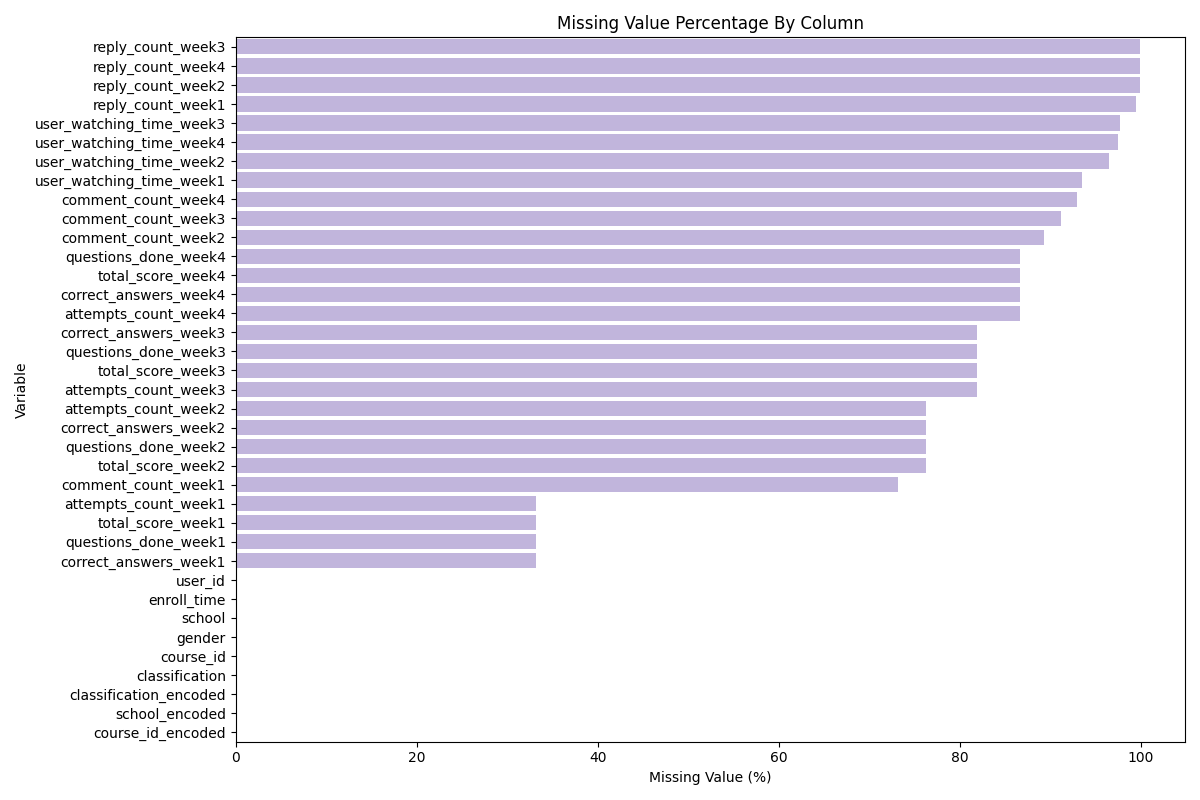
\includegraphics[width=0.9\textwidth]{imgs/missing-values-chart.png}
    \caption{Đặc điểm phân bố của dữ liệu thiếu trên các thuộc tính}
    \label{fig:percentage of missing values}
\end{figure}


 Trong \textbf{Hình \ref{fig:percentage of missing values}}, chúng ta có thể thấy được tình trạng đầy đủ của các trường dữ liệu. Đặc biệt, các thuộc tính liên quan đến hành vi học tập theo từng tuần như: \textit{reply\_count\_week3}, \textit{comment\_count\_week3}, \textit{attempts\_count\_week3} hay \textit{correct\_answer\_week3} đều có mức độ khuyết dữ liệu nghiêm trọng. Ngược lại, các cột định danh như \textit{user\_id}, \textit{course\_id}, cùng với một số thông tin đăng ký như \textit{enroll\_time}, lại có tỷ lệ thiếu không đáng kể hoặc gần như đầy đủ.

Tình trạng này gây ra trở ngại cho việc xây dựng mô hình dự đoán đáng kể do tính chất dữ liệu thiếu và không đồng nhất.


% \textbf{Hình \ref{fig:Histogram of Classification}} là biểu đồ tần suất của biến classification cho thấy sự phân bố không đồng đều giữa các nhóm xếp loại học tập. Trong đó, nhóm E chiếm tỷ lệ lớn nhất, vượt xa so với các nhóm còn lại với hơn 14.000 mẫu. Nhóm A xếp thứ hai với khoảng 6.000 mẫu, trong khi các nhóm B, C và D có số lượng tương đối thấp và khá cân bằng, dao động từ 1.000 đến 2.000 mẫu.

% Sự chênh lệch này phản ánh tính mất cân bằng nhãn (label imbalance) rõ rệt trong tập dữ liệu, đây là một yếu tố quan trọng cần được xem xét trong quá trình huấn luyện mô hình. Việc mất cân bằng có thể khiến mô hình nghiêng về việc dự đoán các lớp chiếm ưu thế như E và A, từ đó làm giảm độ chính xác đối với các lớp hiếm. Do đó, trong các bước tiếp theo, cần cân nhắc sử dụng các kỹ thuật xử lý mất cân bằng dữ liệu như oversampling, undersampling hoặc gán trọng số lớp để đảm bảo mô hình học được đầy đủ từ mọi phân lớp.

\begin{figure}[H]
    \centering
    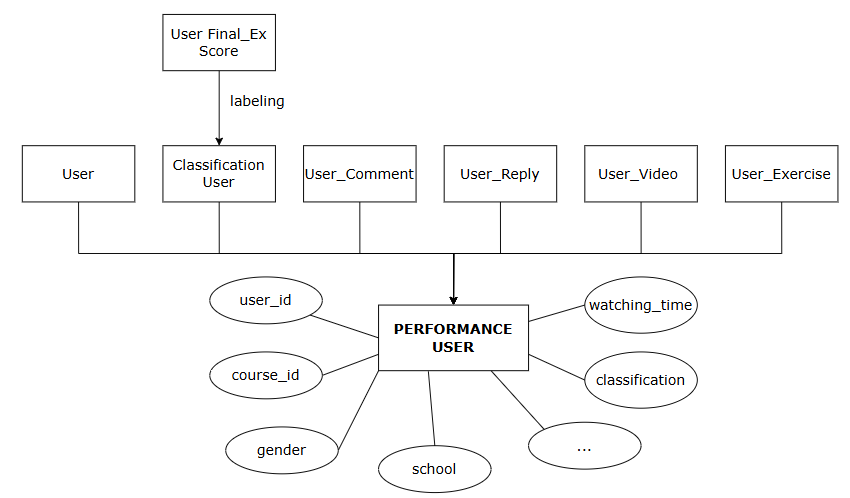
\includegraphics[width=0.9\textwidth]{imgs/data-transform.png}
    \caption{Quy trình chuyển đổi dữ liệu}
    \label{fig:data-transform}
\end{figure}

Sơ đồ tổng quan về quy trình chuyển đổi được minh họa trong Hình~\ref{fig:data-transform} cho chúng ta nắm bắt phương pháp chúng tôi hợp nhất các file dữ liệu.
Quá trình này bắt đầu từ thực thể \textbf{User}, đại diện cho người học trong nền tảng MOOC. Dữ liệu từ người dùng được liên kết với các nguồn dữ liệu phụ như:

\begin{itemize}
    \item \textbf{Classification User}: thông tin xếp loại người học dựa trên điểm số cuối kỳ.
    \item \textbf{User\_Comments} và \textbf{User\_Reply}: dữ liệu hành vi người dùng trên diễn đàn thảo luận (số lượng bình luận, trả lời).
    \item \textbf{User\_Video}: thông tin thời lượng người học xem video bài giảng.
    \item \textbf{User\_Exercise}: các tương tác của người dùng với bài tập (số lần nộp bài, số điểm đạt được, số câu đúng, \ldots).
\end{itemize}

Tất cả các nguồn dữ liệu phụ trên được liên kết trở lại với người học thông qua thực thể trung tâm \textbf{Performance User}, chứa các đặc trưng như:

\begin{itemize}
    \item \textbf{Thông tin cá nhân}: \textit{gender}, \textit{year\_of\_birth}, \textit{school}.
    \item \textbf{Thông tin hoạt động}: \textit{comment\_count}, \textit{reply\_count}, \textit{watching\_time}, \textit{assignment\_count}, \textit{final\_exam\_score}, \textit{v.v}.
\end{itemize}

Các tập dữ liệu rời rạc được liên kết với nhau thông qua các khóa định danh chính như \textit{user\_id} và \textit{course\_id}. Việc tổ chức dữ liệu theo cấu trúc Performance User đóng vai trò trung tâm. Thông qua quá trình tích hợp và chuẩn hóa theo chiều dọc dựa trên các khóa chính, dữ liệu được gom lại sao cho mỗi dòng trong bảng tổng hợp cuối cùng đại diện cho một cá nhân cụ thể, với đầy đủ các đặc trưng cần thiết cho mô hình dự đoán. 

\subsection{Chiến lược gán nhãn và chuẩn hóa thang điểm}
Dữ liệu từ nền tảng MOOCCubeX bao gồm hàng trăm khóa học đến từ nhiều quốc gia và tổ chức giáo dục khác nhau, với mỗi đơn vị áp dụng một hệ thống thang điểm riêng biệt (chẳng hạn: thang 10, thang 20, thang 4.0 của Mỹ, thang 6 của Đức, v.v.). Sự đa dạng này tạo ra thách thức trong việc chuẩn hóa để phục vụ cho quá trình quá trình dự đoán. Do đó, chúng tôi đã thực hiện một khảo sát các thang điểm hiện hành trên thế giới, giúp quá trình gán nhãn trở nên chính xác và đáng tin cậy hơn.

\subsubsection{Khảo sát thang điểm quốc tế}
Tổng cộng, nhóm đã khảo sát 73 hệ thống thang điểm khác nhau về: 
\begin{itemize}
    \item Loại thang điểm sử dụng (thang điểm 10, 20, 4.0, 6, 100, \ldots)
    \item Số lượng khóa học áp dụng mỗi loại thang điểm
    \item Sự tồn tại hay không của mô tả phân loại kết quả học tập
    \item Phân loại học lực tương ứng với các mức độ như: Xuất sắc, Giỏi, Khá, Trung bình, Yếu và Kém.
\end{itemize}

Trong đó, tôi tập trung vào 13 thang điểm phổ biến có đủ thông tin phân loại, như:

\begin{itemize}
    \item Thang 10 điểm (159 khóa học): 
    \textit{Phổ biến tại Việt Nam}
    
    \item Thang 5 điểm (106 khóa):
    \textit{Áp dụng rộng rãi tại Nga}

    \item Thang 20 điểm (87 khóa):
    \textit{Thường dùng ở Pháp}

    \item Thang 6 điểm (77 khóa):
    \textit{Theo hệ thống giáo dục Đức}

    \item Thang 4.0 (65 khóa):
    \textit{Một số đại học quốc tế sử dụng}
\end{itemize}


\subsubsection{Chiến lược chuẩn hóa về 5 mức độ của Coursera}

Sau quá trình khảo cứu nhiều hệ thống phân loại học lực từ các quốc gia và nền tảng đào tạo trực tuyến khác nhau, chúng tôi quyết định chuẩn hóa toàn bộ dữ liệu điểm số về \textbf{thang 5 mức độ} được sử dụng bởi nền tảng \textit{Coursera}, một trong những hệ thống MOOC lớn và có sức ảnh hưởng toàn cầu.

Việc lựa chọn thang điểm này không chỉ dựa trên tính phổ biến, mà còn bởi nó có cấu trúc rõ ràng, dễ hiểu, với các mức đánh giá cụ thể từ ``Xuất sắc'' đến ``Chưa hoàn thành''. Điều này đặc biệt quan trọng trong bối cảnh dữ liệu MOOCCubeX sử dụng nhiều thang điểm khác nhau do sự khác biệt của mỗi quốc gia, ví dụ thang điểm 10, thang điểm 20, GPA 4.0 hoặc thang điểm 6 của Đức. Thang điểm của Coursera giúp tạo nên một chuẩn chung, cho phép quy đổi linh hoạt và \textbf{giảm thiểu sai lệch do sự không đồng nhất trong hệ thống đánh giá ban đầu}.

Hơn nữa, hệ thống phân loại này được thiết kế với sự cân bằng giữa tính chi tiết và tính tổng quát, vừa phản ánh được năng lực học tập thực tế của người học, vừa phù hợp để tích hợp vào các mô hình học máy, nơi cần các nhãn nhất quán và dễ diễn giải. Việc sử dụng thang điểm 5 mức từ Coursera cũng giúp nâng cao \textbf{tính khả chuyển của kết quả mô hình}, đồng thời hỗ trợ dễ dàng hơn cho các phân tích so sánh liên quốc gia hoặc giữa các tổ chức giáo dục khác nhau.



\vspace{0.5em}
\begin{table}[H]
\centering
\caption{Chiến lược chuẩn hóa điểm số về thang điểm Coursera}
\label{tab:coursera_grading}
\renewcommand{\arraystretch}{1.6} 
\begin{tabular}{|c|>{\centering\arraybackslash}p{7cm}|>{\centering\arraybackslash}p{2.5cm}|}
\hline
\textbf{Mức độ} & \textbf{Mô tả} & \textbf{Nhãn gán} \\
\hline
Distinction & 85–100\% -- Xuất sắc, thành tích vượt trội & A \\
\hline
Merit & 70–84\% -- Giỏi, kiến thức vững & B \\
\hline
Pass & 50–69\% -- Đạt yêu cầu tối thiểu & C \\
\hline
Fail & Dưới 50\% -- Không đạt yêu cầu & D \\
\hline
Incomplete & Không làm bài thi cuối kỳ hoặc bỏ dở & E \\
\hline
\end{tabular}
\end{table}
\vspace{0.5em}

Việc gán nhãn này được thực hiện cho từng học viên trong mỗi khóa học, dựa trên thang điểm cụ thể mà khóa học đó sử dụng. Các quy tắc chuyển đổi được tham khảo từ tài liệu chính thức của từng quốc gia hoặc nền tảng MOOC, và được mã hóa thành logic tự động trong pipeline xử lý dữ liệu của hệ thống.
\noindent Dựa trên nguyên tắc trên, tôi đã tiến hành chuyển đổi các hệ thống thang điểm hiện có thành nhãn đầu ra phục vụ cho mô hình học sâu. Bảng dưới đây trình bày một số ví dụ điển hình của các hệ thống thang điểm có chiến lược gán nhãn rõ ràng:

\begin{table}[H]
\centering
\caption{Tổng hợp các hệ thống thang điểm và chiến lược gán nhãn}
\begin{tabular}{|c|p{2.5cm}|p{2.8cm}|p{6cm}|}
\hline
\textbf{STT} & \textbf{Thang điểm} & \textbf{Phân loại gốc} & \textbf{Chiến lược gán nhãn (theo Coursera)} \\
\hline
1 & 10 (Việt Nam) & Xuất sắc: 9-10; Giỏi: 8-<9; Khá: 7-<8; Trung bình: 5-<7; Yếu: 4-<5; Kém: <4 & 
A: 9-10 \newline
B: 8-<9 \newline
B: 7-<8 \newline
C: 5-<7 \newline
D: <5 \newline
E: Không thi cuối kỳ \\
\hline
2 & 5 (Nga) & Excellent (5), Good (4), Satisfactory (3), Unsatisfactory (2) & 
A: 5 \newline
B: 4 \newline
C: 3 \newline
D: 2 \newline
E: Không thi cuối kỳ \\
\hline
3 & 20 (Pháp) & Xuất sắc: 18-20; Giỏi: 16-<18; Khá: 14-<16; Trung bình: 10-<14; Kém: <10 & 
A: 18-20 \newline
B: 16-<18 \newline
B: 14-<16 \newline
C: 10-<14 \newline
D: <10 \newline
E: Không thi cuối kỳ \\
\hline
4 & 6 (Đức) & 1 (Very Good) đến 6 (Inadequate) & 
A: 1 \newline
B: 2 \newline
C: 3-4 \newline
D: 5-6 \newline
E: Không thi cuối kỳ \\
\hline
5 & 100 (Mỹ) & Xuất sắc: 90-100; Giỏi: 80-89; Khá: 70-79; Trung bình khá: 60-69; Trung bình: 50-59; Kém: <50 & 
A: 90-100 \newline
B: 80-89 \newline
B: 70-79 \newline
C: 50-69 \newline
D: <50 \newline
E: Không thi cuối kỳ \\
\hline
\end{tabular}
\label{tab:grading_conversion}
\end{table}

Kết quả cho thấy việc quy đổi điểm số về thang 5 mức không chỉ tạo ra một thuộc tính chung, mà còn giúp cải thiện hiệu quả huấn luyện.

 
% Để xây dựng hệ thống khuyến nghị khóa học, khoá luận đã thực hiện các thí nghiệm sử dụng dữ liệu từ bộ dữ liệu MOOCCubeX của nền tảng MOOC XuetangX tại Trung Quốc. Bộ dữ liệu này bao gồm thông tin về người dùng, các khóa học họ đã đăng ký, và các danh mục khóa học tương ứng (tham khảo Bảng \ref{tab:right} để biết thêm chi tiết).
% Với dữ liệu khoá học được mô tả trong bảng \ref{tab:course_info}, em em có các thuộc tính như sau:
Sau đó, chúng tôi tiến hành tiền xử lý bằng cách lọc và tổng hợp các hành vi học tập của người dùng trong bốn tuần đầu kể từ thời điểm ghi danh, đây là giai đoạn được xem là có ảnh hưởng lớn đến khả năng hoàn thành khóa học.
Bộ dữ liệu sau xử lý bao gồm 16.267 người học, được phân bố trên 174 khóa học khác nhau từ nhiều lĩnh vực và thuộc về 915 trường học hoặc tổ chức giáo dục. Dựa trên chiến lược gán nhãn và chuẩn hóa thang điểm đã đề cập, kết quả hoàn thành khóa học cuối cùng của người học được chia thành năm nhóm theo mức độ hoàn thành chuẩn đầu ra, bao gồm: A (Xuất sắc), B (Tốt), C (Đạt yêu cầu), D (Chưa đạt) và E (Không hoàn thành khóa học).
\begin{figure}[H]
    \centering
    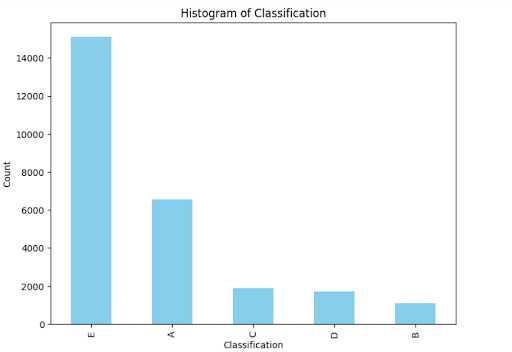
\includegraphics[width=0.9\textwidth]{imgs/Histogram of Classification.png}
    \caption{Biểu đồ phân phối nhãn học lực sau chuẩn hóa}
    \label{fig:label}
\end{figure}

Hình  \ref{fig:label} phản ánh sự mất cân bằng dữ liệu: nhóm E (Không hoàn thành) chiếm phần lớn với 61,14\%, theo sau là nhóm A (Xuất sắc) với 22,88\%. Trong khi đó, các nhóm còn lại lần lượt là B (3,37\%), C (6,34\%), và D (6,27\%), là các nhóm thể hiện hiệu suất trung bình hoặc yếu nhưng chiếm tỷ lệ thấp hơn nhiều. 
\begin{table*}[htbp]
\caption{Tổng quan bộ dữ liệu và phân bố nhãn}
\label{tab:combined-tables}
\centering
\begin{minipage}[t]{0.65\textwidth} % mở rộng bảng mô tả
\centering
\small % giảm cỡ chữ bảng mô tả
\renewcommand{\arraystretch}{1.3}
\textbf{(a) Mô tả bộ dữ liệu}
\vspace{2mm}

\begin{tabularx}{\textwidth}{|>{\raggedright\arraybackslash}p{3.4cm}|>{\centering\arraybackslash}m{1.2cm}|>{\raggedright\arraybackslash}X|}
\hline
\textbf{Đặc trưng} & \textbf{Loại dữ liệu} & \textbf{Mô tả} \\
\hline
User & Object & Người dùng đã đăng ký khóa học \\
Course & Object & Khóa học mà người học đăng ký \\
School & Object & Trường mà người học theo học \\
Gender & Integer & Giới tính của người học \\
Enroll\_time & Datetime & Thời điểm đăng ký khóa học \\
comment\_count\_week \textit{i} & Float & Số lượng bình luận trong tuần \textit{i} \\
reply\_count\_week \textit{i} & Float & Số lượng phản hồi trong tuần \textit{i} \\
questions\_done\_week \textit{i} & Float & Số lượng câu hỏi đã làm trong tuần \textit{i} \\
attempts\_count\_week \textit{i} & Float & Số lần làm bài kiểm tra trong tuần \textit{i} \\
correct\_answers\_week \textit{i} & Float & Số lượng câu trả lời đúng trong tuần \textit{i} \\
total\_score\_week \textit{i} & Float & Tổng điểm bài kiểm tra trong tuần \textit{i} \\
user\_watching\_time\_week \textit{i} & Float & Tổng thời lượng xem video (giờ) trong tuần \textit{i} \\
classification & Object & Nhãn kết quả hoàn thành khóa học cuối cùng \\
\hline
\multicolumn{3}{l}{$^{\mathrm{*}}$\textit{i} đại diện cho tuần 1 - 4.}
\end{tabularx}
\end{minipage}
\hfill
\begin{minipage}[t]{0.32\textwidth} % thu hẹp bảng phân phối
\centering
\small % giảm cỡ chữ bảng label
\renewcommand{\arraystretch}{1.3}
\textbf{(b) Tỷ lệ phân bố nhãn}
\vspace{2mm}

\begin{tabular}{|c|c|c|}
\hline
\textbf{Nhãn} & \textbf{Số lượng} & \textbf{Tỷ lệ} \\
\hline
A  & 3,722 & 22.88\% \\
B  & 548 & 3.37\% \\
C  & 1,032 & 6.34\% \\
D  & 1,020 & 6.27\% \\
E  & 9,945 & 61.14\% \\
\hline
\textbf{Tổng} & 16,267 & 100.00\% \\
\hline
\end{tabular}
\end{minipage}
\end{table*}
Sự chênh lệch đáng kể này tạo ra một bài toán mất cân bằng lớp (class imbalance), khi mô hình học máy thường có xu hướng thiên lệch về các lớp có tần suất xuất hiện cao hơn, dẫn đến tình trang học hỏi kém hiệu quả với những lớp nhãn ít xuất hiện.

Đây chính là vấn đề chúng ta thường gặp khi giải quyết các bài toán phân loại. Nhằm bảo vệ dữ liệu có tần suất xuất hiện thấp (như nhóm D (không đạt)), chúng ta có những phương pháp tăng mẫu dữ liệu, điển hình là phương pháp tổng hợp mẫu thiểu số SMOTE. Mục tiêu chính là nâng cao khả năng nhận biết của mô hình đối với các nhóm dữ liệu thiểu số.
% ------
\section{Phương pháp đề xuất}
Mục tiêu của phần này là làm rõ cách mô hình hoạt động và quy trình GCN-I thực hiện suy diễn giá trị thiếu, tất cả nhằm hướng đến việc cải thiện chất lượng của bộ dữ liệu đầu vào.

\begin{figure}[t]
    \centering
    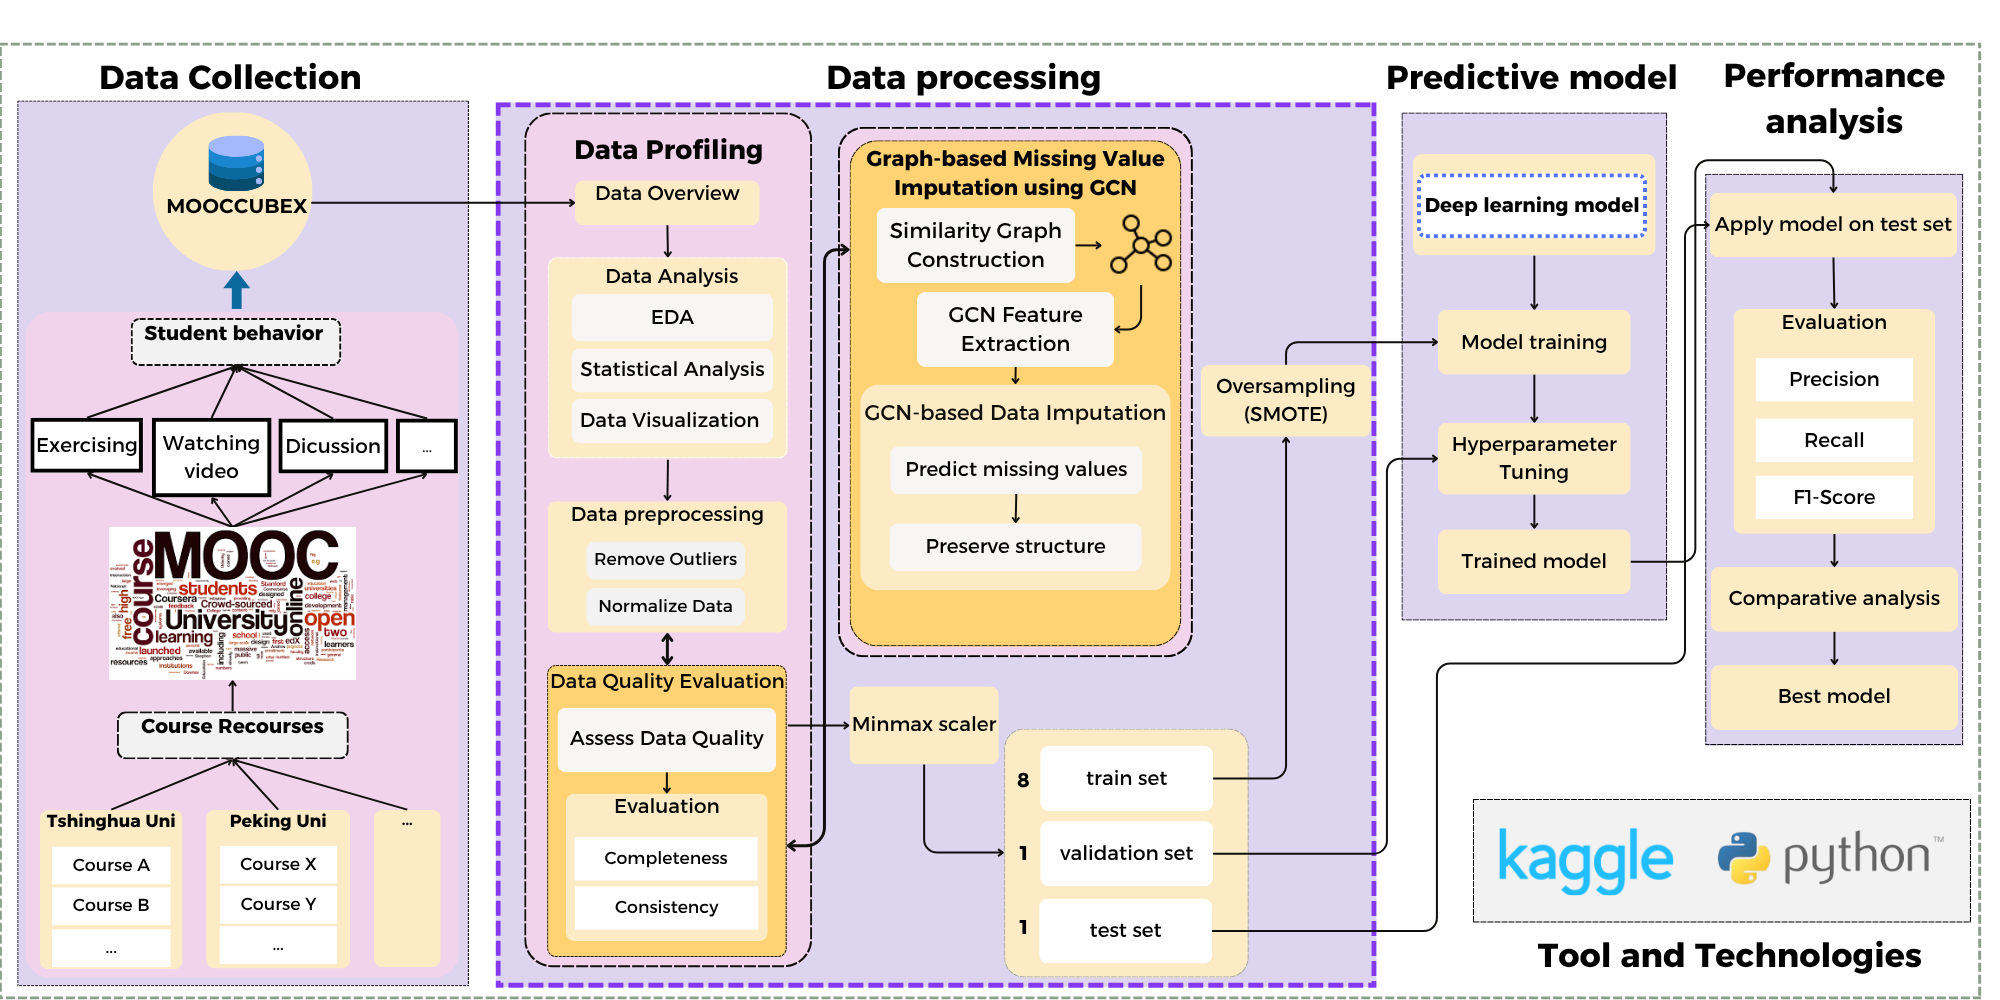
\includegraphics[width = \textwidth]{imgs/system-logo.png}
    \caption{Flowchart thể hiện quy trình hệ thống}
    \label{fig:System-img}
\end{figure}
  Quy trình xử lý dữ liệu tổng thể của nghiên cứu được thể hiện qua sơ đồ ở \textbf{Hình \ref{fig:System-img}}. Toàn bộ kiến trúc được cấu thành từ bốn bước chính: thu thập dữ liệu, tiền xử lý, huấn luyện mô hình và phân tích kết quả. 

Đầu tiên là thu thập dữ liệu từ các nền tảng MOOCs, gồm thông tin về sinh viên cùng với thông tin khóa học. Sau bước thu thập, dữ liệu được đưa vào quy trình tiền xử lý  bao gồm bốn bước chính: Data Overview, Data Analysis, Data Preprocessing và Data Quality Evaluation. Tổng thể của dữ liệu được nắm bắt thông qua các kiểm tra kích thước, loại thuộc tính và tỷ lệ thiếu giá trị. Chúng tôi thể hiện các xu hướng phân phối dữ liệu hoặc mối quan hệ giữa các biến bằng biểu đồ trực quan hóa và thống kê mô tả. Tiếp theo, việc đánh giá chất lượng dữ liệu được thực hiện để xác định tình trạng hiện tại của dữ liệu, từ đó đưa ra các quyết định điều chỉnh phù hợp. Những điểm dữ liệu cực đoan có khả năng gây nhiễu quá trình huấn luyện, thông qua phương pháp khoảng tứ phân vị (IQR) kết hợp với biểu đồ hộp (Box Plot), chúng ta tiến hành loại bỏ. 

Khác với các quy trình truyền thống chỉ thực hiện một vòng xử lý, chúng tôi tiến hành đánh giá chất lượng dữ liệu nhiều lần, đặc biệt là sau khi hoàn tất các bước xử lý sơ bộ. Mục tiêu là kiểm tra mức độ cải thiện đạt được, từ đó đảm bảo tập dữ liệu đã sẵn sàng cho giai đoạn suy diễn giá trị thiếu bằng phương pháp GCN mà nghiên cứu đề xuất.


GCN-I được chúng tôi áp dụng để suy diễn giá trị khuyết của tập dữ liệu, trong đó các nút biểu diễn người học và các cạnh đại diện cho các thuộc tính chung như trường học, khóa học đã đăng ký hoặc sự tương đồng dữ liệu. Nếu mật độ cạnh quá thấp, chúng tôi sẽ thêm các cạnh bổ sung dựa trên các chỉ số tương đồng. Cơ chế bổ sung giá trị được xây dựng trên kiến trúc hai giai đoạn Generator–Discriminator như \textbf{Hình \ref{fig:GCN-Imputer}}. Khác với GCN truyền thống, kiến trúc này nâng cao độ chính xác khi bổ sung giá trị thiếu thông qua học đối kháng, cho phép bộ sinh (generator) liên tục cải thiện các giá trị khuyết dựa trên phản hồi từ bộ phân biệt (discriminator). Chúng tôi áp dụng chỉ số sai số bình phương trung bình (MSE) giữa các giá trị thực và giá trị được bổ sung để đánh giá chất lượng của quá trình điền khuyết. Sau khi hoàn thành quá trình, quá trình đánh giá chất lượng được thực hiện lại theo các độ đo chất lượng trực tiếp và gián tiếp, giúp theo dõi chặt chẽ sự cải thiện và đảm bảo dữ liệu đầu vào sạch, tối ưu cho các bước học máy tiếp theo.

Sau khi hoàn tất quá trình bổ sung giá trị thiếu bằng phương pháp GCN, dữ liệu được tiếp tục xử lý bằng  MinMax Scaler nhằm đưa các đặc trưng về cùng một khoảng giá trị chuẩn. Tập dữ liệu sau đó được phân chia thành ba phần theo tỷ lệ 8:1:1, tương ứng với các tập Train, Validation và Test.

Một trong những thách thức ban đầu được ghi nhận là tình trạng mất cân bằng lớp (class imbalance) trong tập dữ liệu. Để giải quyết vấn đề này và đảm bảo mô hình không bị thiên vị về phía các lớp đa số, chúng tôi đã áp dụng kỹ thuật lấy mẫu vượt trội cho lớp thiểu số tổng hợp, hay còn gọi là SMOTE (Synthetic Minority Over-sampling Technique). Kỹ thuật này giúp cân bằng lại sự phân bố của các nhãn, qua đó tăng cường khả năng nhận diện của mô hình đối với các nhóm thiểu số.

Khi chuẩn bị xong dữ liệu, quá trình huấn luyện mô hình học sâu được bắt đầu, bao gồm: 4-layer Stacked LSTM, GRU, RNN và BiLSTM. Để có một sự so sánh khách quan và toàn diện, hiệu năng của mỗi mô hình được định lượng thông qua một bộ các chỉ số đánh giá đa dạng. Mô hình thể hiện hiệu suất tốt nhất qua các bài kiểm tra này sẽ được lựa chọn để tích hợp làm nhân xử lý chính cho hệ thống website dự đoán kết quả hoàn thành khóa học.
\subsubsection{Kiến trúc GCN-Imputer}

\begin{figure}[t]
    \centering
    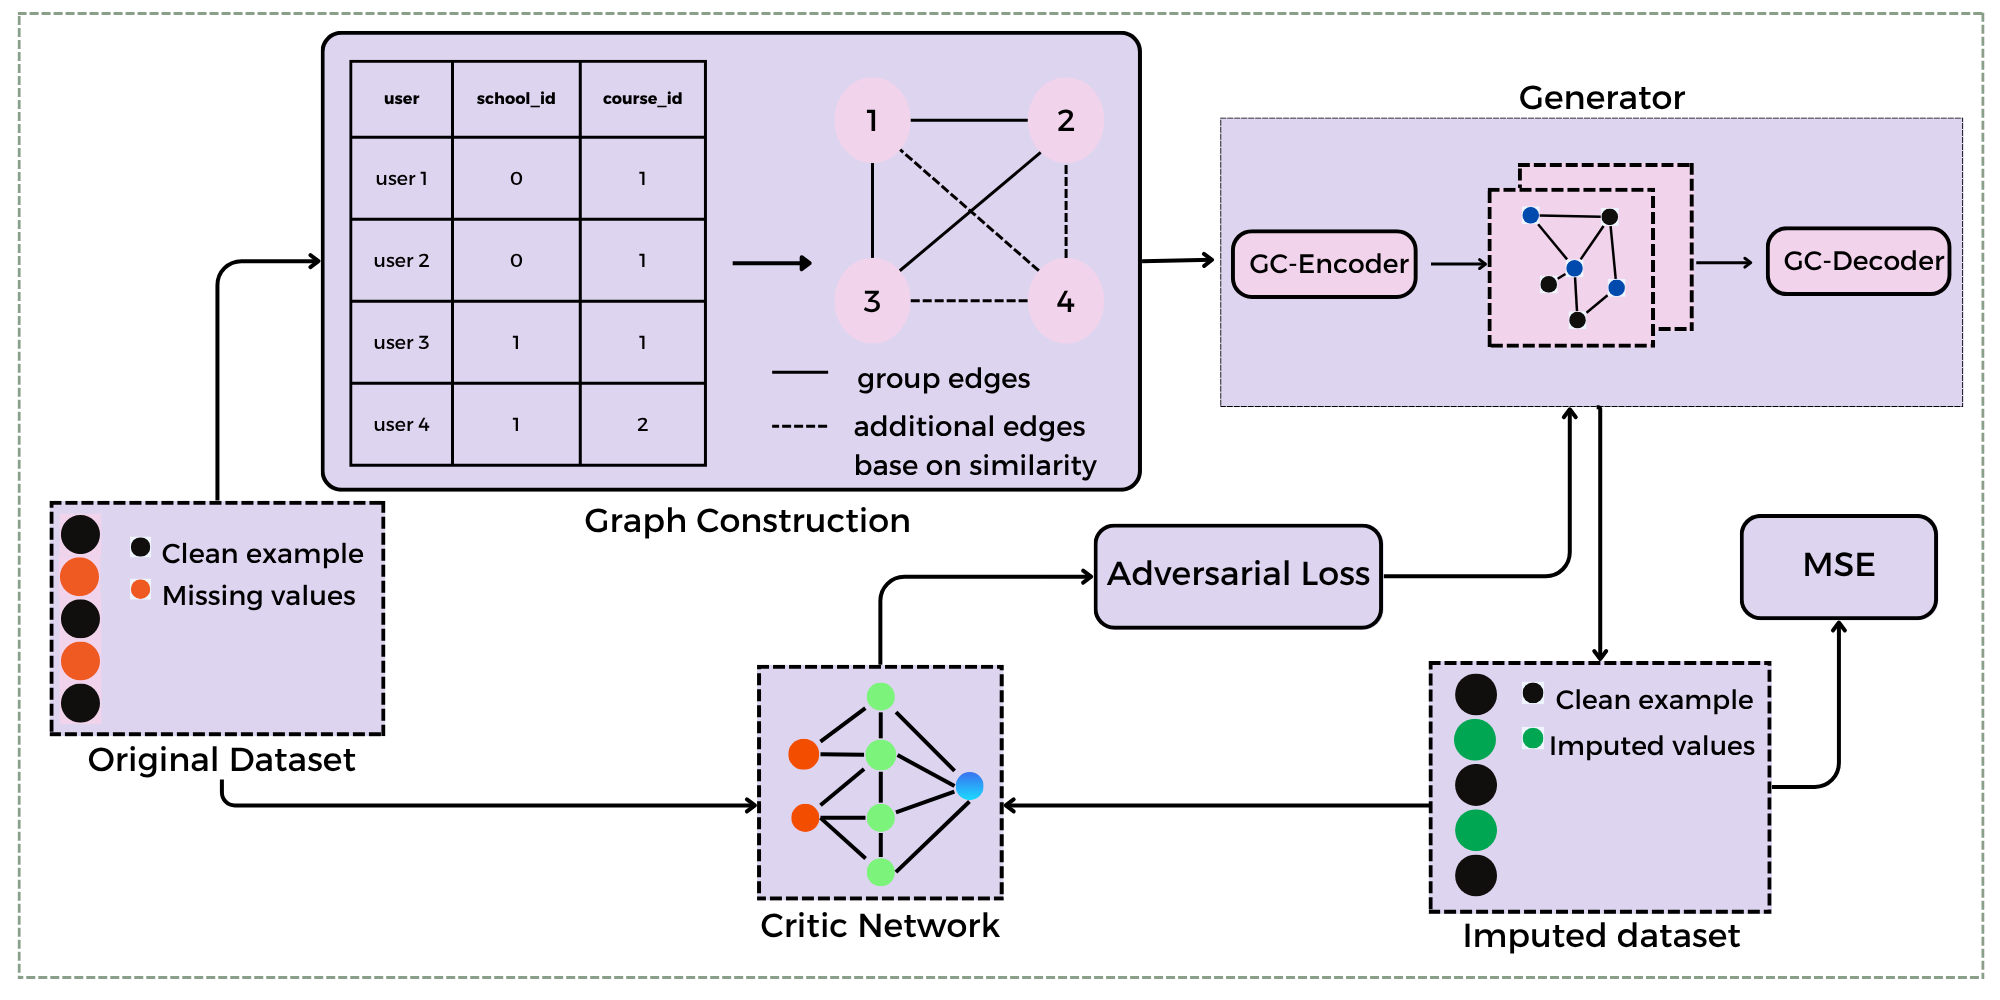
\includegraphics[width = \textwidth]{imgs/gcn-newtone.png}
    \caption{Kiến trúc mô hình GCN-Imputer}
    \label{fig:GCN-Imputer}
\end{figure}
Mô hình GCN-Imputer được thể hiện ở (\textbf{Hình \ref{fig:GCN-Imputer}}), một phương pháp hoàn thiện dữ liệu dựa trên GCN, kết hợp với mô hình sinh–phân biệt (Generator–Discriminator). Kiến trúc này không chỉ tận dụng được thông tin cấu trúc từ dữ liệu gốc thông qua xây dựng đồ thị, mà còn nâng cao độ chính xác của giá trị được điền bằng cách học sinh dữ liệu và phân biệt theo hướng đối kháng (adversarial learning). 

\textbf{Biểu diễn dữ liệu dưới dạng đồ thị (Graph Construction):} Thay vì xử lý dữ liệu theo dạng bảng truyền thống, phương pháp này bắt đầu bằng việc chuyển đổi dữ liệu ban đầu thành một ma trận đặc trưng, và xây dựng các thể (người học) là các đỉnh của đồ thị. Chúng tôi xác định sự tương đồng về đặc trưng hoặc mối quan hệ nhóm để xây dựng các liên kết (cạnh). Bằng cách biểu diễn dữ liệu như vậy, các thông tin về cấu trúc và những liên kết tiềm ẩn giữa các bản ghi có thể được làm rõ.

\vspace{0.5em}

\textbf{Bộ sinh (Generator):} Generator bao gồm một encoder và một decoder sử dụng GCN. Bộ encoder học biểu diễn đặc trưng dữ liệu có khuyết thiếu, trong khi decoder sử dụng các đặc trưng đó để ước lượng và điền vào các giá trị còn thiếu. Đây là bước học sinh tích cực nhằm tái tạo dữ liệu đầy đủ.

\vspace{0.5em}

\textbf{Bộ phân biệt (Critic/Discriminator):} Bộ Critic đóng vai trò như một mạng nơ-ron phân biệt, đánh giá xem các giá trị trong tập dữ liệu đầu ra là thật (clean) hay được điền vào (imputed). Trong quá trình huấn luyện, Critic và Generator được tối ưu theo hướng đối kháng, tương tự như trong GANs. Điều này tạo ra động lực để Generator sinh ra các giá trị khuyết một cách tự nhiên và sát với phân phối dữ liệu thật nhất.

\vspace{0.5em}

\textbf{Hàm mất mát (Loss Function):} Kiến trúc sử dụng kết hợp \textit{adversarial loss} và \textit{mean squared error (MSE)} để cân bằng giữa khả năng tái tạo chính xác và sự chân thực của dữ liệu được điền vào.

Kiến trúc GCN-Imputer nổi bật nhờ cơ chế học đối kháng giữa hai thành phần chính: Generator và Discriminator (Critic Network). Sự đối kháng này đóng vai trò như một quá trình huấn luyện hai mạng nơ-ron theo kiểu "thi đấu" – trong đó Generator cố gắng tạo ra các giá trị bị thiếu sao cho chúng không thể bị phân biệt với dữ liệu gốc, còn Critic học cách phát hiện các giá trị được điền vào. Cơ chế này thúc đẩy Generator tạo ra các giá trị suy đoán có tính xác thực cao và phân phối gần giống với dữ liệu gốc. Nhờ đó, các giá trị được bổ sung trở nên tự nhiên và phù hợp hơn với đặc điểm thống kê của tập dữ liệu ban đầu. Bên cạnh đó, sự kết hợp giữa hàm mất mát truyền thống như MSE và thành phần adversarial loss cho phép mô hình khai thác hiệu quả cả khía cạnh định lượng và định tính trong quá trình học. Chính sự tích hợp giữa phương pháp học biểu diễn dựa trên đồ thị và cơ chế học đối kháng đã đóng vai trò then chốt trong việc nâng cao hiệu quả của quá trình bổ sung dữ liệu, tạo nên bước tiến đáng kể mà GCN-Imputer đạt được.
\chapter{Thực nghiệm và đánh giá}
\label{chap:chap5}
\section{Đánh giá chất lượng dữ liệu}

Để đảm bảo và theo dõi chất lượng của bộ dữ liệu trong suốt vòng đời nghiên cứu, chúng tôi đã thiết lập một quy trình đánh giá định kỳ. Quy trình này được thực hiện tại hai thời điểm then chốt: trước và sau giai đoạn tiền xử lý dữ liệu. Khung đánh giá của chúng tôi tập trung vào bốn khía cạnh cốt lõi, được đo lường thông qua các chỉ số trực tiếp và gián tiếp. Các chỉ số này bao gồm: \textbf{tính đầy đủ} (completeness), \textbf{tính nhất quán} (consistency), \textbf{mức độ liên quan} (relevance) và \textbf{độ tin cậy} (reliability). 

\textbf{Completeness}\cite{nguyen2025data} thể hiện mức độ mà các thông tin cần thiết đã được ghi nhận đầy đủ trong tập dữ liệu, không bị khuyết thiếu. Một tập dữ liệu được xem là đạt tiêu chuẩn về tính đầy đủ khi các thuộc tính chứa giá trị hợp lệ ở mỗi bản ghi. Cách đo như sau: 

\begin{equation}
\text{Completeness}_{object} = \frac{|\{ a_i \in A \mid a_i \neq \text{NaN} \land a_i \neq \text{None} \}|}{|A|} \times 100
\end{equation}
\begin{equation}
\text{Completeness}_{dataset} = \frac{1}{N} \sum_{j=1}^{N} \text{Completeness}_{object_j}
\end{equation}
Trong đó, $A = \{a_1, a_2, \ldots, a_n\}$ là tập các thuộc tính của một đối tượng, $a_i$ là giá trị của thuộc tính thứ $i$, $|A|$ là tổng số thuộc tính, và tử số là số lượng thuộc tính có giá trị không bị thiếu.

Chỉ số này giúp xác định tỷ lệ dữ liệu có sẵn so với tổng số giá trị kỳ vọng. Việc đảm bảo tính đầy đủ là mục tiêu quan trọng trong giai đoạn tiền xử lý dữ liệu.


\textbf{Consistency} \cite{nguyen2025data} đánh giá mức độ mà các giá trị trong tập dữ liệu tuân thủ các quy tắc hoặc ràng buộc logic đã được định nghĩa trước. Đây là một tiêu chí quan trọng để đảm bảo rằng dữ liệu không chứa các sai sót mang tính logic hoặc mâu thuẫn nội tại giữa các trường thông tin. Cách đo như sau:

\begin{equation}
\text{Consistency}_{object} = \frac{|\{ c_j \in C \mid isValid(c_j) = \text{True} \}|}{|C|}
\end{equation}

\begin{equation}
\text{Consistency}_{dataset} = \frac{1}{N} \sum_{j=1}^{N} \text{Consistency}_{object_j}
\end{equation}

Trong đó, $C = \{c_1, c_2, \ldots, c_m\}$ là tập các điều kiện kiểm tra áp dụng cho một đối tượng, $isValid(c_j)$ là hàm đánh giá xem điều kiện $c_j$ có được thỏa mãn hay không, và $|C|$ là tổng số điều kiện kiểm tra.

Tính nhất quán của tập dữ liệu được đánh giá dựa trên một loạt điều kiện kiểm tra được định nghĩa trước, phản ánh các quy tắc về cấu trúc và ngữ nghĩa, bao gồm:

\begin{itemize}
    \item \textbf{Ràng buộc miền giá trị (Domain range):} $a_i \in [v_{\text{min}}, v_{\text{max}}]$
    \item \textbf{Không rỗng (Non-null):} $a_i \neq \text{null}$
    \item \textbf{Kiểu dữ liệu (Data type):} $a_i \in \text{type}(a_i)$
    \item \textbf{Ràng buộc logic (Logical constraints):} ví dụ $a_i > a_j$
    \item \textbf{Tính duy nhất (Uniqueness):} $a_i \notin \text{duplicates}(A)$
    \item \textbf{Toàn vẹn khóa ngoại (Foreign key integrity):} $a_i \in \text{ReferenceTable}$
\end{itemize}

Các quy tắc kiểm tra này đóng vai trò nền tảng để tính toán chỉ số nhất quán và hỗ trợ phát hiện các vi phạm ngữ nghĩa trong tập dữ liệu. \textbf{Các nhóm trường dữ liệu được kiểm tra và quy tắc áp dụng:}

\begin{itemize}
    \item[(a)] \textbf{Các trường định danh và phân loại:}
    \begin{itemize}
        \item \texttt{user\_id}, \texttt{course\_id}, \texttt{school}: không được thiếu (\texttt{null}) và phải đúng kiểu \texttt{object}.
        \item \texttt{gender}: chỉ nhận các giá trị \{0, 1, 2\} hoặc để trống.
        \item \texttt{enroll\_time}: phải có định dạng ngày giờ hợp lệ.
        \item \texttt{classification}: chỉ chấp nhận các giá trị thuộc tập \{A, B, C, D, E\}.
    \end{itemize}

    \item[(b)] \textbf{Các trường hành vi theo tuần (Tuần 1–4):}
    \begin{itemize}
        \item \texttt{comment\_count\_week\{n\}}, \texttt{reply\_count\_week\{n\}}: là số nguyên không âm.
        \item \texttt{questions\_done\_week\{n\}}: $\geq 0$.
        \item \texttt{attempts\_count\_week\{n\}}: $\geq$ \texttt{questions\_done\_week\{n\}}.
        \item \texttt{correct\_answers\_week\{n\}}: $\leq$ \texttt{questions\_done\_week\{n\}}.
        \item \texttt{total\_score\_week\{n\}}: $\geq 0$.
        \item \texttt{user\_watching\_time\_week\{n\}}: $\geq 0$.
    \end{itemize}

    \item[(c)] \textbf{Kiểm tra toàn bộ bản ghi:}
    \begin{itemize}
        \item Kiểm tra tính \textit{duy nhất} của từng bản ghi bằng cách phát hiện các dòng trùng lặp hoàn toàn.
    \end{itemize}
\end{itemize}

\textbf{Kết quả đầu ra:} Sau khi kiểm tra, hệ thống trả về:
\begin{itemize}
    \item Tỷ lệ bản ghi hoàn toàn hợp lệ (\textit{record-level consistency}).
    \item Tỷ lệ ô dữ liệu hợp lệ (\textit{cell-level consistency}).
    \item Tỷ lệ trung bình theo trường dữ liệu (\textit{object-level consistency}).
    \item Danh sách các quy tắc bị vi phạm nhiều nhất để phục vụ phân tích nguyên nhân.
\end{itemize}

Kiểm tra tính nhất quán cho phép nhận diện các sai lệch trong hành vi học tập, lỗi về định dạng hoặc các mâu thuẫn giữa các trường dữ liệu. 

\textbf{Reliability (Độ tin cậy):} Chỉ số này đo lường sự ổn định và nhất quán của các kết quả dự đoán mà một mô hình học máy có thể tạo ra từ một bộ dữ liệu nhất định. Trong lĩnh vực phân tích dữ liệu học tập, độ tin cậy thể hiện liệu rằng bộ dữ liệu đầu vào có đủ tốt để các mô hình khác nhau, hoặc cùng một mô hình qua các lần huấn luyện khác nhau, đều đưa ra những kết luận dự báo tương tự nhau hay không. Vì đây là một thuộc tính gián tiếp, không thể đo lường trực tiếp như các thuộc tính cấu trúc (độ đầy đủ, độ nhất quán), chúng tôi đánh giá nó thông qua hiệu năng dự đoán của mô hình. Cụ thể, hai chỉ số phổ biến là F1-score và Accuracy được sử dụng làm thước đo đại diện\cite{zhang2019reliability}.  


\textbf{Relevance}: Mức độ liên quan phản ánh khả năng của các thuộc tính trong tập dữ liệu đóng góp vào việc giải thích hoặc dự đoán biến mục tiêu. Một thuộc tính được xem là có tính liên quan cao nếu nó mang lại thông tin hữu ích cho mô hình, giúp mô hình phân biệt rõ ràng giữa các lớp nhãn.

Khác với các tiêu chí như tính đầy đủ (Completeness) hay tính nhất quán (Consistency), mức độ liên quan (Relevance) mang tính trừu tượng và không thể đánh giá trực tiếp từ dữ liệu thô. Vì vậy, trong nghiên cứu này, chúng tôi sử dụng phương pháp gián tiếp để đo lường Relevance, thông qua chỉ số AUC-ROC (Area Under the Receiver Operating Characteristic Curve), nhằm phản ánh khả năng phân biệt giữa các nhãn đầu ra của mô hình trên cơ sở dữ liệu đã xử lý.
\begin{itemize}
    \item \textbf{AUC-ROC:} Là chỉ số đo diện tích dưới đường cong ROC, biểu thị mức độ mà mô hình có thể phân biệt chính xác giữa các lớp. Giá trị AUC càng lớn cho thấy dữ liệu đầu vào càng giàu thông tin và được tính toán theo công thức:

    \begin{equation}
        \text{AUC} = \int_{0}^{1} TPR(FPR^{-1}(x)) \, dx
    \end{equation}

    Trong đó:
    \begin{itemize}
        \item \textbf{TPR (True Positive Rate)} = $\frac{TP}{TP + FN}$
        \item \textbf{FPR (False Positive Rate)} = $\frac{FP}{FP + TN}$
    \end{itemize}
\end{itemize}

Dữ liệu có mức độ liên quan (Relevance) cao thường cho phép mô hình đạt AUC-ROC gần 1.0, cho thấy khả năng phân biệt giữa các lớp rất tốt. Ngược lại, nếu dữ liệu thiếu thông tin quan trọng hoặc nhiễu, AUC sẽ tiệm cận 0.5, tương đương với việc mô hình dự đoán ngẫu nhiên. Vì vậy, việc nâng cao độ liên quan thông qua các kỹ thuật như chọn lọc đặc trưng (feature selection), xây dựng đặc trưng mới (feature engineering), hoặc tích hợp thêm dữ liệu có giá trị là điều thiết yếu. 

\section{Tiêu chí đánh giá hiệu suất mô hình}
 Nhằm phản ánh chính xác mức độ cân bằng giữa các lớp và mang lại góc nhìn đánh giá khách quan và toàn diện hơn, ngoài các độ đo cơ bản như \textbf{Precision}, \textbf{Recall} và \textbf{F1-Score}, nghiên cứu này còn kết hợp sử dụng hai phương pháp tính trung bình: \textbf{macro average} và \textbf{weighted average}.

\begin{itemize}
    \item \textbf{Macro Average:} Tính trung bình F1-score trên tất cả các lớp, mà không quan tâm đến kích thước (số lượng mẫu) của từng lớp. Điều này đảm bảo rằng các lớp hiếm không bị “lấn át” bởi các lớp phổ biến.
    \begin{equation}
        \text{F1}_{\text{macro}} = \frac{1}{N} \sum_{i=1}^{N} \text{F1}_i
    \end{equation}
    Trong đó $N$ là số lớp, và $\text{F1}_i$ là F1-score của lớp thứ $i$.

    \item \textbf{Weighted Average:} Tính trung bình F1-score theo trọng số của từng lớp, với trọng số là tỷ lệ xuất hiện của lớp đó trong tập dữ liệu. Cách tính này phản ánh chính xác hơn hiệu suất mô hình trong toàn bộ tập mẫu.
    \begin{equation}
        \text{F1}_{\text{weighted}} = \sum_{i=1}^{N} w_i \times \text{F1}_i
    \end{equation}
    Với $w_i = \frac{n_i}{\sum_j n_j}$ là tỷ lệ mẫu thuộc lớp $i$ trên toàn bộ tập dữ liệu.
\end{itemize}

\textbf{Ý nghĩa:} 
\begin{itemize}
    \item F1-macro cho biết hiệu suất đồng đều của mô hình giữa các lớp.
    \item F1-weighted cho biết hiệu suất tổng thể có tính đến phân bố lớp.
\end{itemize}

\textbf{Ứng dụng:} Việc tính toán đồng thời F1-macro và F1-weighted cho mỗi mô hình học máy đảm bảo việc đánh giá hiệu suất là toàn diện và công bằng với tất cả các lớp. Các chỉ số này phản ánh khả năng mô hình mở rộng và thích ứng trong các tình huống thực tế. Điều này đặc biệt có ý nghĩa đối với các lớp dữ liệu thiểu số, chẳng hạn như nhóm người học có kết quả thấp.
\section{Phương pháp thực nghiệm}
\begin{table}[!htbp]
\centering
\caption{Preprocessing Strategies and Baseline Models}
\label{tab:baseline-models}
\scriptsize
\renewcommand{\arraystretch}{1.2}
\setlength{\tabcolsep}{1pt}
\resizebox{\columnwidth}{!}{%
\begin{tabular}{|c|c|c|c|c|c|c|c|c|c|c|c|}
    \hline
    \multirow{2}{*}{} & \multicolumn{7}{c|}{\textbf{Preprocessing}} & \multicolumn{4}{c|}{\textbf{Model}} \\ 
    \cline{2-12}
    & Raw & LD & Mean & Median & KNN & KI & GCN & LSTM & GRU & RNN & BiLSTM \\ 
    \hline
    Zero-1     & \checkmark &        &       &        &       &     &      & \checkmark & \checkmark & \checkmark & \checkmark \\ 
    \hline
    Drop-2     &            & \checkmark &   &        &       &     &      & \checkmark & \checkmark & \checkmark & \checkmark \\ 
    \hline
    Mean-3     &            &        & \checkmark &   &       &     &      & \checkmark & \checkmark & \checkmark & \checkmark \\ 
    \hline
    Median-4   &            &        &       & \checkmark &   &     &      & \checkmark & \checkmark & \checkmark & \checkmark \\ 
    \hline
    KNN-5      &            &        &       &        & \checkmark &  &      & \checkmark & \checkmark & \checkmark & \checkmark \\ 
    \hline
    KI-6       &            &        &       &        &        & \checkmark &  & \checkmark & \checkmark & \checkmark & \checkmark \\
    \hline
    \textbf{GCN-I} &        &        &       &        &       &     & \checkmark & \checkmark & \checkmark & \checkmark & \checkmark \\ 
    \hline
\end{tabular}
}
\vspace{0.5em}
\raggedright \scriptsize
\textit{Note: LD = Listwise Deletion.}
\end{table}
Để đánh giá một cách định lượng hiệu quả của phương pháp GCN-I, một phân tích so sánh đã được thực hiện. Phương pháp của chúng tôi được đối chiếu với năm kỹ thuật xử lý dữ liệu thiếu phổ biến, được xem như các mô hình cơ sở (baseline models). Tất cả các kỹ thuật này đều được áp dụng ở giai đoạn tiền xử lý, trước khi đưa dữ liệu vào huấn luyện các mô hình học sâu. Dưới đây là mô tả chi tiết về từng phương pháp cơ sở:

\begin{itemize}
    \item \textbf{Zero-1 (Điền khuyết bằng hằng số 0):} Đây là một kỹ thuật điền khuyết đơn biến, trong đó mọi giá trị bị thiếu trong tập dữ liệu đều được gán bằng hằng số 0. Mặc dù đơn giản, phương pháp này có thể làm sai lệch phân phối dữ liệu gốc.

    \item \textbf{Drop-2 (Loại bỏ hàng theo ngưỡng):} Kỹ thuật này thực hiện việc loại bỏ hàng (casewise deletion) dựa trên một ngưỡng định trước. Cụ thể, các quan sát có tỷ lệ thiếu hụt từ 50\% trở lên sẽ bị loại khỏi tập dữ liệu nhằm giữ lại các bản ghi có độ toàn vẹn thông tin cao hơn.

    \item \textbf{Mean-3 (Điền khuyết bằng giá trị trung bình):} Mỗi thuộc tính có giá trị thiếu được điền bằng giá trị trung bình (mean) của chính thuộc tính đó, được tính toán từ các giá trị hợp lệ còn lại.

    \item \textbf{Median-4 (Điền bằng trung vị):} Thay thế các giá trị thiếu bằng trung vị của từng thuộc tính, giúp giảm ảnh hưởng từ các giá trị cực đoan trong dữ liệu lệch.

    \item \textbf{KNN-5 (Điền bằng K láng giềng gần nhất):} Sử dụng thuật toán KNN để ước lượng giá trị thiếu dựa trên các bản ghi tương đồng về đặc trưng, nhằm tạo ra giá trị điền khuyết sát với thực tế hơn.
\end{itemize}

Sau khi áp dụng từng kỹ thuật điền khuyết, bốn mô hình học sâu phổ biến: RNN, GRU, BiLSTM và 4-layer-stacked LSTM sử dụng dữ liệu để huấn luyện. Cách tiếp cận này cho phép đánh giá không chỉ hiệu quả riêng biệt của từng phương pháp xử lý dữ liệu, mà còn làm rõ mức độ tương thích của các mô hình khác nhau.
% \begin{itemize}
%     \item \textbf{RNN (Recurrent Neural Network):} Mạng nơ-ron hồi tiếp cơ bản, có khả năng ghi nhớ thông tin từ các bước thời gian trước. Tuy nhiên, mô hình này dễ gặp vấn đề mất/khuyếch đại gradient khi xử lý chuỗi dài.

%     \item \textbf{LSTM (Long Short-Term Memory):} Khắc phục hạn chế của RNN bằng cơ chế cổng, cho phép lưu trữ và quên thông tin một cách có kiểm soát. LSTM phù hợp để học các phụ thuộc dài hạn.

%     \item \textbf{GRU (Gated Recurrent Unit):} Phiên bản đơn giản hơn của LSTM với ít tham số hơn, giúp giảm thời gian huấn luyện trong khi vẫn duy trì hiệu quả xử lý chuỗi.

%     \item \textbf{BiLSTM (Bidirectional LSTM):} Kết hợp hai LSTM theo hai hướng ngược nhau, giúp khai thác thông tin từ cả quá khứ và tương lai của chuỗi dữ liệu, nâng cao độ chính xác trong dự đoán.
% \end{itemize}
\section{Kết quả thực nghiệm}
\subsection{Câu hỏi nghiên cứu}
Nghiên cứu này đặt ra các câu hỏi cốt lõi như sau:

\begin{enumerate}[(i)]
\item Liệu \textbf{GCN-I} có mang lại sự cải thiện về chất lượng dữ liệu đầu vào so với các kỹ thuật điền khuyết truyền thống như \textit{Mean}, \textit{Median} hoặc \textit{Listwise Deletion}?
\item Việc áp dụng \textbf{GCN-I} ảnh hưởng ra sao đến hiệu suất của các mô hình học máy đối với các lớp ít xuất hiện như nhãn \textbf{D}?
\end{enumerate}
\subsection{Chất lượng dữ liệu}
\renewcommand\arraystretch{2.8}
\begin{sidewaystable} 
\centering
\normalsize
\caption{So sánh hiệu quả của các phương pháp điền khuyết đối với chất lượng dữ liệu}
\label{tab:results-table-quality}
\resizebox{\textheight}{!}{ % Mở rộng bảng theo chiều cao giấy
    \begin{tabular}{|c|c|c|c|c|c|c|c|c|c|c|c|c|c|c|c|c|c|c|c|c|c|c|}
        \hline
        \multirow{4}{*}{\textbf{Dataset}} & \multicolumn{2}{c|}{\textbf{Direct Evaluation}} & \multicolumn{20}{c|}{\textbf{Indirect Evaluation}} \\
        \cline{2-23}
        & \multirow{2}{*}{\textbf{Completeness}} & \multirow{2}{*}{\textbf{Consistency}} & \multicolumn{12}{c|}{\textbf{Reliability}} & \multicolumn{8}{c|}{\textbf{Relevance}}\\
        \cline{4-23}
        & & &\multicolumn{4}{c|}{Accuracy} & \multicolumn{8}{c|}{F1-Score} & \multicolumn{8}{c|}{AUC-ROC} \\
        \cline{4-23}
        & & & \multirow{2}{*} {RNN} & \multirow{2}{*} {LSTM} & \multirow{2}{*} {BiLSTM} & \multirow{2}{*} {GRU} & \multicolumn{4}{c|}{Label D} & \multicolumn{4}{c|}{Label E} & \multicolumn{4}{c|}{Label D} & \multicolumn{4}{c|}{Label E}\\ 
        \cline{8-23}
        & & & &  & & & RNN & LSTM & BiLSTM & GRU & RNN & LSTM & BiLSTM & GRU & RNN & LSTM & BiLSTM & GRU & RNN & LSTM & BiLSTM & GRU \\
        \cline{7-23}
       
        \hline
        Raw data & 39.38\% & 77.57\% & 0.65 & 0.71 & 0.72 & 0.81 & 0.52 & 0.60 & 0.56 & 0.72 & 0.78 & 0.85 & 0.84 & 0.91 & 0.87 & 0.88 & 0.90 & 0.94 & 0.88 & 0.86 & 0.91 & 0.97 \\
        \hline
        Listwise Deletion & 100\% & 100\% & 0.57  & 0.64 & 0.67 & 0.57 & 0.55 & 0.54 & 0.57 & 0.54 & 0.66 & 0.75 & 0.77 & 0.63 & 0.85 & 0.83 & 0.83 & 0.85 & 0.81 & 0.87 & 0.84 & 0.84      \\
        \hline
        Mean & 100\% & 100\% & 0.91 & 0.85 & 0.90 & 0.75 & 0.55 & 0.36 & 0.49 & 0.47 & 0.94 & 0.90 & 0.93 & 0.92 & 0.94 & 0.90 & 0.90 & 0.85 & 0.98 & 0.94 & 0.97 & 0.96 \\
        \hline
        Median  & 100\% & 100\% & 0.70 & 0.57 & 0.66 & 0.60 & 0.51 & 0.41 & 0.34 & 0.54 & 0.81 & 0.73 & 0.78 & 0.75 & 0.90 & 0.83 & 0.87 & 0.91 & 0.87 & 0.87 & 0.79 & 0.88   \\
        \hline
        KNN  & 100\% & 100\% & 0.78 & 0.86 & 0.80 & 0.84 & 0.69 & 0.71 & 0.73 & 0.76 & 0.90 & 0.93 & 0.91 & 0.94 & 0.93 & 0.92 & 0.92 & 0.94 & 0.96 & 0.97 & 0.96 & 0.97 \\
        \hline
        KI  & 100\% & 99.77\% & 0.72 & 0.76 & 0.73 & 0.75 & 0.56 & 0.60 & 0.57 & 0.62 & 0.85 & 0.87 & 0.86 & 0.86 & 0.87 & 0.89 & 0.90 & 0.87 & 0.91 & 0.92 & 0.91 & 0.91 \\
        \hline
        \textbf{GCN}  & 100\% & 100\% & \textbf{0.90} & \textbf{0.91} & \textbf{0.91} & \textbf{0.95} & \textbf{0.80} & \textbf{0.77} & \textbf{0.93} & \textbf{0.92} & \textbf{0.95} & \textbf{0.95} & \textbf{0.95} & \textbf{0.98} & \textbf{0.99} & \textbf{0.98} & \textbf{0.99} & \textbf{0.99} & \textbf{0.98} & \textbf{0.98} & \textbf{0.99} & \textbf{0.99}  \\
        \hline
    \end{tabular}
}
\end{sidewaystable}
Khóa luận này đã tiến hành đánh giá sáu phương pháp bổ sung dữ liệu thiếu phổ biến gồm: Raw Data, Listwise Deletion (loại bỏ hàng thiếu dữ liệu), Mean Imputation (điền trung bình), Median Imputation (điền trung vị), KNN, và GCN.Việc đánh giá thông qua ba tiêu chí: (1) Các chỉ số đánh giá trực tiếp bao gồm độ đầy đủ (completeness) và tính nhất quán (consistency) của dữ liệu sau khi xử lý; (2) Các chỉ số gián tiếp phản ánh hiệu suất mô hình, cụ thể là độ chính xác (accuracy) và F1-score; và (3) Độ đo mức độ liên quan (relevance) và độ tin cậy (Reliability).

Dựa theo bảng~\ref{tab:results-table-quality},  dữ liệu gốc được xử lý điền giá trị 0, độ đầy đủ chỉ đạt 39.38\% đã khiến hiệu năng mô hình bị ảnh hưởng nghiêm trọng: độ chính xác thấp (accuracy chỉ 0.65) và F1-score đối với các nhãn khó như D (Fail) và E đều ở mức thấp. Mặc dù phương pháp Listwise Deletion đảm bảo được độ đầy đủ 100\% bằng cách loại bỏ hoàn toàn các bản ghi thiếu dữ liệu, cách tiếp cận này lại làm giảm đáng kể kích thước của tập dữ liệu huấn luyện, từ đó ảnh hưởng khả năng học của mô hình, nhất là lớp dữ liệu ít xuất hiện như nhãn D.

Các kỹ thuật điền khuyết bằng giá trị mặc định có ưu điểm là duy trì được số lượng bản ghi ban đầu và cho phép xử lý dữ liệu nhanh chóng. Tuy nhiên, chúng có thể làm suy giảm sự đa dạng tự nhiên trong dữ liệu và làm thay đổi phân phối ban đầu, dẫn đến ảnh hưởng tiêu cực sự hoạt động của mô hình. Dù phương pháp loại bỏ bản ghi (Listwise Deletion) có cải thiện phần nào về độ chính xác và F1-score so với dữ liệu gốc, mức cải thiện vẫn còn hạn chế, đặc biệt trong bối cảnh sử dụng các kiến trúc học sâu đơn giản như RNN hoặc với tập dữ liệu mất cân bằng. Đáng chú ý, chỉ số AUC-ROC của các phương pháp truyền thống chỉ từ 0.83 đến 0.94, trong khi đó GCN đạt tới 0.99. Điều này phản ánh khả năng vượt trội của các phương pháp mới trong việc bảo toàn thông tin liên quan và cải thiện độ chính xác của dự đoán.

Phương pháp KNN đạt kết quả khả quan hơn: trong hầu hết các mô hình, độ chính xác và F1-score đều vượt trội so với Mean, Median và Listwise Deletion. Với các nhãn phổ biến như Label E, F1-score của KNN đều vượt 0.90, tuy nhiên, hiệu suất đối với nhãn khó như Label D vẫn còn hạn chế, điển hình là F1-score chỉ đạt 0.69 với mô hình RNN.

Phương pháp GCN-I đặc biệt nổi bật trong việc xử lý các nhãn hiếm như nhãn D chiếm tỷ lệ chỉ 6.27\% trong toàn bộ tập dữ liệu và vốn rất khó phân loại do tình trạng mất cân bằng nghiêm trọng. Khác với các cách tiếp cận truyền thống vốn xem xét từng học viên một cách riêng biệt, GCN-I tận dụng cấu trúc mạng lưới giữa các học viên, trong đó mỗi đỉnh đại diện cho một người học và các cạnh thể hiện mức độ tương đồng dựa trên các đặc điểm như khóa học, trường, hoặc hành vi học tập. GCN-I bổ sung dữ liệu bị thiếu một cách chính xác hơn, dựa trên thông tin từ các học viên có liên kết, từ đó nâng cao đáng kể chất lượng dữ liệu đầu vào.

Hơn nữa, GCN-I còn có khả năng nhận diện các dấu hiệu bất thường trong hành vi học tập, chẳng hạn như sự suy giảm tương tác hoặc biểu hiện thiếu chú ý, những yếu tố quan trọng để sớm phát hiện nguy cơ học viên trượt môn. Với kiến trúc dựa trên cơ chế Generator–Discriminator, GCN-I đảm bảo rằng dữ liệu được bổ sung không chỉ chính xác mà còn nhất quán và hài hòa với cấu trúc tổng thể của mạng lưới.

Nhờ đó, các mô hình GRU và BiLSTM ghi nhận kết quả ấn tượng: GRU đạt độ chính xác đến 95\%, BiLSTM đạt 91\%, trong khi F1-score cho nhãn D tăng mạnh lên đến 0.92, vượt xa các phương pháp còn lại. Chỉ số AUC-ROC đạt 0.99, phản ánh khả năng phân biệt lớp của mô hình ở mức gần như tối ưu.

Dựa trên các kết quả đã thu được, có thể nhận định rằng GCN-I là một phương pháp điền khuyết dữ liệu toàn diện hiệu quả, phù hợp với đặc thù của dữ liệu giáo dục trực tuyến, thường xuyên gặp phải tình trạng thiếu hụt thông tin ở mức cao. Phương pháp này không chỉ cải thiện rõ rệt chất lượng của dữ liệu sau xử lý, mà còn giúp tăng độ chính xác cũng như độ liên kết giữa dữ liệu đầu vào và kết quả dự đoán. Hiệu quả này càng thể hiện khi phân tích các mẫu dữ liệu bị mất cân đối.

\begin{figure}[H]
    \centering
    \begin{subfigure}[b]{0.45\textwidth}
        \centering
        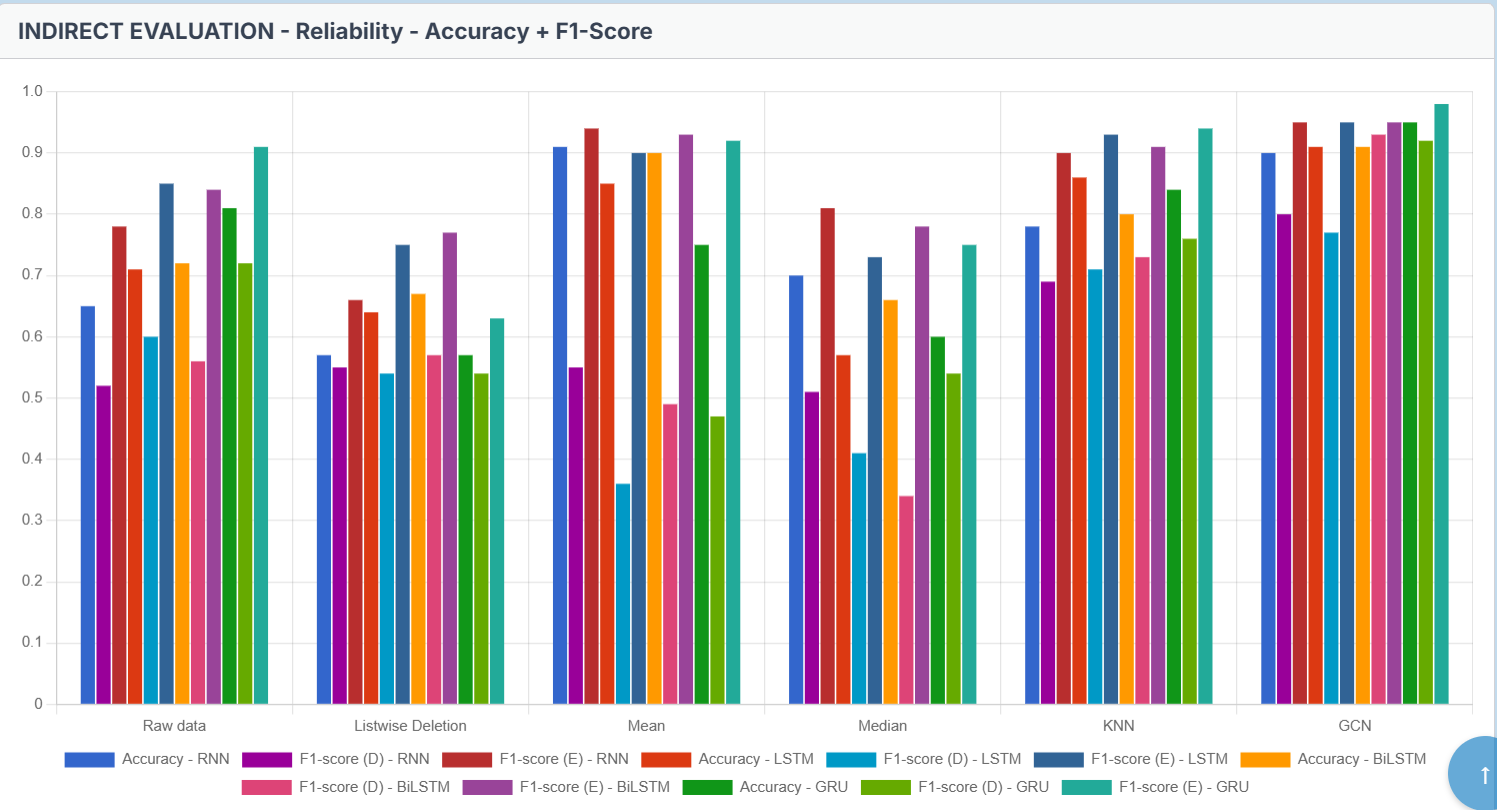
\includegraphics[width=\textwidth]{imgs/demo-indirect.png}
        \label{fig:sub1}
    \end{subfigure}
    \hfill
    \begin{subfigure}[b]{0.45\textwidth}
        \centering
        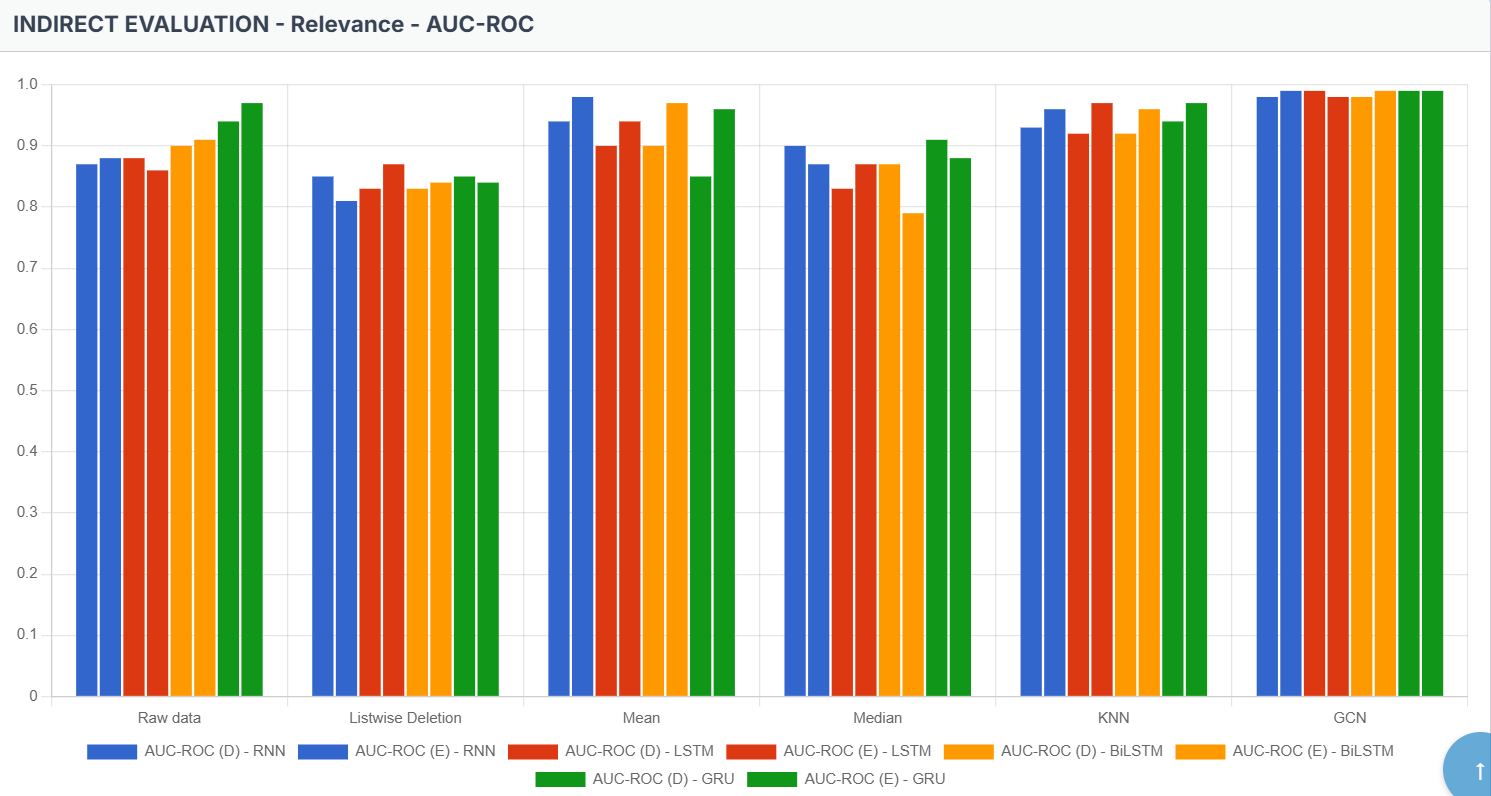
\includegraphics[width=\textwidth]{imgs/demo-indirect-aucroc.png}
        \label{fig:sub2}
    \end{subfigure}
    \caption{Kết quả đo lường chất lượng dữ liệu}
    \label{fig:2images}
\end{figure}


\subsection{Hiệu suất mô hình toàn diện}
\begin{figure}[H]
    \centering
    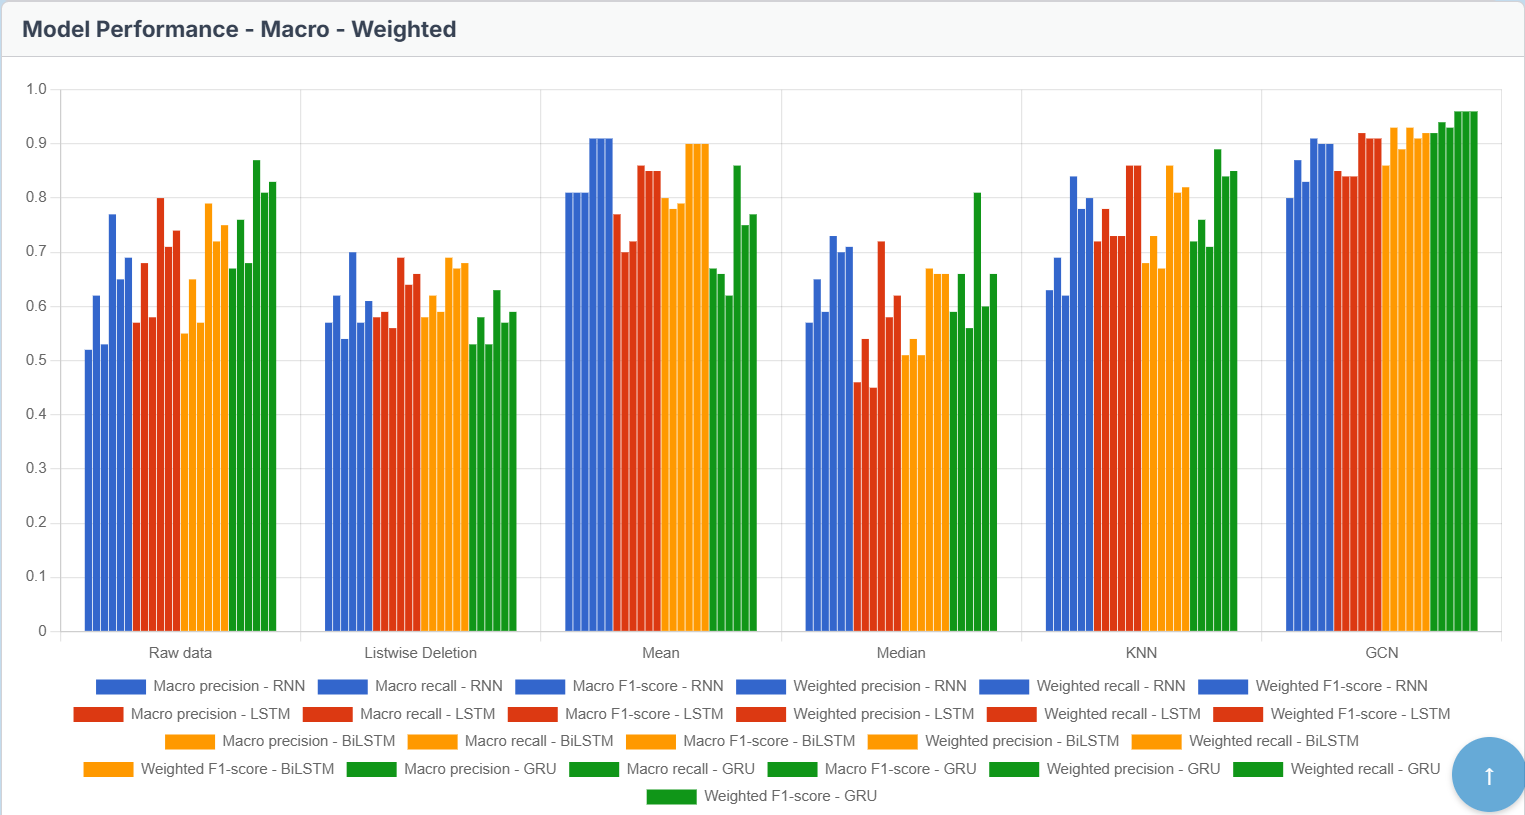
\includegraphics[width = 0.8\textwidth]{imgs/demo-modelperf.png}
    \caption{Biểu đồ so sánh hiệu suất mô hình qua các chỉ số Macro và Weighted}
    \label{fig:demo-modelperf}
\end{figure}

Ngoài ra, các chỉ số đánh giá mức độ trung bình là Macro và Weighted đã được sử dụng nhằm mang lại cái nhìn toàn diện và khách quan để đánh giá mô hình. Phương pháp điền khuyết bằng GCN do chúng tôi đề xuất đã mang lại sự cải thiện rõ rệt và ổn định trên tất cả các mô hình học sâu. Khi áp dụng GCN, mô hình GRU đạt được Macro F1-score cao nhất là 0.93 và Weighted F1-score là 0.96, vô cùng khả quan khi so sánh với các phương pháp khác. Ví dụ, với dữ liệu chưa xử lý, GRU chỉ đạt Macro F1-score tối đa 0.68, trong khi BiLSTM còn thấp hơn với 0.59 khi dùng phương pháp loại bỏ hàng bị thiếu. Ngay cả với các kỹ thuật điền khuyết phổ biến như Mean và KNN, kết quả vẫn chưa thể sánh bằng GCN. Cụ thể, Macro F1-score cao nhất của phương pháp Mean là 0.81 (RNN), còn KNN đạt 0.73 (LSTM). Trong khi đó, GCN luôn duy trì mức F1-score trên 0.83 với mọi mô hình được kiểm thử, cho thấy tính hiệu quả và độ ổn định vượt trội.

Sự vượt trội của GCN không chỉ nằm ở việc đạt được các điểm số cao nhất mà còn thể hiện ở tính ổn định và mạnh mẽ trên các kiến trúc mô hình khác nhau như RNN, LSTM, BiLSTM hay GRU.

\begin{sidewaystable}
\centering
\normalsize
\caption{Hiệu suất mô hình theo các chỉ số trung bình Macro và Weighted}
\renewcommand\arraystretch{2.8}
\label{tab:results-table}
\resizebox{\textheight}{!}{ % Mở rộng bảng theo chiều cao giấy
    \begin{tabular}{|c|c|c|c|c|c|c|c|c|c|c|c|c|c|c|c|c|c|c|c|c|c|c|c|c|}
        \hline
        \multirow{3}{*}{\textbf{Dataset}} & \multicolumn{12}{c|}{\textbf{Macro}} & \multicolumn{12}{c|}{\textbf{Weighted}} \\
        \cline{2-25}
        & \multicolumn{4}{c|}{\textbf{Macro Precision}} & \multicolumn{4}{c|}{\textbf{Macro Recall}} & \multicolumn{4}{c|}{\textbf{Macro F1-score}} & \multicolumn{4}{c|}{\textbf{Weighted Precision}} & 
        \multicolumn{4}{c|}{\textbf{Weighted Recall}} & 
        \multicolumn{4}{c|}{\textbf{Weighted F1-score}}\\
        \cline{2-25}
        & RNN &LSTM & BiLSTM & GRU & 
         RNN &LSTM & BiLSTM & GRU & 
          RNN &LSTM & BiLSTM & GRU & 
           RNN &LSTM & BiLSTM & GRU & 
            RNN &LSTM & BiLSTM & GRU & 
             RNN &LSTM & BiLSTM & GRU \\
        \cline{2-25}
        \hline
        Raw data & 0.52 & 0.57 & 0.55 & 0.67 & 0.62 & 0.68 & 0.65 & 0.76 & 0.53 & 0.58 & 0.57 & 0.68 & 0.77 & 0.80 & 0.79 & 0.87 & 0.65 & 0.71 & 0.72 & 0.81 & 0.69 & 0.74 & 0.75 & 0.83\\
        \hline
        Listwise Deletion & 0.57 & 0.58 & 0.58  & 0.53 & 0.62 & 0.59 & 0.62 & 0.58 & 0.54 & 0.56 & 0.59 & 0.53 & 0.70 & 0.69 & 0.69 & 0.63 & 0.57 & 0.64 & 0.67 & 0.57 & 0.61 & 0.66 & 0.68 & 0.59      \\
        \hline
        Mean & 0.81 & 0.77 & 0.80 & 0.67 & 0.81 & 0.70 & 0.78 & 0.66 & 0.81 & 0.72 & 0.79 & 0.62 & 0.91 & 0.86 & 0.90 & 0.86 & 0.91 & 0.85 & 0.90 & 0.75 & 0.91 & 0.85 & 0.90 & 0.77 \\
        \hline
        Median   & 0.57 & 0.46 & 0.51 & 0.59 & 0.65 & 0.54 & 0.54 & 0.66 & 0.59 & 0.45 & 0.51 & 0.56 & 0.73 & 0.72 & 0.67 & 0.81 & 0.70 & 0.57 & 0.66 & 0.60 & 0.71 & 0.62 & 0.66 & 0.66\\
        \hline
        KNN  & 0.63 & 0.72 & 0.68 & 0.72 & 0.69 & 0.78 & 0.73 & 0.76 & 0.62 & 0.73 & 0.67 & 0.71 & 0.84 & 0.73 & 0.86 & 0.89 & 0.78 & 0.86 & 0.81 & 0.84 & 0.80 & 0.86 & 0.82 & 0.85 \\
        \hline
        KI  & 0.53 & 0.82 & 0.57 & 0.80 & 0.63 & 0.71 & 0.65 & 0.76 & 0.56 & 0.62 & 0.58 & 0.77 & 0.78 & 0.82 & 0.80 & 0.80 & 0.72 & 0.75 & 0.73 & 0.75 & 0.74 & 0.78 & 0.75 & 0.76 \\
        \hline
        \textbf{GCN}  & \textbf{0.80} & \textbf{0.85} & \textbf{0.86} & \textbf{0.92} & \textbf{0.87} & \textbf{0.84} & \textbf{0.93} & \textbf{0.94} & \textbf{0.83} & \textbf{0.84} & \textbf{0.89} & \textbf{0.93} & \textbf{0.91} & \textbf{0.92} & \textbf{0.93} & \textbf{0.96} & \textbf{0.90} & \textbf{0.91} & \textbf{0.91} &
        \textbf{0.96} & \textbf{0.90} & \textbf{0.91} & \textbf{0.92} & \textbf{0.96}  \\
        \hline
    \end{tabular}
}
\end{sidewaystable}



% \renewcommand\arraystretch{2.8}
% \begin{sidewaystable} 
% \centering
% \normalsize
% \caption{So sánh hiệu quả phương pháp điền khuyết KI vs GCN-I}
% \label{tab:results-table-quality-knn-gcn}
% \resizebox{\textheight}{!}{
%     \begin{tabular}{|c|c|c|c|c|c|c|c|c|c|c|c|c|c|c|c|c|c|c|c|c|c|c|}
%         \hline
%         \multirow{4}{*}{\textbf{Dataset}} & \multicolumn{2}{c|}{\textbf{Direct Evaluation}} & \multicolumn{20}{c|}{\textbf{Indirect Evaluation}} \\
%         \cline{2-23}
%         & \multirow{2}{*}{\textbf{Completeness}} & \multirow{2}{*}{\textbf{Consistency}} & \multicolumn{12}{c|}{\textbf{Reliability}} & \multicolumn{8}{c|}{\textbf{Relevance}}\\
%         \cline{4-23}
%         & & &\multicolumn{4}{c|}{Accuracy} & \multicolumn{8}{c|}{F1-Score} & \multicolumn{8}{c|}{AUC-ROC} \\
%         \cline{4-23}
%         & & & \multirow{2}{*} {RNN} & \multirow{2}{*} {LSTM} & \multirow{2}{*} {BiLSTM} & \multirow{2}{*} {GRU} & \multicolumn{4}{c|}{Label D} & \multicolumn{4}{c|}{Label E} & \multicolumn{4}{c|}{Label D} & \multicolumn{4}{c|}{Label E}\\ 
%         \cline{8-23}
%         & & & &  & & & RNN & LSTM & BiLSTM & GRU & RNN & LSTM & BiLSTM & GRU & RNN & LSTM & BiLSTM & GRU & RNN & LSTM & BiLSTM & GRU \\
%         \cline{7-23}
%         \hline
%         KI  & 100\% & 99.77\% & 0.72 & 0.76 & 0.73 & 0.75 & 0.56 & 0.60 & 0.57 & 0.62 & 0.85 & 0.87 & 0.86 & 0.86 & 0.87 & 0.89 & 0.90 & 0.87 & 0.91 & 0.92 & 0.91 & 0.91 \\
%         \hline
%         \textbf{GCN}  & 100\% & 100\% & \textbf{0.90} & \textbf{0.91} & \textbf{0.91} & \textbf{0.95} & \textbf{0.80} & \textbf{0.77} & \textbf{0.93} & \textbf{0.92} & \textbf{0.95} & \textbf{0.95} & \textbf{0.95} & \textbf{0.98} & \textbf{0.99} & \textbf{0.98} & \textbf{0.99} & \textbf{0.99} & \textbf{0.98} & \textbf{0.98} & \textbf{0.99} & \textbf{0.99}  \\
%         \hline
%     \end{tabular}
% }
% \end{sidewaystable}


% \begin{sidewaystable}
% \centering
% \normalsize
% \caption{Hiệu suất mô hình theo các chỉ số trung bình Macro và Weighted của phương pháp KI vs GCN-I}
% \renewcommand\arraystretch{2.8}
% \label{tab:results-table-knn-gcn}
% \resizebox{\textheight}{!}{
%     \begin{tabular}{|c|c|c|c|c|c|c|c|c|c|c|c|c|c|c|c|c|c|c|c|c|c|c|c|c|}
%         \hline
%         \multirow{3}{*}{\textbf{Dataset}} & \multicolumn{12}{c|}{\textbf{Macro}} & \multicolumn{12}{c|}{\textbf{Weighted}} \\
%         \cline{2-25}
%         & \multicolumn{4}{c|}{\textbf{Macro Precision}} & \multicolumn{4}{c|}{\textbf{Macro Recall}} & \multicolumn{4}{c|}{\textbf{Macro F1-score}} & \multicolumn{4}{c|}{\textbf{Weighted Precision}} & 
%         \multicolumn{4}{c|}{\textbf{Weighted Recall}} & 
%         \multicolumn{4}{c|}{\textbf{Weighted F1-score}}\\
%         \cline{2-25}
%         & RNN &LSTM & BiLSTM & GRU & 
%          RNN &LSTM & BiLSTM & GRU & 
%           RNN &LSTM & BiLSTM & GRU & 
%            RNN &LSTM & BiLSTM & GRU & 
%             RNN &LSTM & BiLSTM & GRU & 
%              RNN &LSTM & BiLSTM & GRU \\
%         \cline{2-25}
%         \hline
%         KI  & 0.53 & 0.82 & 0.57 & 0.80 & 0.63 & 0.71 & 0.65 & 0.76 & 0.56 & 0.62 & 0.58 & 0.77 & 0.78 & 0.82 & 0.80 & 0.80 & 0.72 & 0.75 & 0.73 & 0.75 & 0.74 & 0.78 & 0.75 & 0.76 \\
%         \hline
%         \textbf{GCN}  & \textbf{0.80} & \textbf{0.85} & \textbf{0.86} & \textbf{0.92} & \textbf{0.87} & \textbf{0.84} & \textbf{0.93} & \textbf{0.94} & \textbf{0.83} & \textbf{0.84} & \textbf{0.89} & \textbf{0.93} & \textbf{0.91} & \textbf{0.92} & \textbf{0.93} & \textbf{0.96} & \textbf{0.90} & \textbf{0.91} & \textbf{0.91} &
%         \textbf{0.96} & \textbf{0.90} & \textbf{0.91} & \textbf{0.92} & \textbf{0.96}  \\
%         \hline
%     \end{tabular}
% }
% \end{sidewaystable}



\chapter{SmartEduTrack: Hệ thống theo dõi học tập thông minh hỗ trợ ra quyết định quản lý}
\label{chap:chap6}
\section{Giới thiệu SmartEduTrack}
SmartEduTrack là một nền tảng website giúp người quản lý khóa học giám sát học viên. Xuất phát từ một dự án nghiên cứu về ứng dụng Deep Learning trong giáo dục, chúng tôi đã phát triển SmartEduTrack nhằm hiện thực hóa tiềm năng của AI trong giáo dục trực tuyến.

Website có các chức năng giúp theo dõi hiệu suất học viên, giúp người quản lý có được những kế hoạch và giải pháp kịp thời. Điểm đặc biệt của SmartEduTrack là việc tích hợp một mô hình có thể dự đoán khả năng hoàn thành khóa học của từng học viên chỉ trong 3 tuần đầu kể từ khi người học bắt đầu. Điều này giúp các nhà quản lý phát hiện kịp thời những học viên có nguy cơ gặp khó khăn hoặc bỏ học, từ đó cung cấp sự hỗ trợ cá nhân hóa và can thiệp sớm, tối ưu hóa cơ hội thành công cho tất cả người học.
\section{Phân tích thiết kế}
 \textbf{SmartEduTrack} được phân tích thiết kế để đáp ứng các mục tiêu chính bao gồm:

\begin{itemize}
    \item Đưa ra dự đoán chuẩn xác về kết quả học tập của người học ngay trong những tuần đầu của khóa học.
    \item Cung cấp giao diện trực quan, thân thiện với các chức năng hữu ích nhằm hỗ trợ tối đa cho người quản lý khóa học.

\end{itemize}

SmartEduTrack được thiết kế với các chức năng cốt lõi tập trung phục vụ một nhóm người dùng duy nhất, đó là \textbf{người quản lý khóa học}.

\begin{table}[H]
\centering
\caption{Bảng Use Case của hệ thống SmartEduTrack}
\label{tab:usecase}
\renewcommand{\arraystretch}{1.2} % tăng độ cao dòng
\begin{tabular}{|c|p{5cm}|p{3cm}|p{4.5cm}|}
\hline
\multicolumn{1}{|c|}{\textbf{STT}} & \multicolumn{1}{c|}{\textbf{Use Case}} & \multicolumn{1}{c|}{\textbf{Tác nhân}} & \multicolumn{1}{c|}{\textbf{Trang}} \\
\hline
1 & Xem danh sách người học & Course assistant & Education Management \\
\hline
2 & Bộ lọc người học theo khóa học hoặc tháng/năm đăng ký khóa học & Course assistant & Education Management \\
\hline
3 & Xem chi tiết hành vi người học & Course assistant & Education Management \\
\hline
4 & Xem xu hướng học tập của người học & Course assistant & Education Management \\
\hline
5 & Dự đoán kết quả hoàn thành khóa học & Course assistant & Education Management \\
\hline
6 & Xuất report & Course assistant & Education Management \\
\hline
7 & Xem danh sách 5 khóa học ghi nhận số người học bỏ dở nhiều nhất & Course assistant & Education Management \\
\hline
8 & Xem tổng quát bộ dữ liệu MOOCs & Course assistant & Overview \\
\hline
9 & Xem chi tiết từng file dữ liệu MOOCs & Course assistant & Overview \\
\hline
10 & Xem tỷ lệ khuyết của từng file dữ liệu & Course assistant & Overview \\
\hline
11 & Xem chi tiết mô tả bộ dữ liệu hành vi người học & Course assistant & Data Quality \\
\hline
12 & Xem số lượng và tỉ lệ nhãn được dự đoán cho từng người học & Course assistant & Data Quality \\
\hline
13 & Xem chất lượng dữ liệu theo độ đo completeness và consisitency & Course assistant & Data Quality \\
\hline
14 & Bộ lọc xem hiệu suất dự đoán của từng mô hình & Course assistant & Data Quality \\
\hline
\end{tabular}
\end{table}


\section{Kiến trúc hệ thống}
% Front-end, Backend: Sử dụng ngôn ngữ gì, có chức năng gì, sử dụng database gì
\begin{figure}[H]
    \centering
    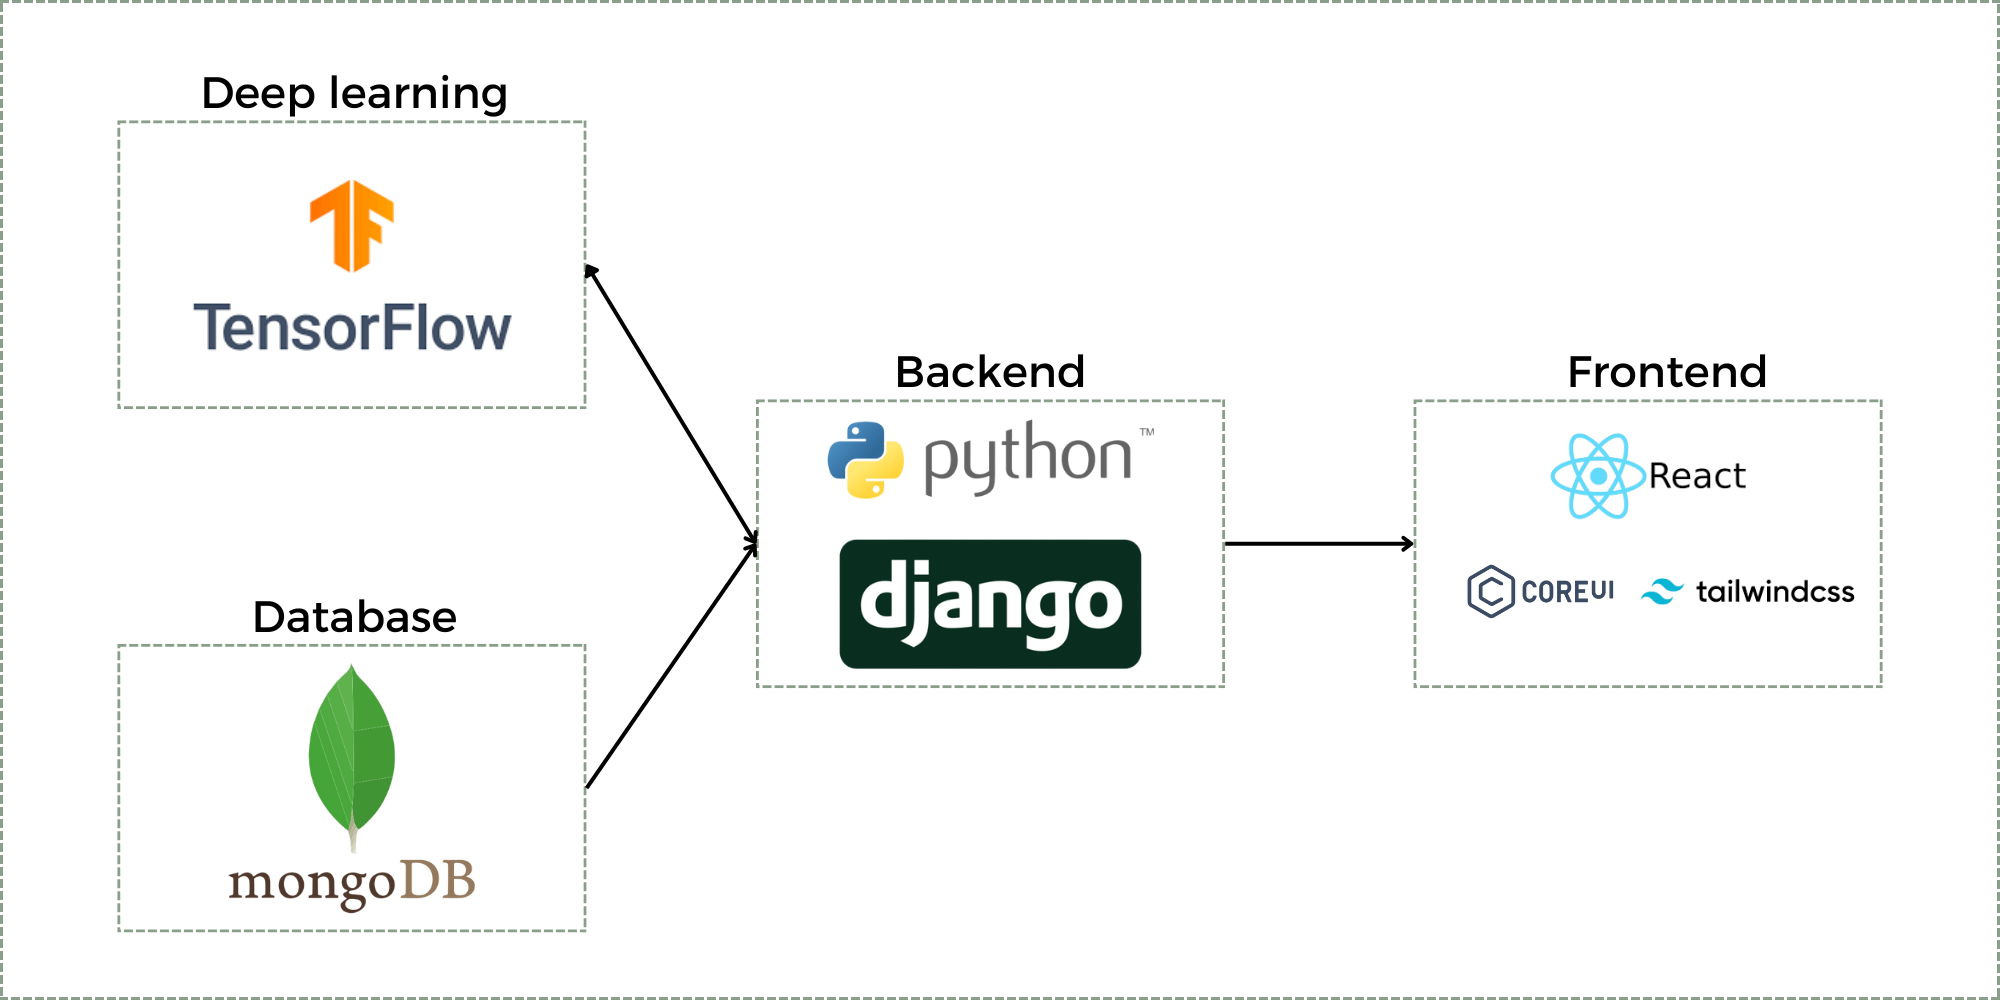
\includegraphics[width = 0.8\textwidth]{imgs/website-system-architecture.png}
    \caption{Kiến trúc hệ thống website SmartEduTrack}
    \label{fig:website-system-architecture}
\end{figure}
SmartEduTrack phát triển dựa trên cấu trúc \textbf{Client-Server}. Mỗi lớp có một nhiệm vụ chuyên biệt và tương tác với nhau qua các giao diện được định nghĩa rõ ràng:

\begin{itemize}
    \item \textbf{Lớp giao diện người dùng (Frontend):} Xây dựng bằng \textit{ReactJS} và \textit{TailwindCSS} để tạo ra một giao diện trực quan, đáp ứng nhanh và thân thiện.
    
    \item \textbf{Lớp xử lý nghiệp vụ (Backend):} Nền tảng Python được sử dụng thông qua framework Django. Nhiệm vụ chính của nó bao gồm xử lý các yêu cầu từ phía giao diện, trao đổi thông tin với database và tích hợp mô hình học sâu để thực hiện dự đoán kết quả hoàn thành khóa học.
    
    \item \textbf{Lớp dữ liệu (Database):} Lớp này sử dụng \textit{MongoDB} làm hệ quản trị cơ sở dữ liệu NoSQL, có nhiệm vụ lưu trữ và quản lý toàn bộ dữ liệu của hệ thống. Dữ liệu này bao gồm hồ sơ chi tiết của học viên, dữ liệu quá trình tương tác học tập, và các kết quả dự đoán được tạo ra bởi mô hình.
\end{itemize}

\section{SmartEduTrack - Demo}
% chụp hình giới thiệu trang web
\subsection{Chức năng: Xem danh sách người học}
\begin{figure}[H]
    \centering
    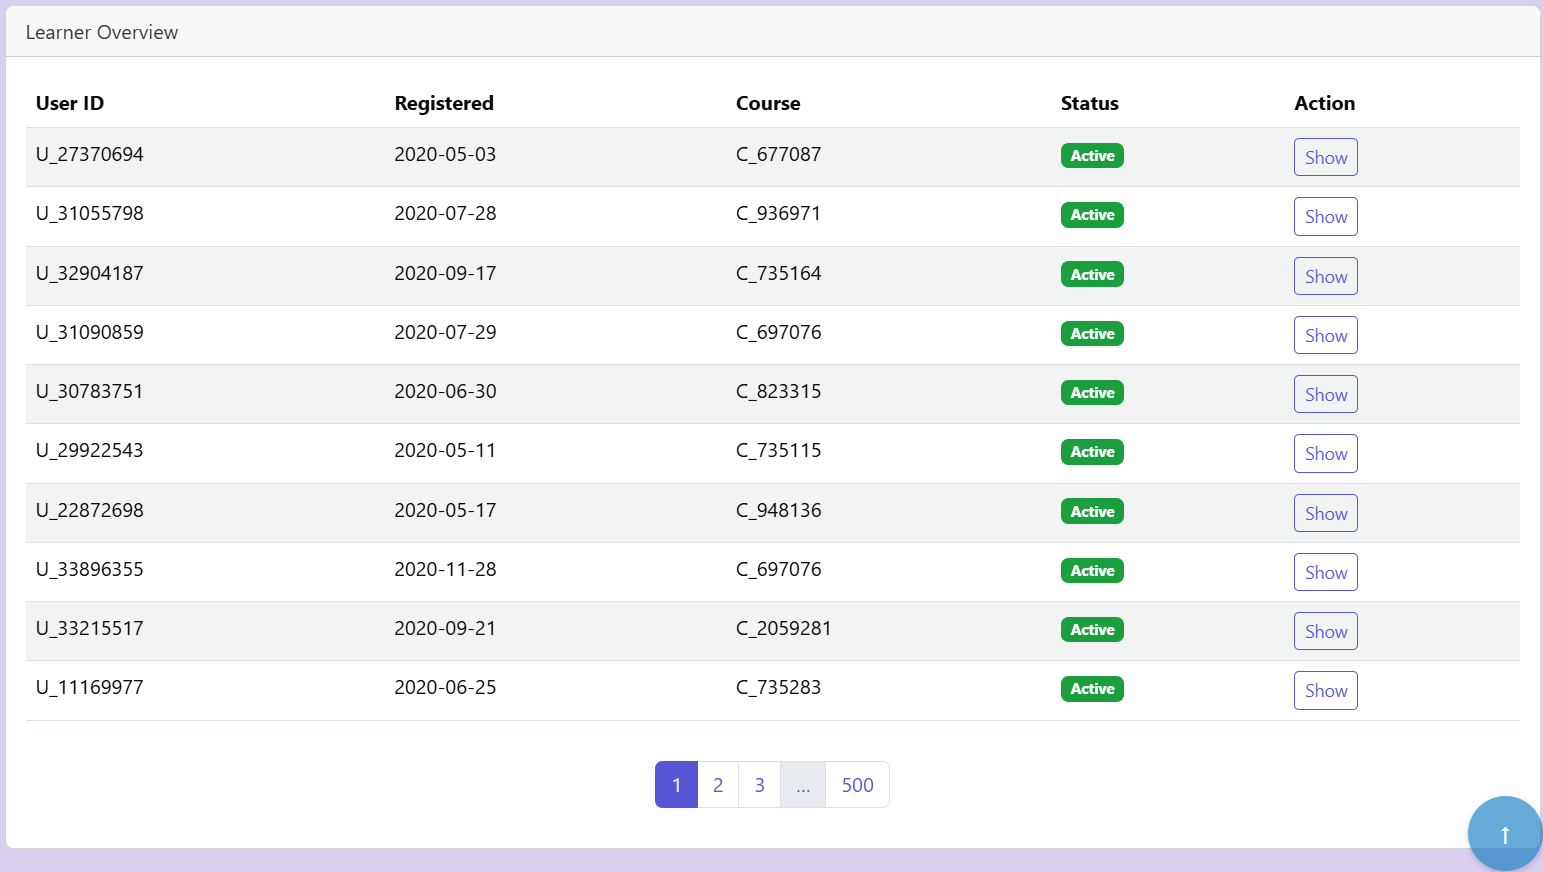
\includegraphics[width = 0.8\textwidth]{imgs/demo-1.png}
    \caption{Danh sách người học}
    \label{fig:demo-1}
\end{figure}
\subsection{Chức năng: Lọc người học theo khóa học hoặc tháng/năm đăng ký khóa học}
\begin{figure}[H]
    \centering
    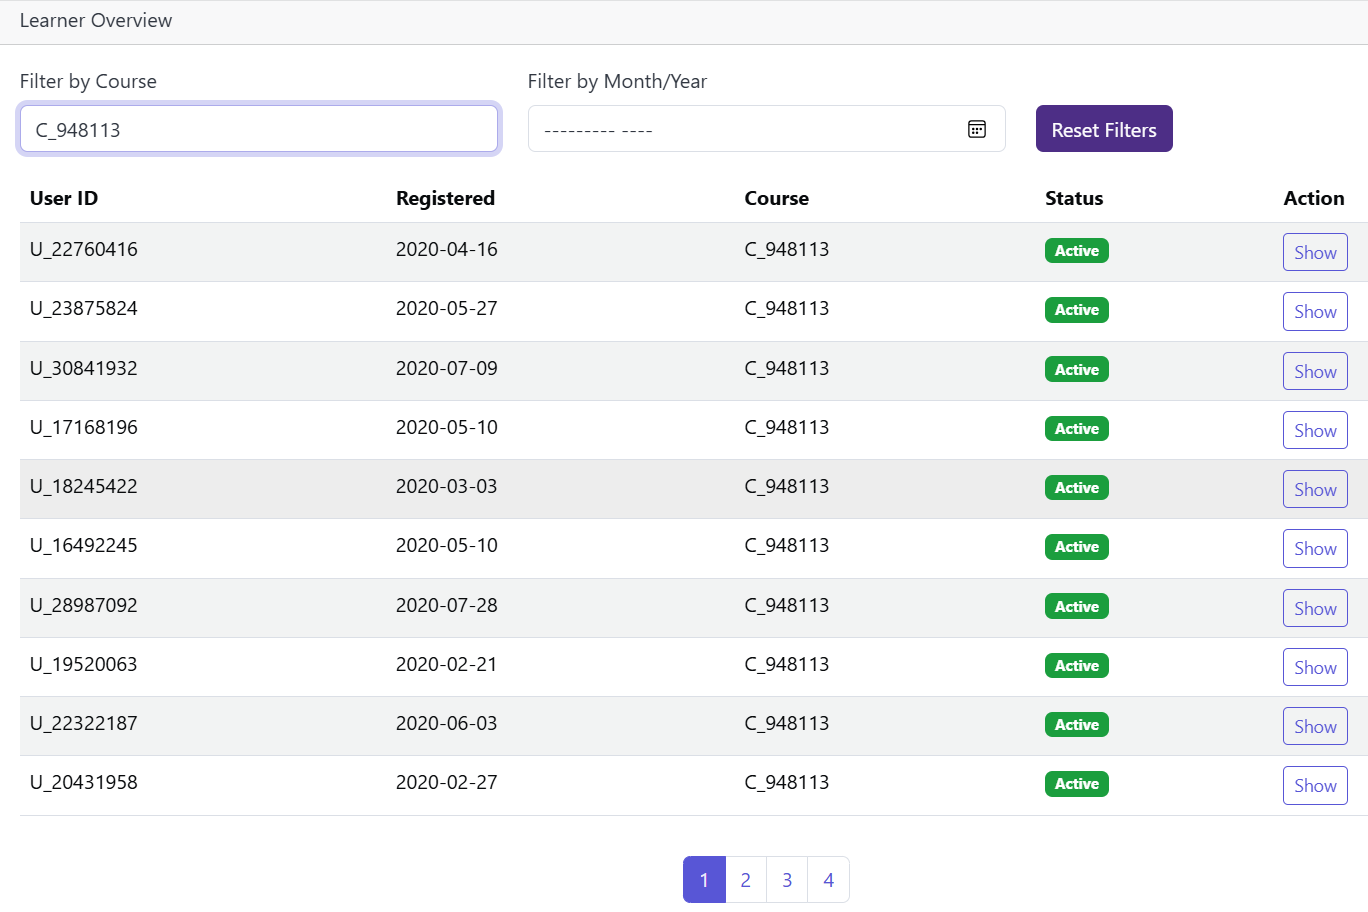
\includegraphics[width = 0.8\textwidth]{imgs/demo-filter.png}
    \caption{Bộ lọc theo khóa học và tháng/năm đăng ký khóa học}
    \label{fig:demo-filter}
\end{figure}
\subsection{Chức năng: Dự đoán kết quả hoàn thành khóa học và xem chi tiết hành vi người học}
\begin{figure}[H]
    \centering
    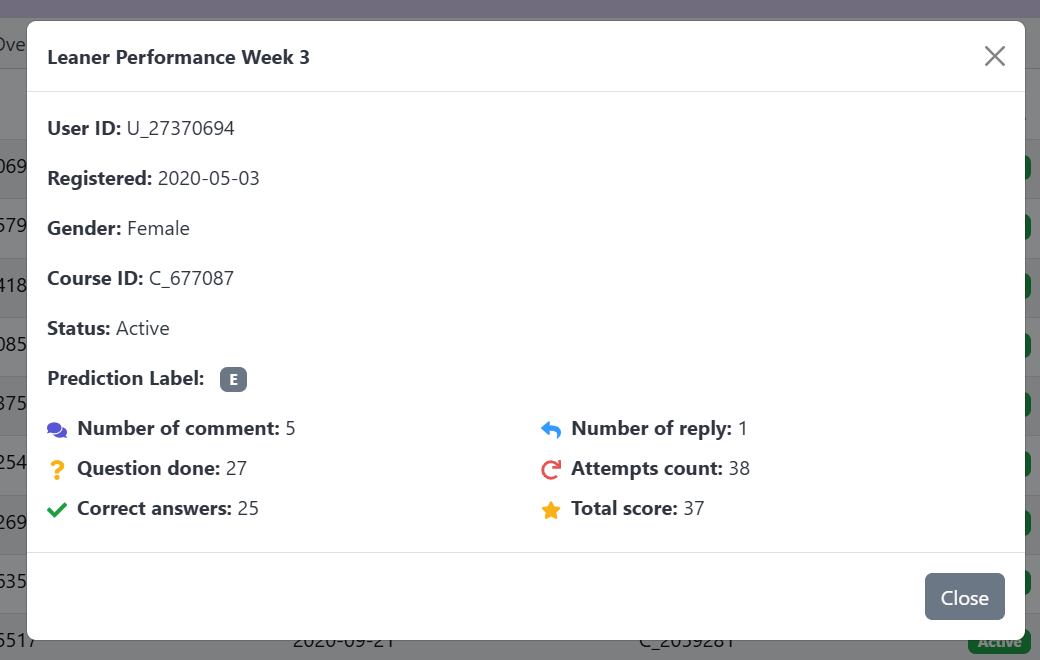
\includegraphics[width = 0.8\textwidth]{imgs/demo-2.png}
    \caption{Dự đoán kết quả hoàn thành khóa học và xem chi tiết hành vi người học}
    \label{fig:demo-2}
\end{figure}
\subsection{Chức năng: Xem xu hướng học tập của người học}
\begin{figure}[H]
    \centering
    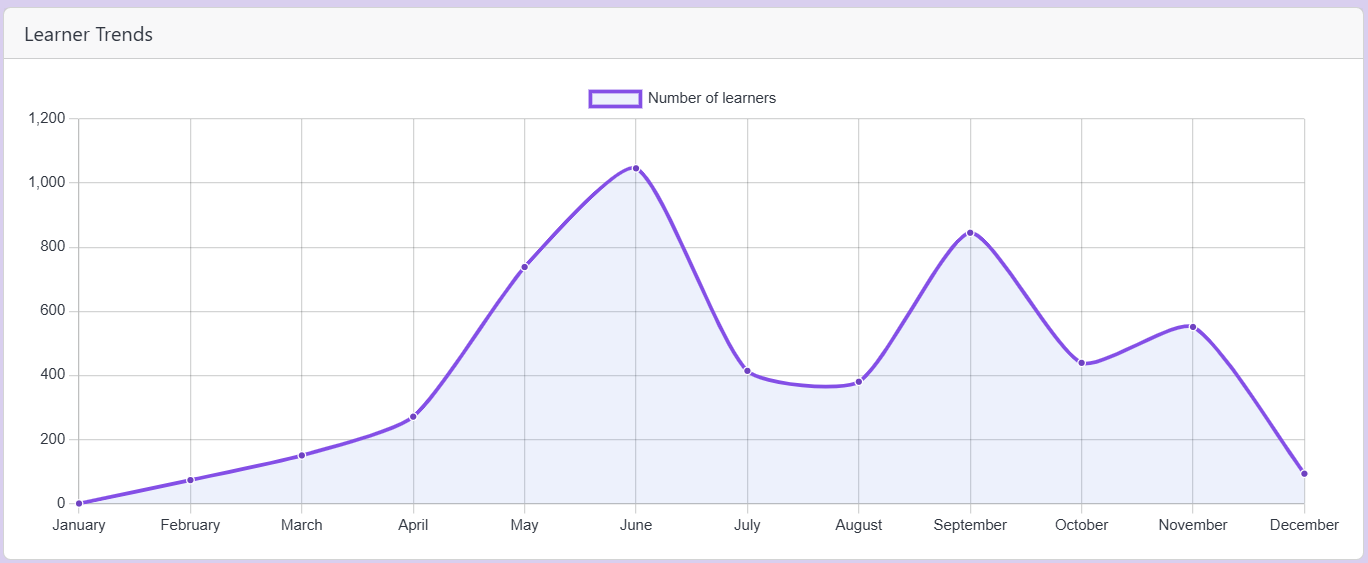
\includegraphics[width = 0.8\textwidth]{imgs/demo-3.png}
    \caption{Xu hướng học tập của người học}
    \label{fig:demo-3}
\end{figure}
\subsection{Chức năng: Xem danh sách 5 khóa học ghi nhận số người học bỏ dở nhiều nhất}
\begin{figure}[H]
    \centering
    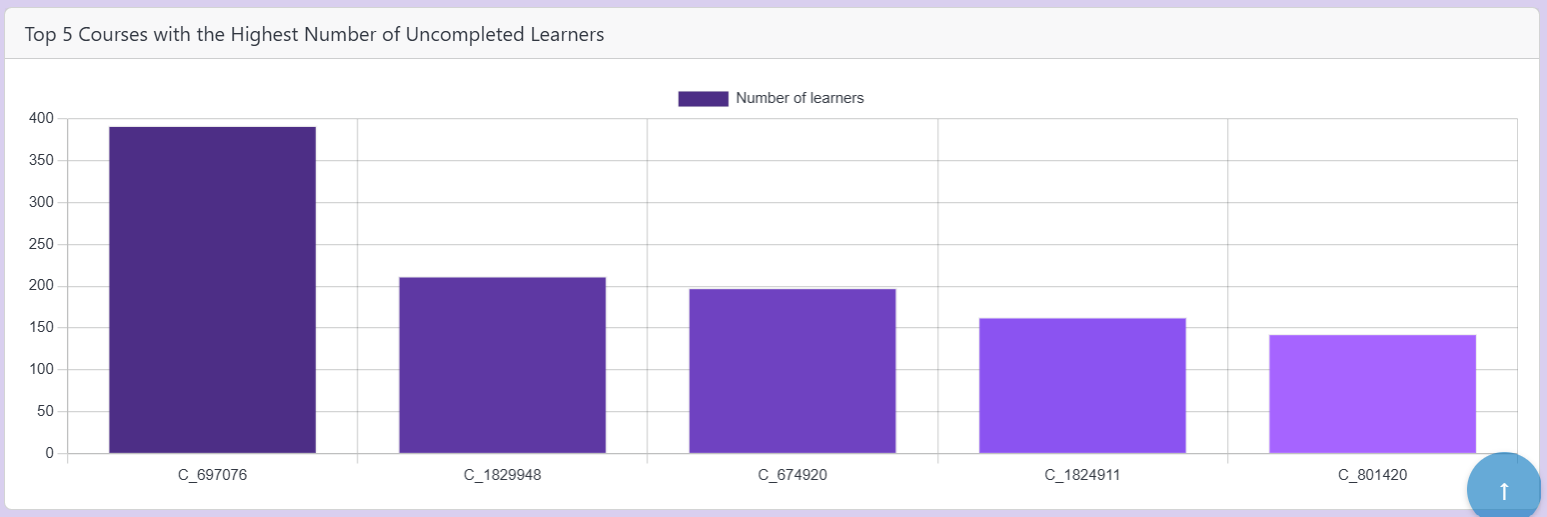
\includegraphics[width = 0.8\textwidth]{imgs/demo-4.png}
    \caption{Danh sách 5 khóa học ghi nhận số người học bỏ dở nhiều nhất}
    \label{fig:demo-4}
\end{figure}
\subsection{Chức năng: Xuất report}
\begin{figure}[H]
    \centering
    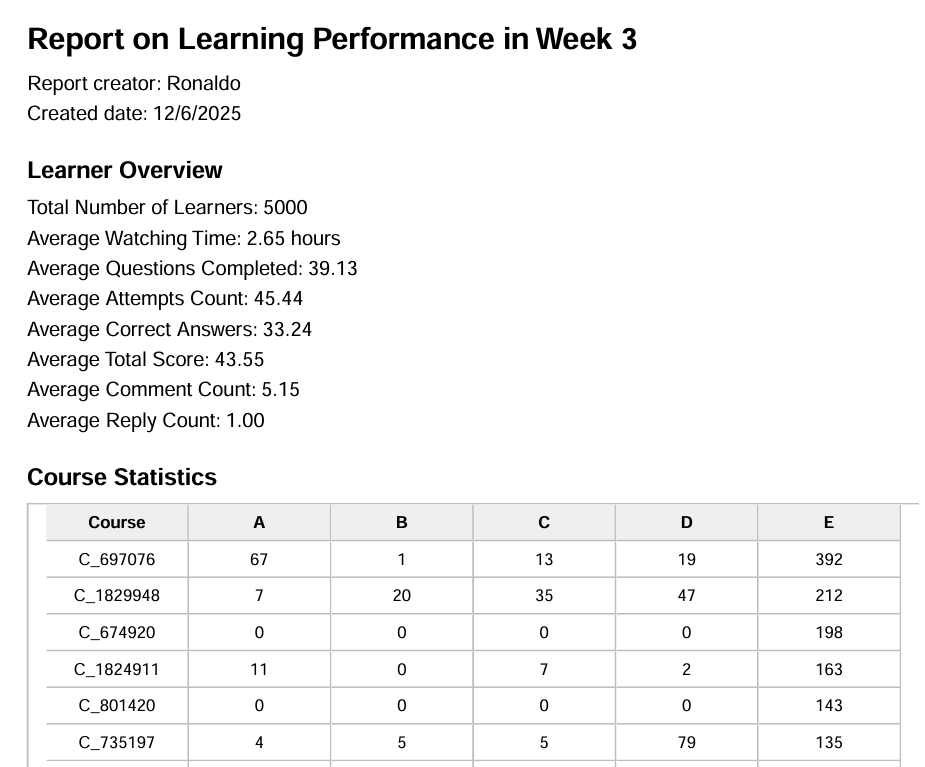
\includegraphics[width = 0.8\textwidth]{imgs/demo-5.png}
    \caption{Mẫu report}
    \label{fig:demo-5}
\end{figure}
\subsection{Chức năng: Xem tổng quát bộ dữ liệu MOOCs}
\begin{figure}[H]
    \centering
    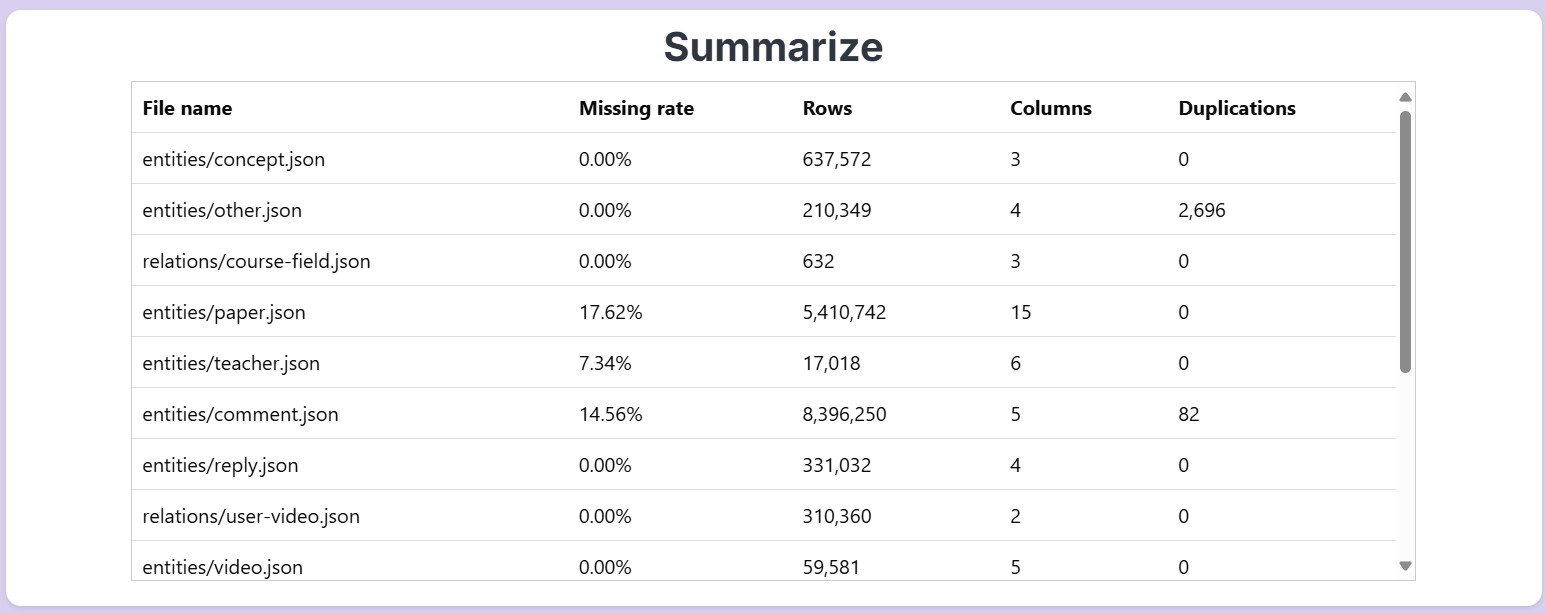
\includegraphics[width = 0.8\textwidth]{imgs/demo-7.png}
    \caption{Tổng quát bộ dữ liệu MOOCs}
    \label{fig:demo-7}
\end{figure}
\subsection{Chức năng: Xem chi tiết từng file dữ liệu MOOCs}
\begin{figure}[H]
    \centering
    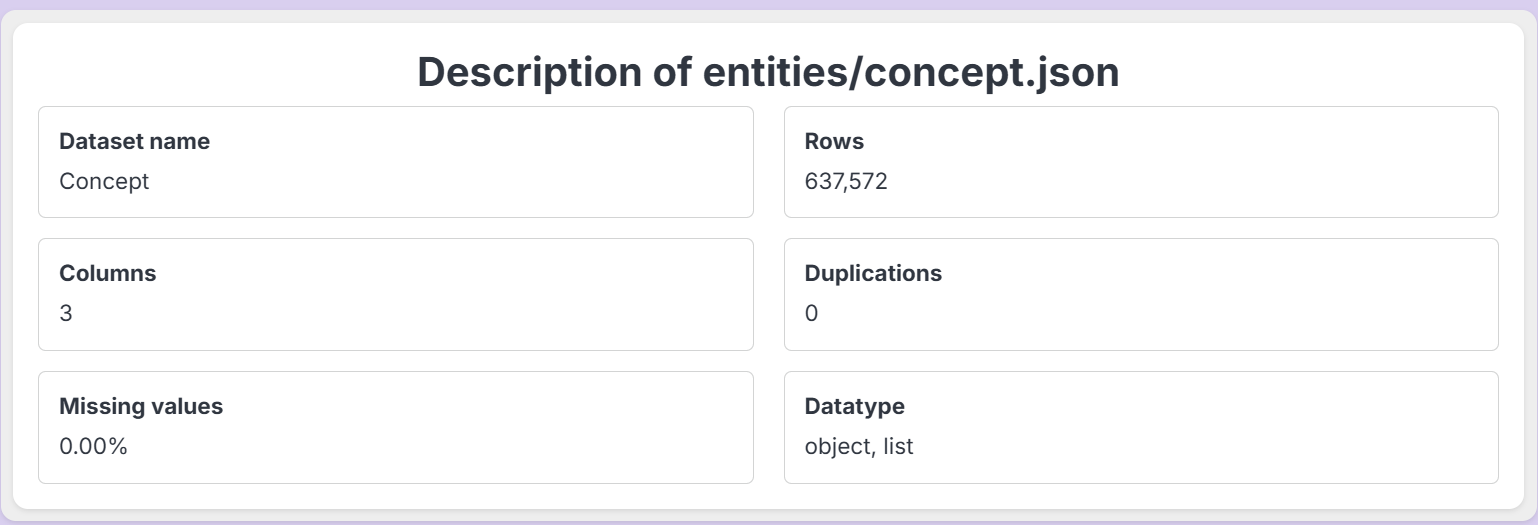
\includegraphics[width = 0.8\textwidth]{imgs/demo-8.png}
    \caption{Chi tiết file dữ liệu concept.json}
    \label{fig:demo-8}
\end{figure}
\subsection{Chức năng: Xem tỷ lệ khuyết của từng file dữ liệu}
\begin{figure}[H]
    \centering
    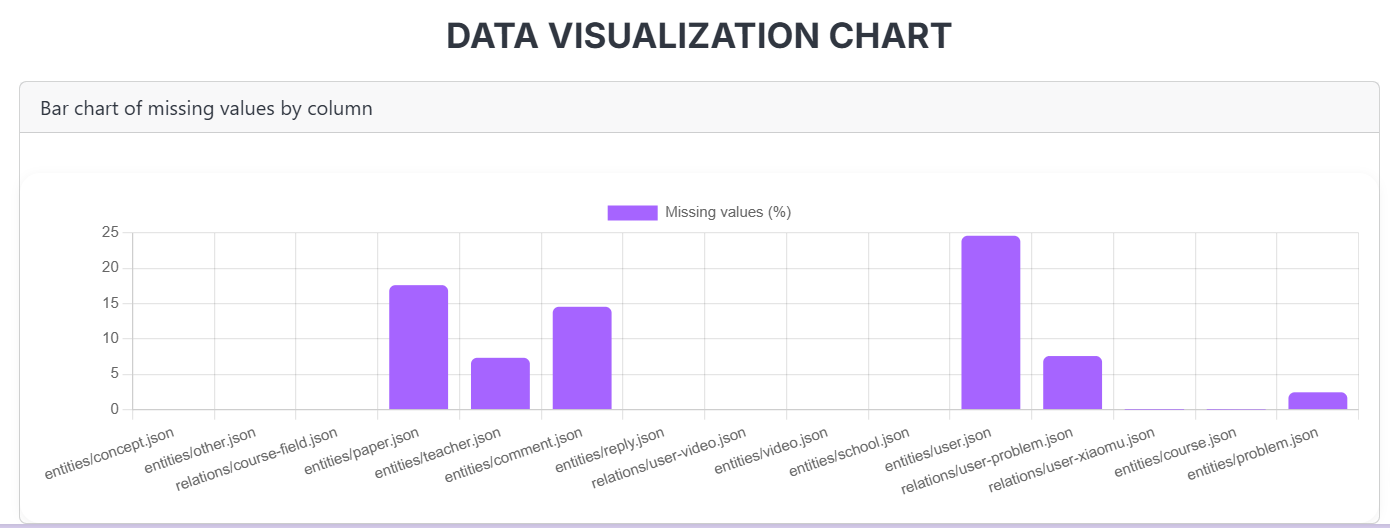
\includegraphics[width = 0.8\textwidth]{imgs/demo-9.png}
    \caption{Biểu đồ tỷ lệ khuyết của từng file dữ liệu}
    \label{fig:demo-9}
\end{figure}
\subsection{Chức năng: Xem chi tiết mô tả bộ dữ liệu hành vi người học}
\begin{figure}[H]
    \centering
    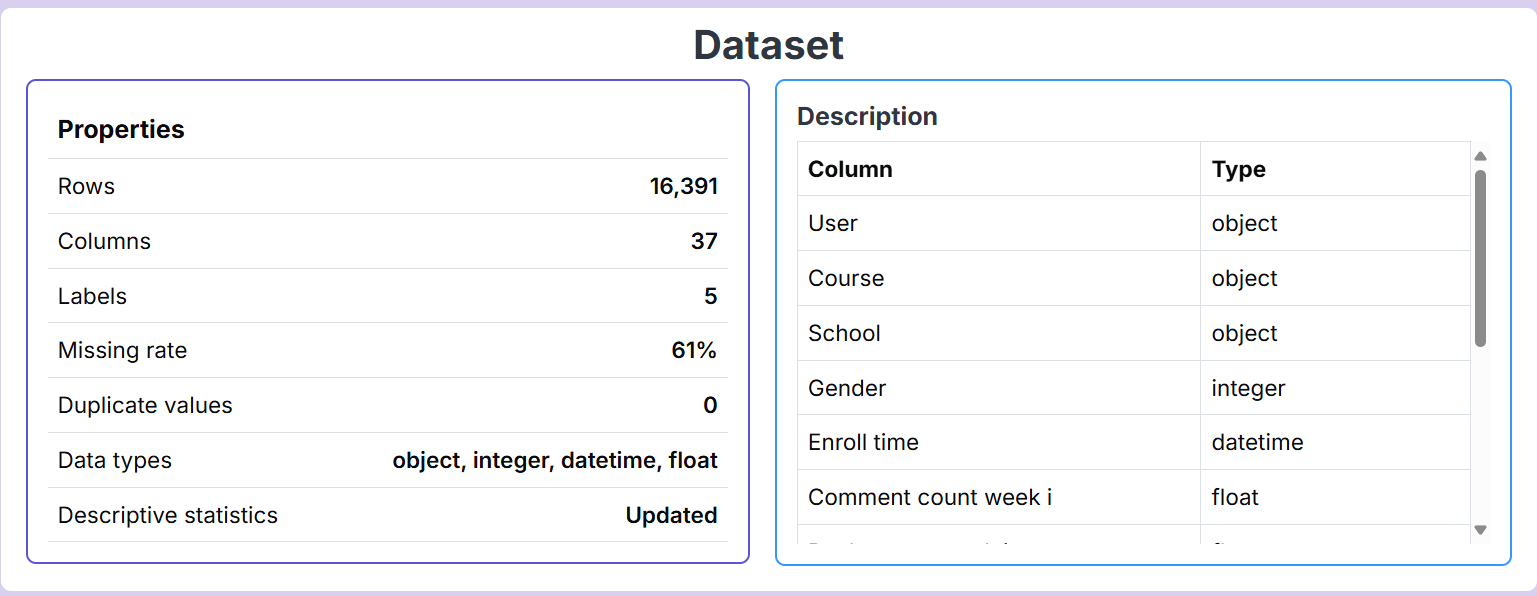
\includegraphics[width = 0.8\textwidth]{imgs/demo-10.png}
    \caption{Mô tả bộ dữ liệu hành vi người học}
    \label{fig:demo-10}
\end{figure}
\subsection{Chức năng: Xem số lượng và tỉ lệ nhãn được dự đoán cho từng người học}
\begin{figure}[H]
    \centering
    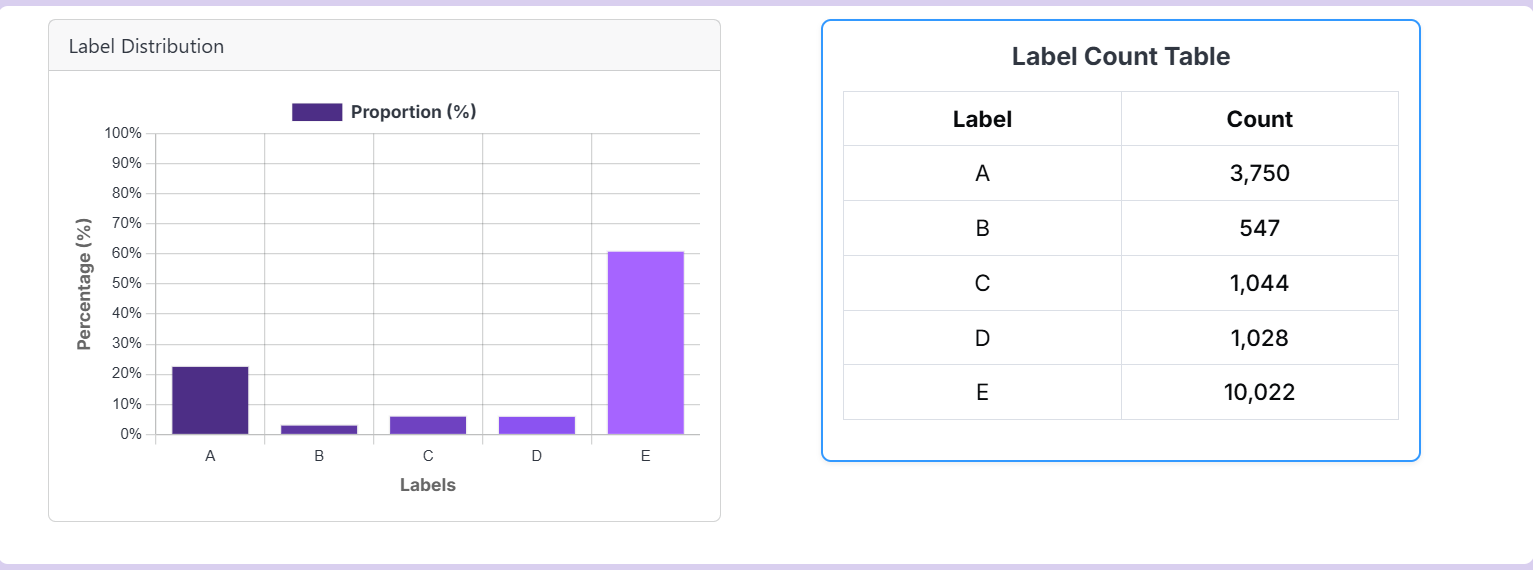
\includegraphics[width = 0.8\textwidth]{imgs/demo-11.png}
    \caption{Biểu đồ tỷ lệ nhãn và bảng số lượng theo từng nhãn}
    \label{fig:demo-11}
\end{figure}
\subsection{Chức năng: Xem chất lượng dữ liệu theo độ đo completeness và consistency}
\begin{figure}[H]
    \centering
    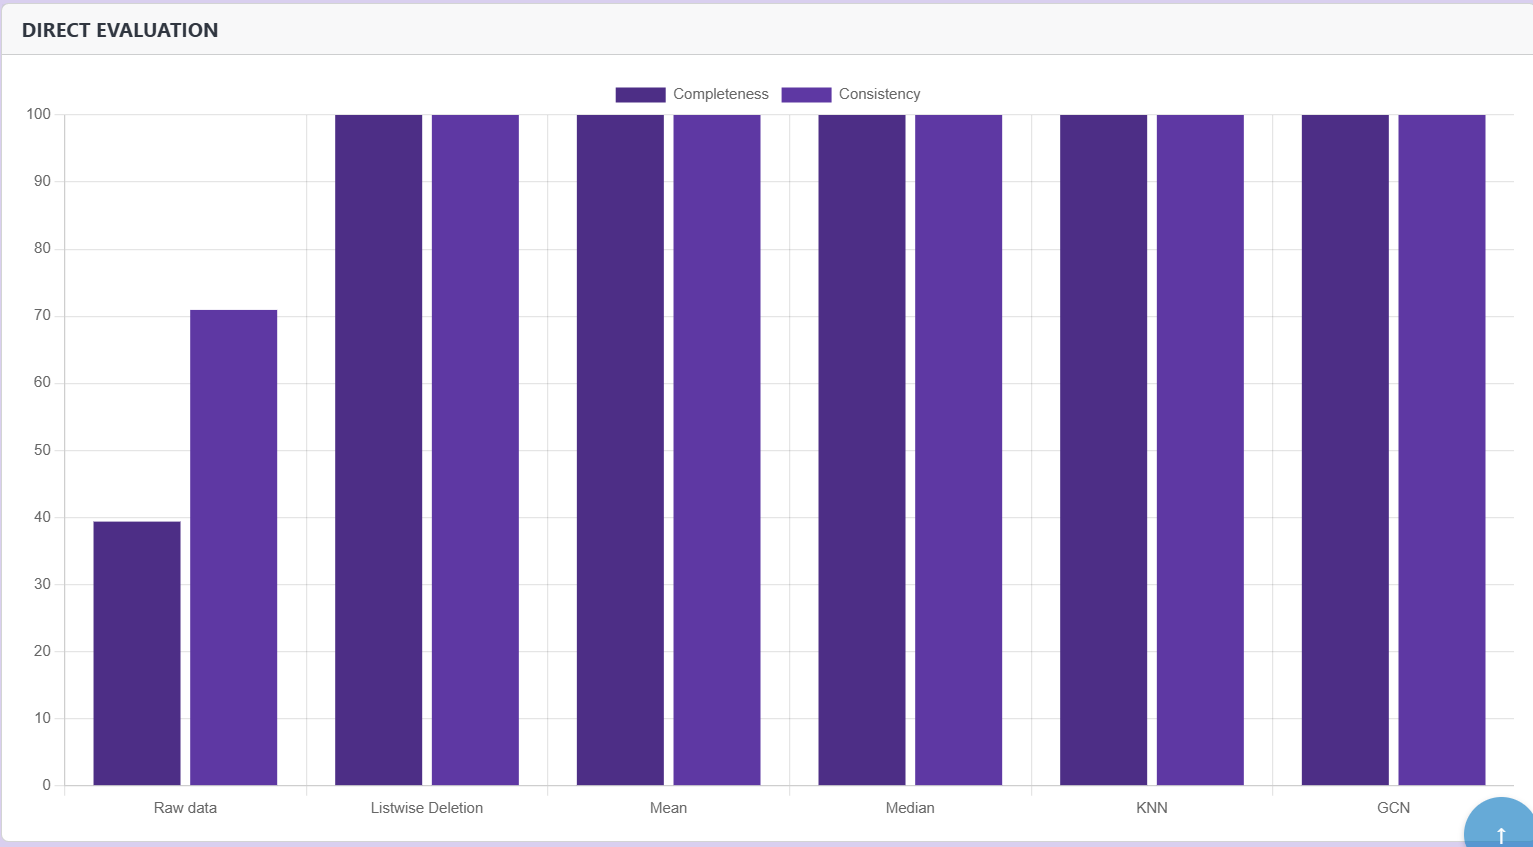
\includegraphics[width = 0.8\textwidth]{imgs/demo-12.png}
    \caption{Biểu đồ chất lượng dữ liệu theo độ đo completeness và consistency}
    \label{fig:demo-12}
\end{figure}
\subsection{Bộ lọc xem hiệu suất dự đoán của từng mô hình}
\begin{figure}[H]
    \centering
    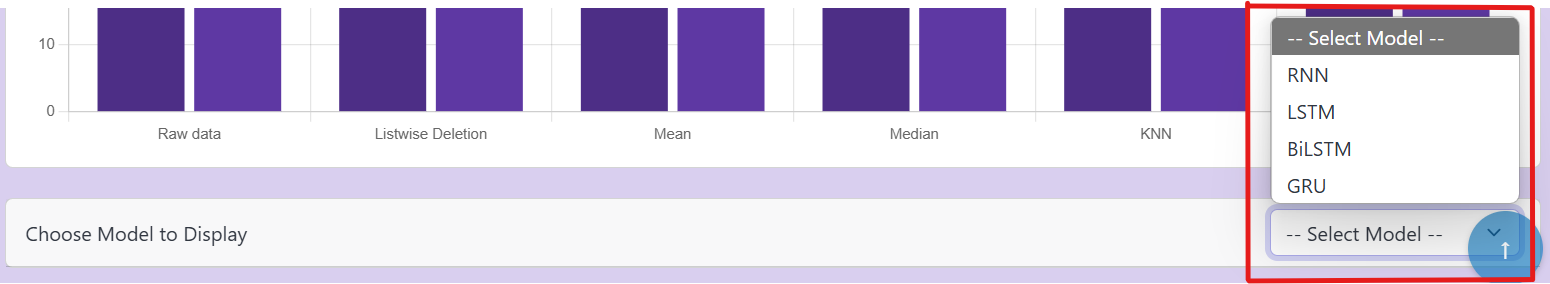
\includegraphics[width = 0.8\textwidth]{imgs/demo-13.png}
    \caption{Bộ lọc kết quả theo mô hình}
    \label{fig:demo-13}
\end{figure}
\begin{figure}[H]
    \centering
    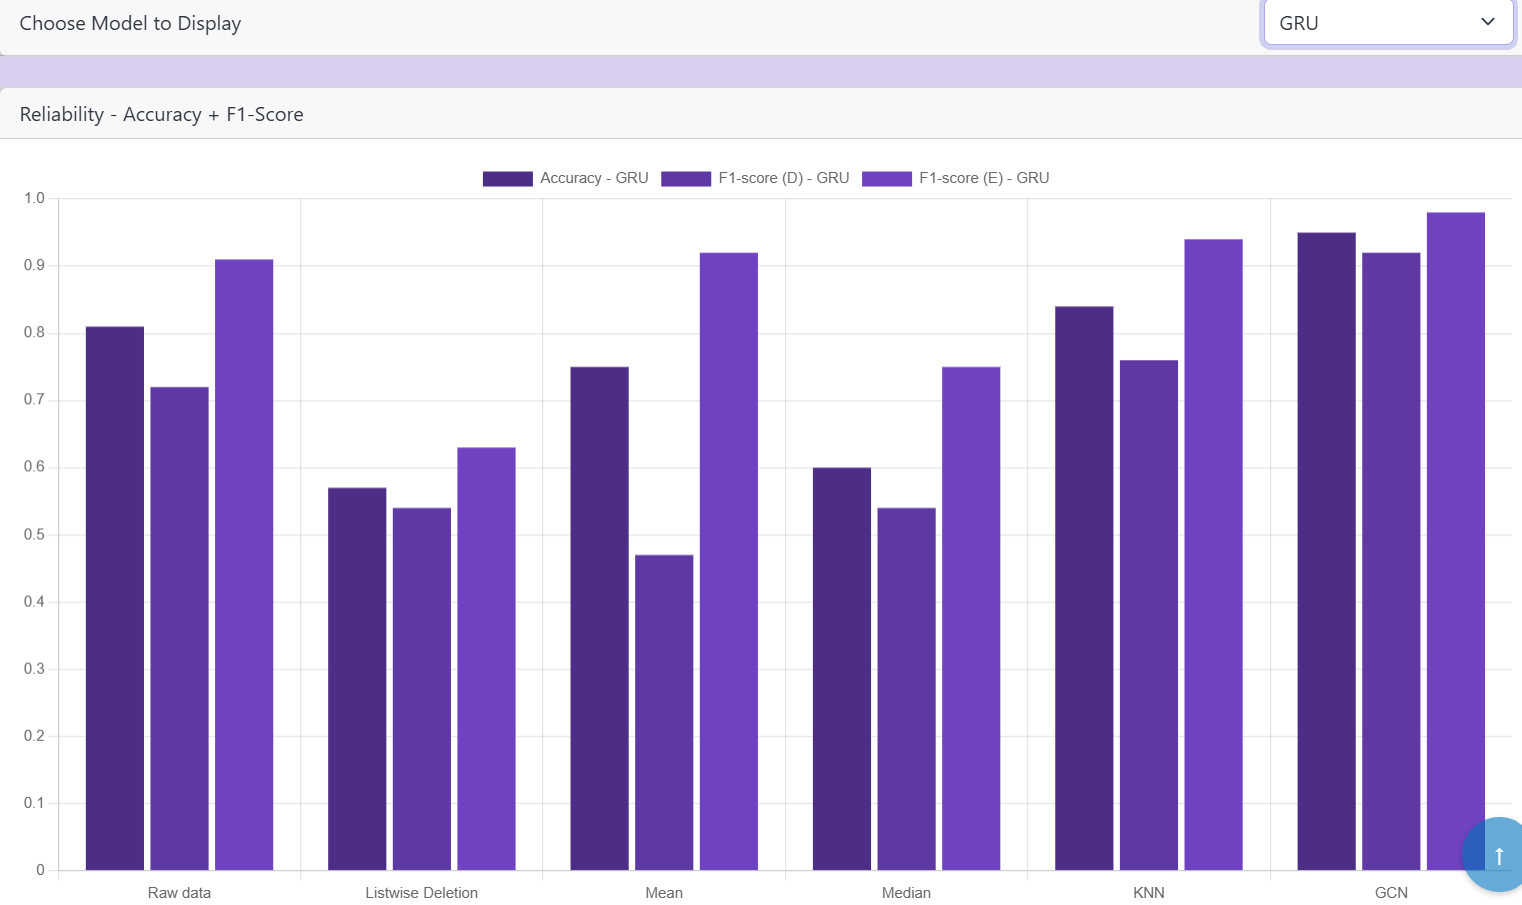
\includegraphics[width = 0.8\textwidth]{imgs/demo-14.png}
    \caption{Accuracy + F1-Score theo mô hình GRU}
    \label{fig:demo-14}
\end{figure}
\begin{figure}[H]
    \centering
    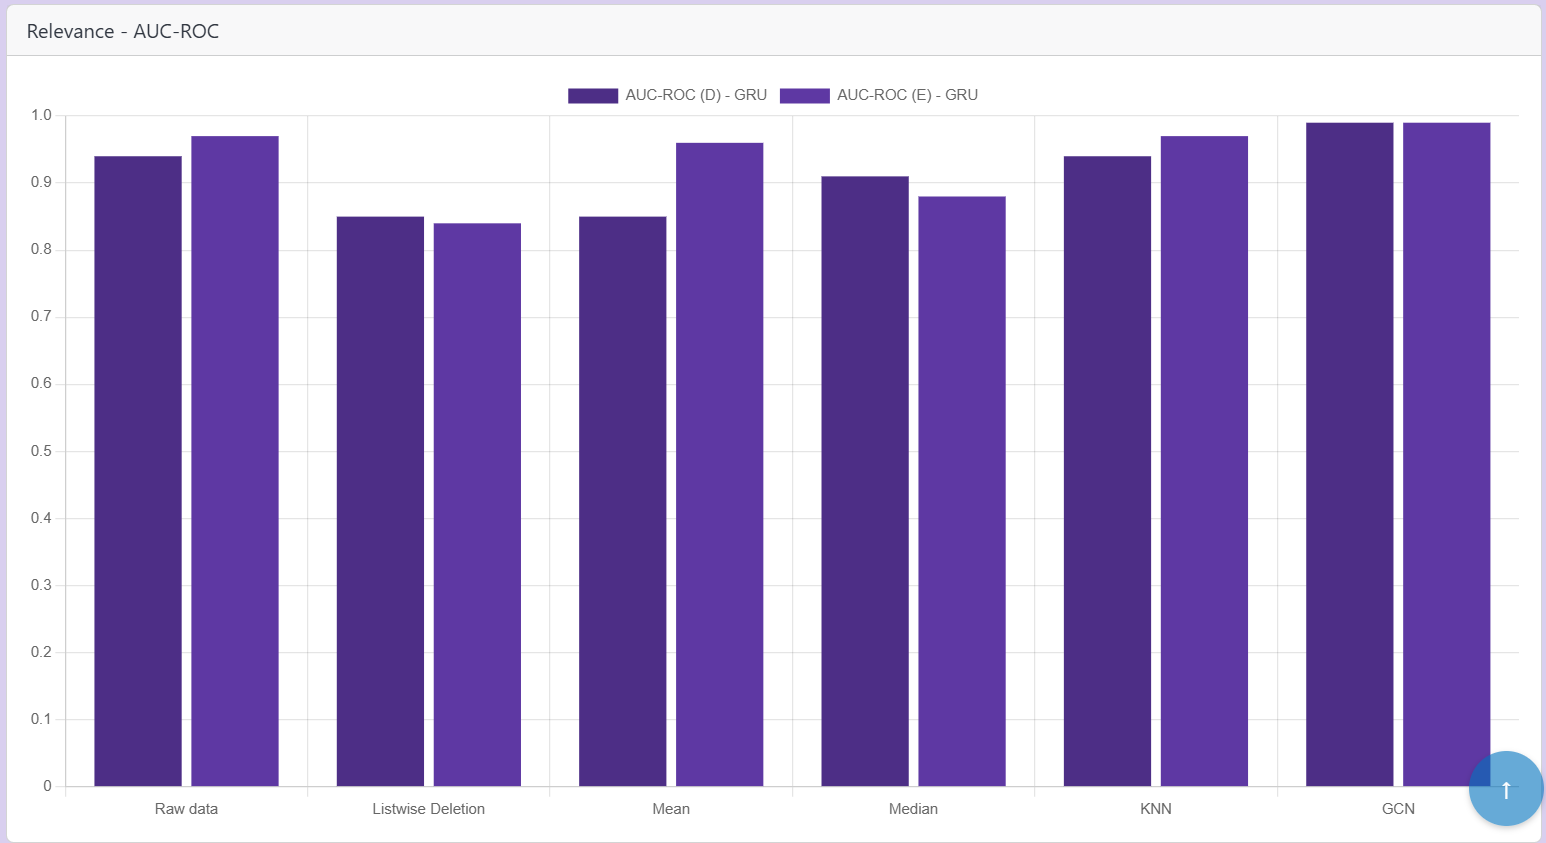
\includegraphics[width = 0.8\textwidth]{imgs/demo-15.png}
    \caption{AUC-ROC theo mô hình GRU}
    \label{fig:demo-15}
\end{figure}
\begin{figure}[H]
    \centering
    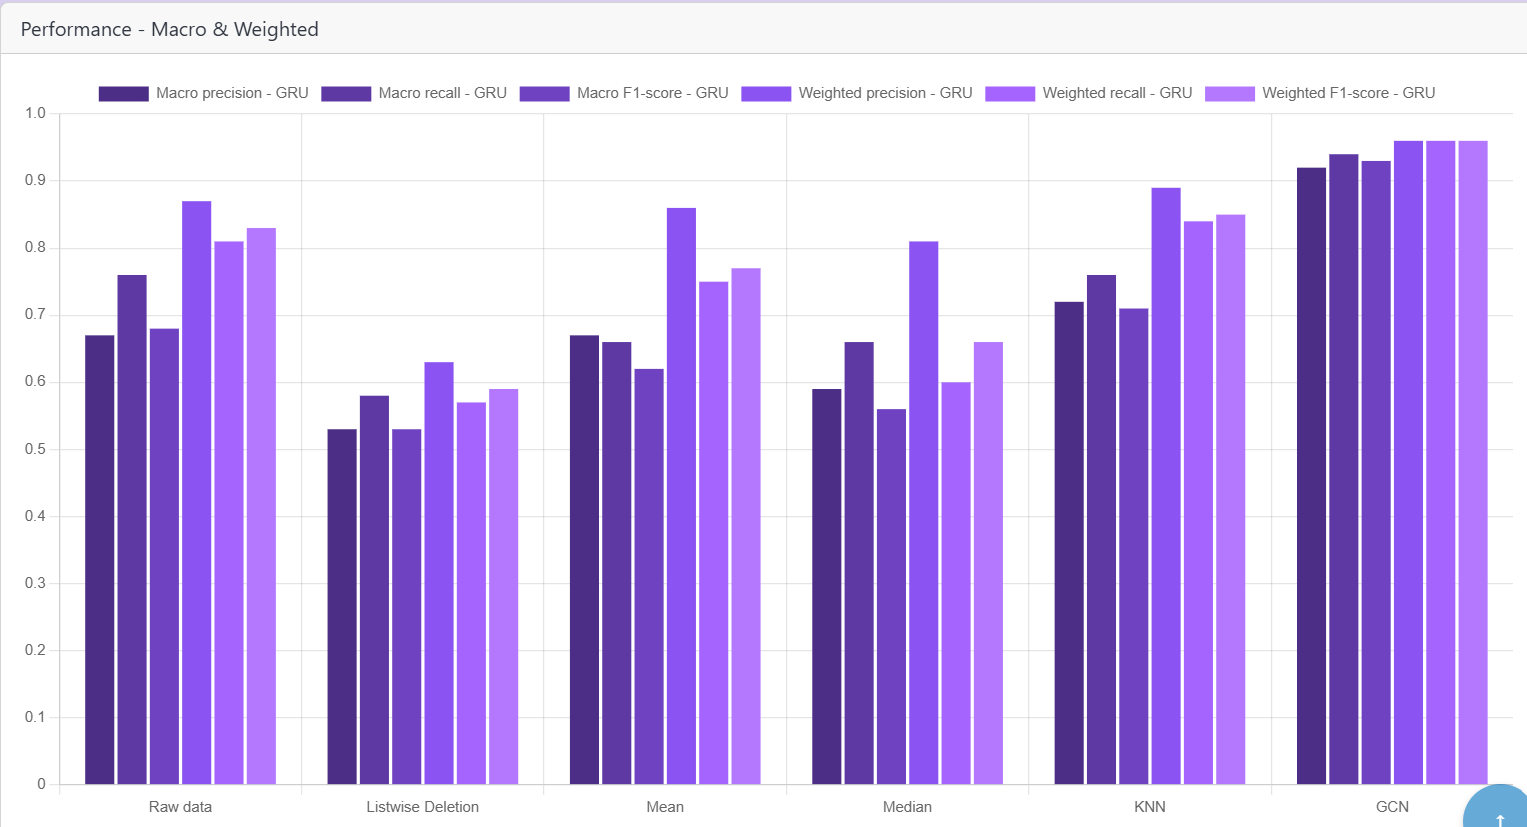
\includegraphics[width = 0.8\textwidth]{imgs/demo-16.png}
    \caption{Hiệu suất toàn diện mô hình GRU theo độ đo Macro và Weighted}
    \label{fig:demo-16}
\end{figure}

\chapter{Kết luận và hướng phát triển}
\label{chap:chap7}
% \section{Thảo luận}

% Trong bối cảnh dữ liệu học tập trực tuyến trên các nền tảng MOOCs thường rất phức tạp, đa dạng và không đồng nhất, việc xử lý và khai thác hiệu quả dữ liệu trở thành một thách thức lớn. Dữ liệu thường bao gồm nhiều loại thực thể khác nhau như người học, khóa học, các loại tương tác đa dạng (xem video, làm bài tập, thảo luận), đồng thời thường xuyên gặp tình trạng thiếu dữ liệu hoặc dữ liệu bị thưa thớt. Những vấn đề này ảnh hưởng nghiêm trọng đến chất lượng và độ chính xác của các mô hình dự đoán kết quả học tập.

% Phương pháp của chúng tôi tập trung vào sử dụng Graph Convolutional Networks (GCN) để điền khuyết (imputation) dữ liệu bị thiếu, tận dụng cấu trúc đồ thị tự nhiên của các mối quan hệ giữa người học và các đối tượng liên quan. GCN có khả năng khai thác hiệu quả thông tin từ cả đặc trưng bản thân từng node (thực thể) và các node láng giềng trong đồ thị, giúp mô hình nắm bắt được mối quan hệ phức tạp và ngữ cảnh của từng thực thể trong hệ thống. Điều này vượt trội hơn so với các phương pháp điền khuyết truyền thống chỉ dựa trên đặc trưng riêng lẻ của từng cá thể.

% Một trong những điểm mạnh nổi bật của GCN là khả năng khai thác thông tin gián tiếp thông qua các bước lan truyền trong đồ thị, nhờ đó làm tăng tính đầy đủ và chính xác của dữ liệu đầu vào sau khi điền khuyết. Việc này giúp giảm thiểu đáng kể vấn đề thiếu dữ liệu lịch sử (cold start) – vốn là một rào cản lớn trong các hệ thống dự đoán cá nhân hóa, đồng thời làm tăng tính ổn định và khả năng khái quát của các mô hình dự đoán.

% Sau khi dữ liệu được điền khuyết hoàn chỉnh, chúng tôi tiếp tục sử dụng các mô hình học sâu (deep learning) và thực hiện quá trình tinh chỉnh (fine-tuning) các mô hình này trên dữ liệu đầy đủ. Việc tinh chỉnh giúp mô hình học sâu khai thác sâu hơn các đặc trưng phức tạp, mối quan hệ phi tuyến tính giữa các biến số và các tương tác đa chiều trong dữ liệu học tập của người dùng. Nhờ đó, mô hình không chỉ có khả năng dự đoán chính xác hơn mà còn thích nghi tốt với các biến đổi hoặc dữ liệu mới, nâng cao hiệu quả trong thực tế ứng dụng.

% Việc kết hợp giữa điền khuyết dữ liệu bằng GCN và tinh chỉnh các mô hình học sâu tạo thành một chuỗi xử lý dữ liệu toàn diện, vừa giải quyết bài toán dữ liệu thiếu thưa, vừa nâng cao khả năng mô hình hóa các mối quan hệ phức tạp, từ đó cải thiện hiệu suất dự đoán kết quả hoàn thành khóa học một cách rõ rệt. Phương pháp này tận dụng tốt ưu điểm của cả hai kỹ thuật: GCN xử lý cấu trúc dữ liệu quan hệ, deep learning xử lý biểu diễn đặc trưng phi tuyến và phức tạp.

% Tuy nhiên, bên cạnh những ưu điểm vượt trội, phương pháp này cũng đặt ra một số thách thức. Việc sử dụng GCN và các mô hình deep learning yêu cầu tài nguyên tính toán lớn, đặc biệt khi làm việc với các bộ dữ liệu có quy mô lớn hoặc có nhiều tính chất phức tạp. Điều này có thể gây khó khăn trong việc triển khai thực tế, đòi hỏi các kỹ thuật tối ưu hóa và phần cứng phù hợp để đảm bảo khả năng mở rộng và tốc độ xử lý.

% Ngoài ra, chất lượng kết quả dự đoán vẫn phụ thuộc nhiều vào chất lượng dữ liệu gốc và hiệu quả của quá trình điền khuyết. Nếu dữ liệu ban đầu có nhiều lỗi hoặc thiếu quá nhiều thông tin, ngay cả GCN cũng có thể không hoàn toàn khắc phục được, dẫn đến giảm hiệu quả của các bước xử lý tiếp theo. Do đó, việc đảm bảo tính nhất quán, chính xác và làm sạch dữ liệu đầu vào vẫn là bước quan trọng không thể bỏ qua.

% Việc lựa chọn và tinh chỉnh các siêu tham số trong cả GCN và các mô hình học sâu cũng là yếu tố then chốt quyết định hiệu quả mô hình. Cần có chiến lược tìm kiếm tối ưu và đánh giá kỹ lưỡng để tránh hiện tượng quá khớp (overfitting) hoặc không đủ khả năng khái quát (underfitting), đồng thời cân bằng giữa độ chính xác dự đoán và chi phí tính toán.

% Tóm lại, phương pháp kết hợp điền khuyết bằng GCN và tinh chỉnh các mô hình deep learning được đánh giá là một giải pháp mạnh mẽ và hiệu quả trong việc dự đoán kết quả hoàn thành khóa học trên nền tảng MOOCs. Nó không chỉ nâng cao chất lượng dữ liệu đầu vào mà còn giúp mô hình học sâu tận dụng tối đa đặc trưng phức tạp, góp phần cải thiện độ chính xác và độ tin cậy của hệ thống dự đoán, mở ra nhiều hướng phát triển mới cho các nghiên cứu tiếp theo trong lĩnh vực phân tích và dự đoán dữ liệu học tập trực tuyến.

% % Dữ liệu thực tế vốn dĩ rất không đồng nhất, bao gồm nhiều loại thực thể khác nhau như người dùng, mặt hàng, danh mục và các tương tác. Các mạng thông tin dị hướng (HINs) có khả năng mô hình hóa hiệu quả các mối quan hệ này, cho phép tích hợp thông tin đa dạng. Các nhúng được tiền huấn luyện từ HINs có thể tổng quát hóa tốt hơn với dữ liệu chưa từng thấy nhờ việc tiếp xúc với một phổ rộng các mối quan hệ và ngữ cảnh trong quá trình huấn luyện. Điều này giúp giảm thiểu rủi ro bị quá khớp (overfitting) và nâng cao khả năng của mô hình trong việc thích ứng với các bộ dữ liệu mới và đa dạng.

% % Các nhúng từ HINs cung cấp một đại diện ban đầu toàn diện cho các tình huống khởi động lạnh (cold start), giúp giảm thiểu vấn đề thiếu dữ liệu lịch sử cho người dùng hoặc mặt hàng mới. Bằng cách tận dụng thông tin cấu trúc từ HINs, H-BERT4Rec trở nên ít nhạy cảm hơn với độ thưa thớt của dữ liệu, đảm bảo các khuyến nghị đáng tin cậy ngay cả khi các tương tác giữa người dùng và mặt hàng còn hạn chế. Tuy nhiên, việc xây dựng H-BERT4Rec cũng đối mặt với một số hạn chế và điểm cần cân nhắc:

% % \begin{enumerate}
% %     \item Kết hợp HINs với BERT có thể yêu cầu tài nguyên tính toán đáng kể, đặc biệt là đối với các bộ dữ liệu lớn, dẫn đến các vấn đề về khả năng mở rộng. Cần có các chiến lược hiệu quả cho việc xử lý và tối ưu hóa dữ liệu để giải quyết vấn đề này.
% %     \item Việc tạo ra và duy trì HINs đòi hỏi quản lý và tích hợp dữ liệu cẩn thận để đảm bảo độ chính xác và nhất quán. Các lỗi trong dữ liệu hoặc các mối quan hệ có thể dẫn đến các nhúng không tối ưu và làm suy giảm hiệu suất của hệ thống khuyến nghị.
% %     \item Tối ưu hóa các tham số có tác động đáng kể đến hiệu quả của mô hình (chẳng hạn như $N$, $d$, hoặc $\alpha, \beta, \theta$), và việc chấp nhận các đánh đổi trong các chỉ số ít hiệu quả hơn (ví dụ: một số thước đo có thể giảm, và tốc độ khuyến nghị có thể giảm khi N tăng lên).
% % \end{enumerate}

\section{Tổng kết}

Trong khuôn khổ của khóa luận, các nội dung nghiên cứu đã được trình bày một cách hệ thống và đa chiều, tập trung vào việc đề xuất và triển khai phương pháp điền khuyết dữ liệu học tập trong môi trường MOOC dựa trên mạng nơ-ron tích chập đồ thị. Phương pháp đề xuất GCN-I đã được đánh giá thông qua một loạt thí nghiệm thực tế, kết hợp với các mô hình học sâu phổ biến, cho thấy nhiều kết quả khả quan.

Các đóng góp chính của khóa luận bao gồm:
(1) Đề xuất phương pháp \textbf{GCN-I} tận dụng cấu trúc liên kết giữa người học và khóa học để điền khuyết dữ liệu, từ đó nâng cao chất lượng dữ liệu đầu vào và đạt kết quả vượt trội so với các kỹ thuật truyền thống như \textit{Mean}, \textit{Median}, \textit{Listwise Deletion}, hay KNN, với độ chính xác đạt \textbf{95\%}, F1-score cho lớp \textbf{D} đạt \textbf{0.92}, và chỉ số \textbf{AUC-ROC} lên đến \textbf{0.99};
(2) Thiết kế và triển khai hệ thống thực nghiệm gồm bốn mô hình học sâu phổ biến là \textbf{RNN}, \textbf{GRU}, \textbf{LSTM}, và \textbf{BiLSTM}, trong đó \textbf{GRU} đạt hiệu suất cao nhất;
(3) Phân tích chi tiết hiệu quả mô hình trên các lớp dữ liệu khan hiếm, đặc biệt là lớp \textbf{D}, vốn thường bị bỏ qua do mất cân bằng nghiêm trọng;
(4) Xây dựng hệ thống website \textbf{SmartEduTrack} có giao diện thân thiện, hỗ trợ người quản lý khóa học theo dõi quá trình học tập và dự đoán khả năng hoàn thành khóa học của từng người học, góp phần nâng cao hiệu quả giảng dạy trong môi trường trực tuyến.

Dựa trên những kết quả thu được có thể kết luận việc điền khuyết dữ liệu một cách có cấu trúc và thông minh bằng \textbf{GCN}, cùng với các mô hình học sâu, không chỉ khả thi mà còn có hiệu quả vượt trội trong bối cảnh dữ liệu thực tế. Đây là đóng góp quan trọng của khóa luận trong việc mở rộng ứng dụng học máy vào lĩnh vực giáo dục trực tuyến trong thời đại số.

\section{Hướng phát triển}

Khóa luận đã tập trung khai thác tiềm năng của mạng nơ-ron tích chập trên đồ thị (GCNs) để giải quyết bài toán dữ liệu thưa thớt trên nền tảng MOOCs, đồng thời kết hợp với  công nghệ học sâu nhằm dự đoán kết quả hoàn thành khóa học chính xác và ổn định và xây dựng thành công website SmartEduTrack. Những kết quả chúng tôi đạt được là cơ sở để đạt được nhiều thành tựu mới trong tương lai. Cụ thể:

\begin{enumerate}
    \item \textbf{Mở rộng biểu diễn đồ thị học tập:} Hiện tại, dữ liệu được mô hình chỉ là các kết nối cơ bản giữa người học với nhau và người học với khóa học. Việc tích hợp thêm các yếu tố như chủ đề bài học, phản hồi người học, hoạt động trong diễn đàn, hoặc hành vi truy cập nội dung để xây dựng đồ thị học tập toàn diện hơn giúp mô hình học được ngữ cảnh phong phú và chính xác hơn từ dữ liệu quan sát.

    \item \textbf{Ứng dụng các biến thể GCN nâng cao:} Áp dụng các kỹ thuật mới như GAT (Graph Attention Networks), GCN động hoặc GCN có yếu tố thời gian sẽ cho phép mô hình học tập hiệu quả hơn trong các tình huống dữ liệu thay đổi liên tục, đặc biệt với hành vi người học theo thời gian. Các biến thể này cũng có thể cải thiện khả năng khôi phục dữ liệu thực tế.

    \item \textbf{Sử dụng các mô hình học máy hiện đại:} Các mô hình học sâu mạnh hơn như Transformer hoặc BERT, nhằm tận dụng dữ liệu đã được cải thiện qua GCN có thể được tích hợp. Việc điều chỉnh và tối ưu các mô hình giúp kết quả dự đoán được cải thiện không chỉ về độ chính xác mà còn khoảng thời gian dự đoán.

    \item \textbf{Hướng tới dự đoán thời gian thực:} Việc xây dựng hệ thống dự đoán có khả năng cập nhật và phản hồi theo thời gian thực sẽ là bước tiến quan trọng, giúp giảng viên và quản lý khóa học can thiệp kịp thời. Điều này đòi hỏi kết hợp mô hình với các kiến trúc tính toán hiệu quả như học trực tuyến (online learning) hoặc xử lý phân tán.

    \item \textbf{Phát triển thêm các chức năng ứng dụng:} Từ phương pháp được đề xuất, có thể phát triển các dashboard tương tác cung cấp thông tin dự báo, gợi ý học tập cá nhân hóa và cảnh báo rủi ro không hoàn thành khóa học. Hệ thống này có thể tích hợp trực tiếp vào nền tảng MOOC để hỗ trợ giảng viên ra quyết định và đồng hành cùng người học trong suốt quá trình học tập.

    \item \textbf{Khả năng mở rộng và ứng dụng đa lĩnh vực:} Phương pháp GCN-I hoàn toàn có thể mở rộng áp dụng cho các nền tảng học trực tuyến khác như edX, Coursera, Udemy, cũng như các lĩnh vực có đặc điểm dữ liệu hành vi người dùng. Việc mở rộng này không chỉ cho phép kiểm tra khả năng tổng quát hóa của phương pháp mà còn tạo ra giá trị ứng dụng thực tiễn rộng rãi.
\end{enumerate}

Các kết quả đạt được trong khóa luận này chỉ là bước khởi đầu cho một chặng đường nghiên cứu dài hơn. Việc tiếp tục phát triển các định hướng đã gợi mở sẽ đóng vai trò then chốt trong việc gia tăng giá trị khoa học và tác động thực tiễn của đề tài. Cụ thể, các nỗ lực trong tương lai sẽ không chỉ tập trung vào việc tối ưu hóa các phương pháp đã xây dựng, mà còn mở rộng khả năng ứng dụng của chúng trong nhiều bối cảnh đa dạng. Quá trình này sẽ đồng thời củng cố nền tảng lý thuyết và là tiền đề để phát triển các giải pháp đổi mới, đáp ứng hiệu quả hơn các thách thức trong giáo dục trực tuyến. Hơn nữa, việc theo đuổi các định hướng này sẽ là cầu nối cho các nghiên cứu liên ngành, qua đó nâng cao giá trị khoa học ứng dụng thực tế.


% Appendix chapter in thesis
%include{chapters/back/MAPR2024_LongHoangNguyen/apendixA}

% Print references
\printbibliography[heading=bibintoc, title = {Tài liệu tham khảo}]

\appendix
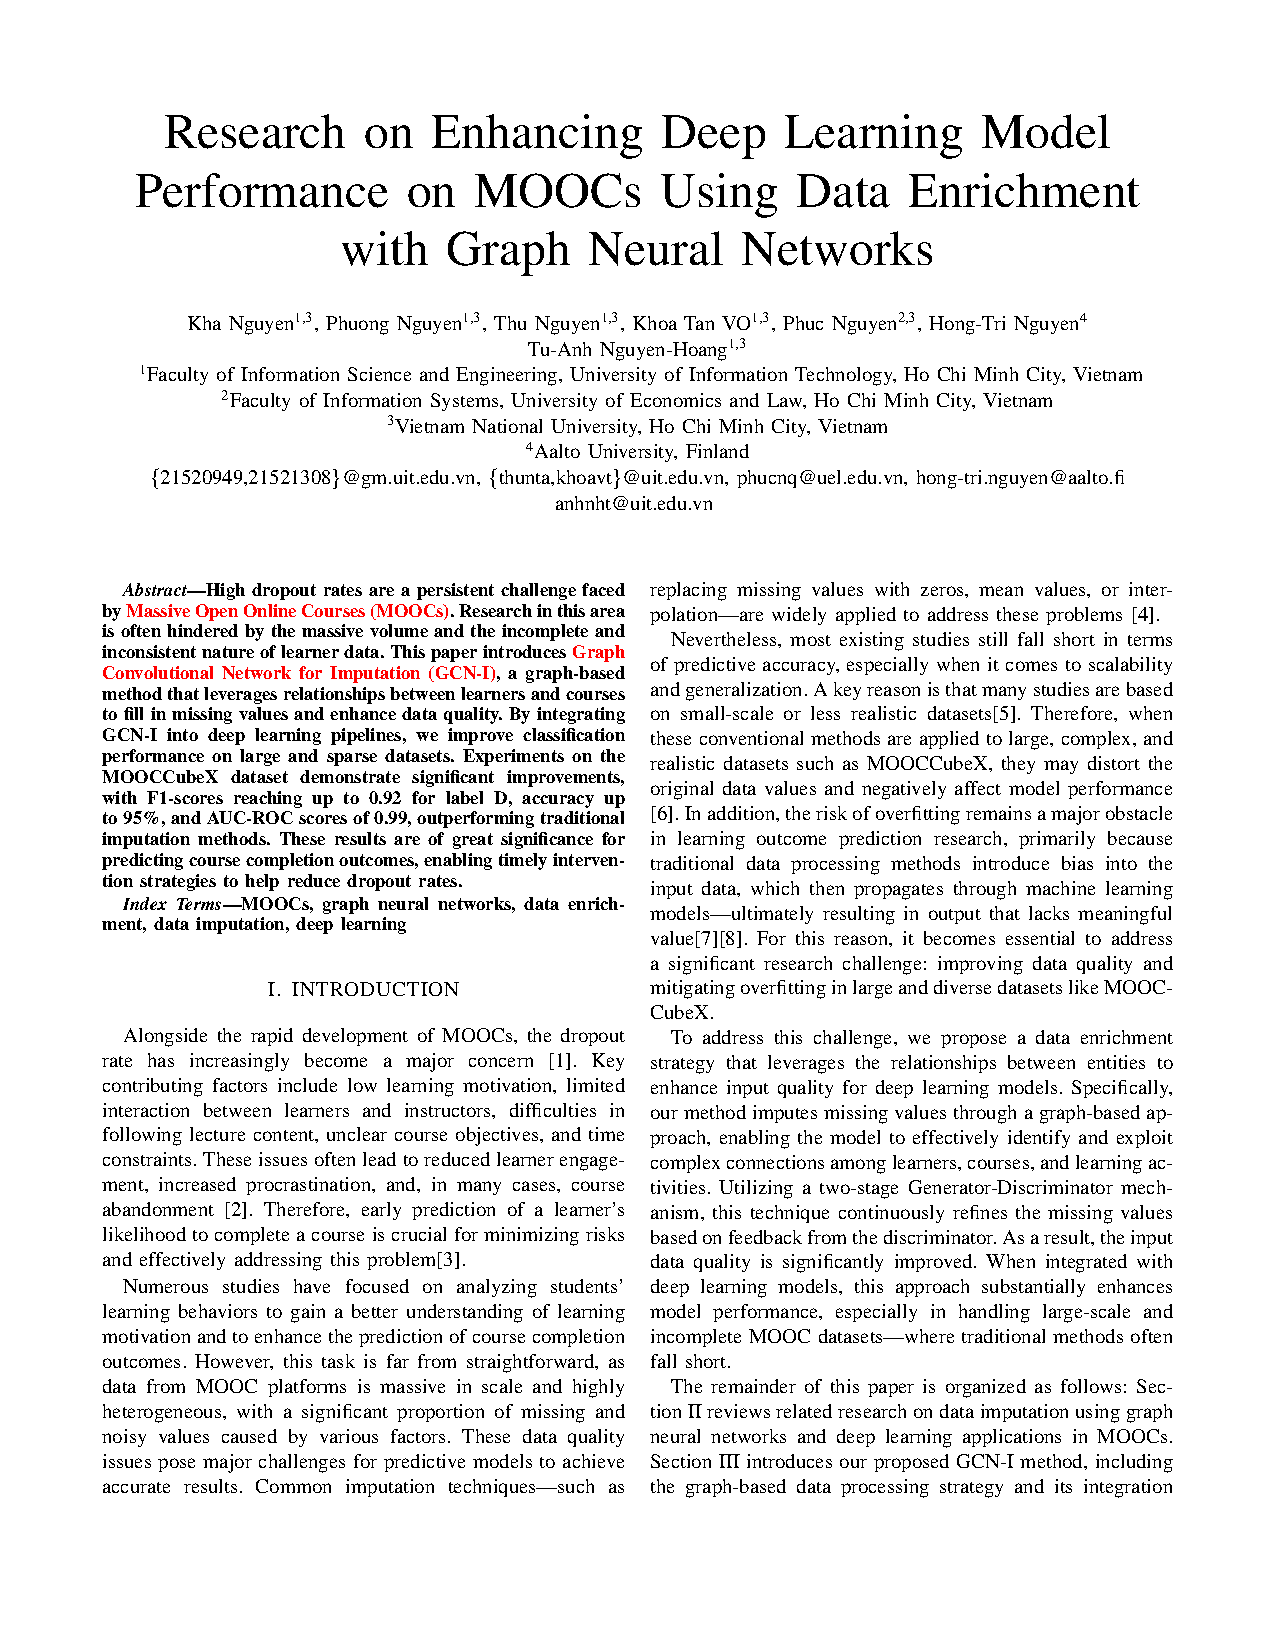
\includepdf[page={1-7}]{ICCAE2026.pdf}
\end{document}
